\chapter{Introduction}
\section{Motivation}
The heat present in the earth's crust has been recognized as a potential energy source for the generation of electricity for nearly a century, and has been exploited to this end for nearly 60 years in multiple locations \citep{Gregg_1958,GARRISON_1972,Minissale_1991}. To date, the worldwide installed geothermal capacity is over 14 GWe spread across more than 50 countries \citep{Pan_2019, Bertani_2016}, with the potential for substantially more through the creation of enhanced geothermal systems (EGS) \citep{Blackwell_2007}. Due to the confluence of abundant, naturally-fractured reservoirs, high heat flow and relatively low startup cost, New Zealand was one of the first countries to adopt geothermal as a source of electricity and currently has the fifth largest installed geothermal capacity in the world, accounting for roughly 16 percent of the nation's electricity generation \citep{Bertani_2016,Grant_2011}. However, the future growth of geothermal technologies is uncertain due to a number of associated risks including high startup costs \citep{Olasolo_2016} and the potential impact of induced seismicity (IS) related to injection and withdrawal of fluids \citep{Majer_2007,Ellsworth_2013}.

In the last decade, interest in IS has grown in the scientific and industrial communities as well as in the public sphere \citep{Ellsworth_2013}. Mostly, this is a result of the remarkable increase in seismicity in places such as Oklahoma, Arkansas, Texas and Ohio where wastewater related to hydrocarbon production is being injected into the subsurface \citep[e.g.][]{Yeck_2017,Horton_2012,Kim_2013,McGarr_2017,Keranen_2013}. In addition, a number of geothermal projects have been abandoned or postponed due to the occurrence of larger-than-expected seismic events \citep[e.g.][]{Deichmann_2009,Grigoli_2018}. Given the incomplete understanding of the processes which generate such seismicity, it is difficult to reliably forecast its extent, magnitude and timing for a given injection or extraction scenario. However, these processes are thought to include: injection pressure, flow rate, temperature and total volume, reservoir temperature, permeability and size, subsurface structure, injection proximity to basement formations, and the subsurface stress state. As public and regulatory scrutiny of IS increases, it will become increasingly important to understand the detailed interactions between each of these factors in order to design strategies to mitigate the risk of generating large, damaging earthquakes \citep[e.g.][]{Langenbruch_2017}.

When viewed from a different perspective, the occurrence of human-induced seismicity presents a unique setting in which earthquakes can be observed at locations and times which are fully or partially known a priori. The ability to generate seismicity through controlled, measurable actions  offers us the opportunity to study, in great detail, the processes which lead to seismogenesis \citep[e.g.][]{Raleigh_1976}. These results can then be applied more widely to problems of natural (and often more damaging) seismicity.

Lest we forget that injection operations serve a purpose other than generating earthquakes, datasets of IS contain useful information regarding reservoir properties such as flow pathways, permeability structure and fracture geometry. From an operational standpoint, this information is critical in managing a dynamic resource like a geothermal reservoir \citep{Majer_2007}. This final point is the key to the work presented in this thesis.

In this work, we focus on the Ngatamariki and Rotokawa geothermal fields in the Taup\={o} Volcanic Zone (TVZ) of central New Zealand, from mid-2012 until the end of 2015. Both fields are exclusively operated by Mercury NZ Ltd. The catalog of seismicity we have created is an indicator of processes occurring within the reservoirs that are otherwise difficult to measure without drilling additional wells (and spending much more money). These catalogs offer clues to the orientation and size of the fracture network, geometry of flow pathways, reservoir transmissivity, and stress state in the reservoir. This insight is especially useful where reservoir behavior cannot be fully explained by well-based measurements.

\section{Study Aims}
The primary goal of this thesis is to establish quantifiable relationships between the occurrence of seismicity and power production operations, specifically fluid extraction and injection, at the Rotokawa and Ngatamariki geothermal fields. The specific research questions that we will address are as follows:

\begin{enumerate}
  \item{How do variations in the rate, location and magnitude of seismicity at each field relate to the injection and withdrawal of fluid?}
  \item{Can a relationship be established between well stimulation (i.e. permeability increase) and seismicity?}
  \item{Do earthquake focal mechanisms aid in characterizing the orientation and extent of the reservoir fracture network?}
  \item{What can spatial and temporal variations in stress state tell us about injection and production-related changes to the reservoir?}
\end{enumerate}

In order to answer these questions, we constructed a comprehensive catalog of seismicity for both fields. This process included the completion of the following tasks:
\begin{itemize}
  \item{Compile an automatically-detected catalog of seismicity (Question 1, Chapter 2);}
  \item{Detect additional, smaller-magnitude events using events compiled above as templates using a matched-filter routine \citep{Chamberlain_2017} (Question 1--2, Chapters 2--4);}
  \item{Relocate entire catalog using a non-linear, grid search algorithm \citep{Lomax_2014}, with locations further refined by a relative-relocation algorithm \citep{Trugman_2017} (Question 1--2, Chapters 2--5);}
  \item{Write and implement a magnitude estimation methodology \citep{Shelly_2016} for events detected using the matched-filter technique (Question 1-2, Chapters 2--4);}
  \item{Manually pick P-wave first arrival polarities and invert for focal mechanism solutions \cite{Walsh_2009} (Question 3--4, Chapter 5);}
\end{itemize}

The analysis of this catalog as it relates to the injection and production operations at the fields involved the following additional step:
\begin{itemize}
  \item{Invert focal mechanism solutions for stress state over time and space \citep{Arnold_2007,Lund_2007} (Question 4, Chapter 5);}
\end{itemize}

The research presented here is funded by Mercury NZ Ltd., who have identified several periods of interest in which the reservoir behaved in unexpected or interesting ways. We will focus on addressing each of these periods in turn and relate the characteristics of seismicity within the reservoir to the parameters measured at the wells in question. The periods of interest are the following:\selectlanguage{english}

\begin{table}
\begin{tabular}{cccc}
    {Field} & {Operation} & {Start} & {End}\\ \midrule
    Ngatamariki & NM08 Stimulation & June-2012 & July-2012\\
    Ngatamariki & NM09 Stimulation & December-2012 & January-2013\\
    Ngatamariki & NM10 Drilling Losses & July-2012 & August-2012\\
    Ngatamariki & NM12 Drilling Losses  & June-2014 & September-2014\\
    Rotokawa & RK24 Injectivity Decline & 2012 & 2013\\
    Rotokawa & Switch of Injection: RK24-RK23 & June-2014 & July-2014\\
    Rotokawa & RK34 Drilling Losses & September-2014 & November-2014\\
    Rotokawa & Plant Shutdowns and Startups & 2012-2015 & 2012-2015\\
\end{tabular}
\caption{{Table summarizing the key periods of interest specified by Mercury for the years 2012-2015. These periods define the focus of study for comparing
changes in well parameters to the response in seismicity.}}
\label{table:objectives}
\end{table}

\section{Geothermal Power}
\subsection{Power Production}
Geothermal electricity generation relies on converting the heat energy from the earth to mechanical energy, which is used to turn a generator. Heat is extracted from the subsurface through extraction of a gas or liquid phase that is heated by conduction from the reservoir rock. Therefore, a commercially viable geothermal reservoir requires high temperature at accessible depths (via rotary drilling) and sufficient permeability, which enables rapid transport of fluid to the surface. As a general rule, the temperature of the earth's crust increases with depth at an average of 30\textdegree{C}\slash{km} \citep{Grant_2011}. On a more localized level, however, gradients of 100\textdegree C or greater can be encountered \citep{Grant_2011}. All modern, produced geothermal fields are convective systems, meaning that the pressure and temperature distribution in the field is governed not by conductive heat transfer, but by the circulation of hot fluids through permeable rock \citep{Grant_2011}. These types of fields can be broken into two basic types: liquid-dominated and vapor-dominated (of which there are few), based on the dominant fluid phase present in the reservoir. Both Ngatamariki and Rotokawa are liquid-dominated reservoirs \citep{McNamara_2016,Chambefort_2016}.

There are a variety of field configurations, but most modern geothermal fields consist of a production field, where fluid is drawn out of the reservoir, and an injection field where some portion (up to nearly 100 percent) of the extracted fluid is reinjected back into the reservoir. This is done for a number of reasons, the most important of which is to maintaining reservoir pressure and volume to avoid degrading the resource \citep{Grant_2011}. The injection and production field are connected via the power plant (or multiple plants) that uses the extracted fluid either directly or indirectly (i.e. a binary plant) to turn a turbine and generate electricity. There are many variations on the heat-to-electricity conversion system, and the choice of which to use at a particular field is governed by the dominant fluid phase in the reservoir and the reservoir temperature \citep{DiPippo_2016}. For the purposes of this thesis, we are concerned with binary (Figure \ref{836935}B), flash-steam (Figure \ref{836935}A) and combined cycle (Figure \ref{836935}C) power plants, which are the types of plants installed at Ngatamariki and Rotokawa. A binary plant uses the fluid extracted from the reservoir to boil a highly-volatile, secondary fluid (for example, isopentane) with a much lower boiling point than the reservoir fluid, which is then used to turn a turbine. A flash steam plant, on the other hand, flashes the extracted reservoir fluid to steam, which is directly deployed in the turbine \citep{DiPippo_2016}. Combined cycle plants use both technologies simultaneously.

Two power plants are installed at Rotokawa. The first, a 24 MWe (megawatts electrical) combined-cycle plant, was installed in 1997, while the second, a 140 MWe, triple-flash plant named Nga Awa Purua (NAP), was installed in 2010 \citep{McNamara_2016}. Ngatamariki is the most recently-developed field in New Zealand, with the 82 MWe binary power plant coming online in 2013.\selectlanguage{english}

\begin{sidewaysfigure}[p]
\begin{center}
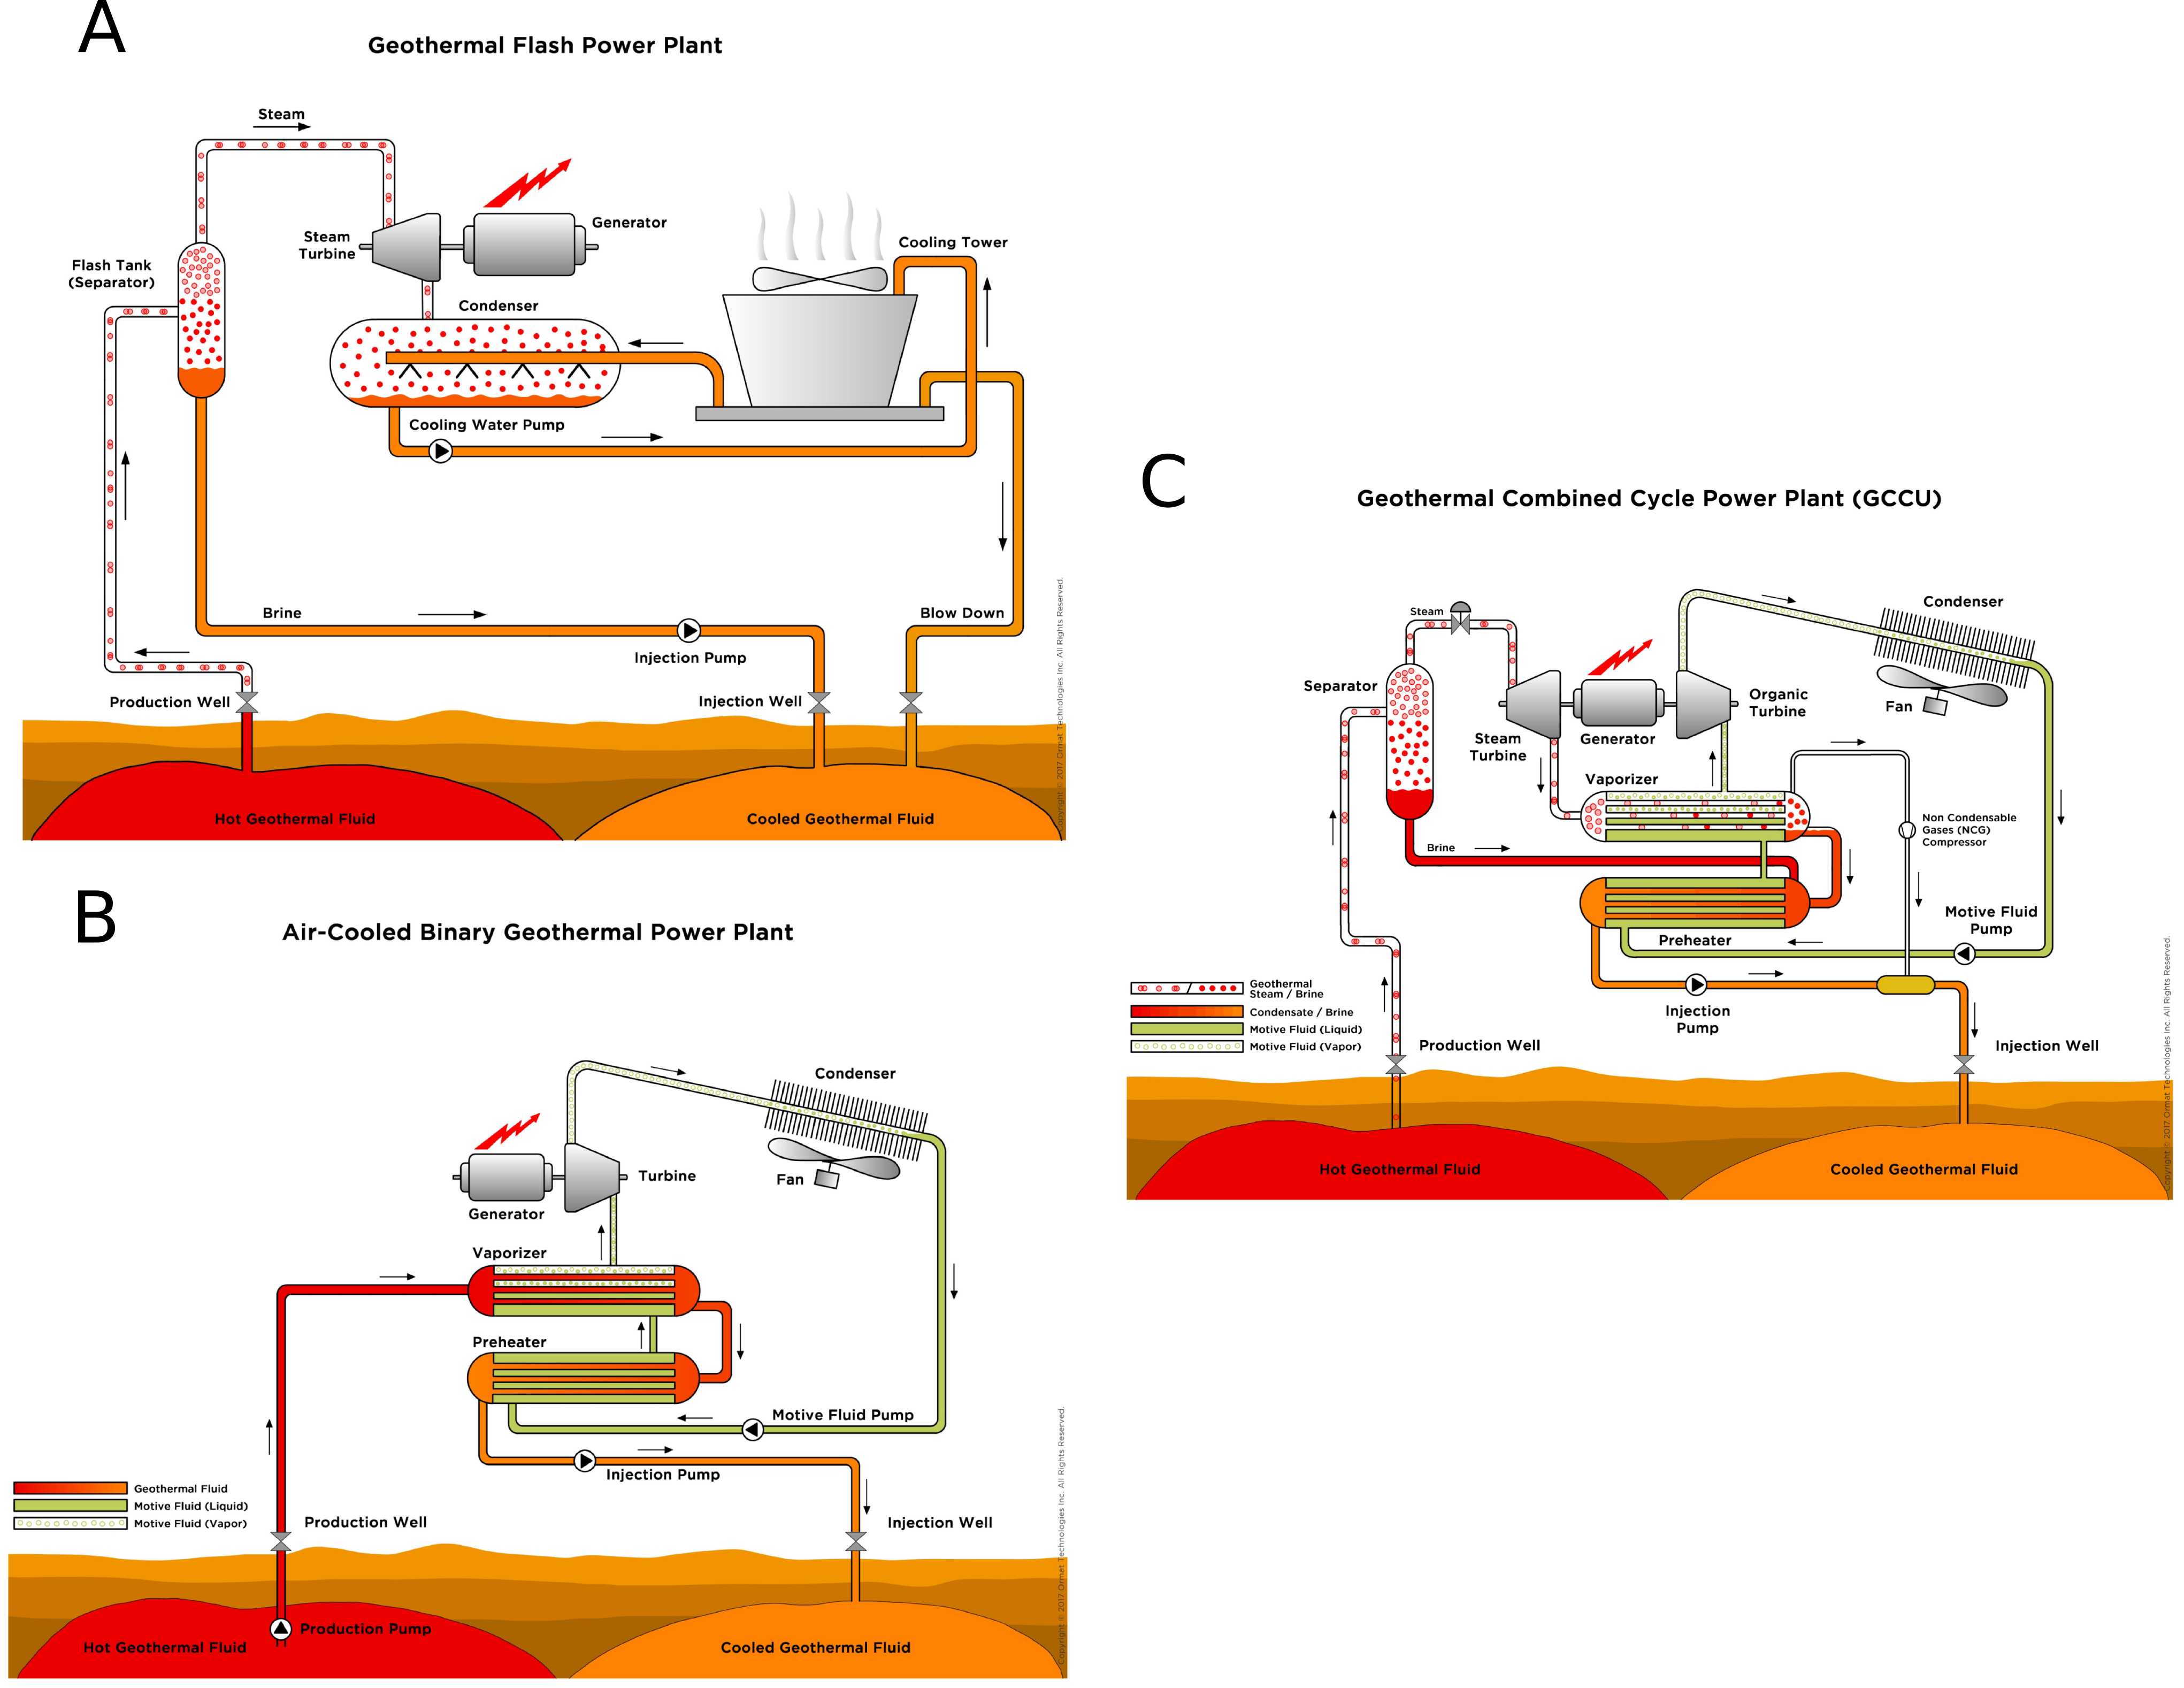
\includegraphics[width=\textwidth,height=0.5\textheight,keepaspectratio]{Chapter_1_Intro/figures/ORMAT_techs_overview/ORMAT_techs_overview_original.png}
\caption{{Schematics of the operation of three types of geothermal power plants:
A) Flash-steam, B) Binary and C) Combined cycle. At Rotokawa, the
original `RGEN' plant is type C, while the more recently-installed Nga
Awa Purua plant is a `triple-flash' variant of type A, meaning that
there are three separate stages of liquid-steam separation, which
increases plant efficiency~\protect\cite{DiPippo_2016}. The Ngatamariki plant is
type B. These figures are adapted from the Ormat 2017 Annual
Report~\protect\cite{Ormat_2018}
{\label{836935}}%
}}
\end{center}
\end{sidewaysfigure}

\section{Reservoir Management}
\subsection{Datasets}
Reservoir engineers, modelers, geologists and geophysicists use a number of data streams to assess the state of a given geothermal reservoir. Most of these data are derived from measurements taken inside the wells drilled into the resource, and provide a wealth of important information including \citep{DiPippo_2016,Grant_2011}:
\begin{itemize}
  \item{Geologic core}
  \item{Natural-state temperatures}
  \item{Pressure-temperature spinner (PTS) data}
  \item{Image logs (Fracture orientation/aperture/spacing and borehole breakout)}
  \item{Resistivity, porosity, density logs}
  \item{Injection and production flow rate}
  \item{Injection and production pressures}
  \item{Injection temperature and chemistry}
  \item{Radioactive tracer tests}
\end{itemize}
These datasets allow operators to constrain the spatial extent, temperature distribution and permeability in the reservoir. However, these data are sparsely sampled relative to the total reservoir area due to the prohibitive cost of drilling deep wells. To aid in interpreting the data listed above, other geophyisical and geochemical data are often collected at the surface, which include:
\begin{itemize}
  \item{Magnetotelluric surveys}
  \item{Microgravity surveys}
  \item{Leveling (subsidence monitoring)}
  \item{Spring/fumarole temperature and chemistry}
  \item{Active-source seismic}
\end{itemize}

Seismic data occupy a unique place in the spectrum of data available to geothermal operators. While waveform data are collected at the surface (or in some cases at 100s of meters depth in boreholes), they are the surface manifestation of fracture rupture (i.e. strain) at depth in the reservoir, a process which is affected by the distribution of reservoir temperature and pressure. Pressure and temperature can be accurately measured at wells, but seismicity can occur throughout a reservoir and therefore gives a much more densely-sampled view of fluid movement within the reservoir. For the purposes of this thesis, we will focus on the characterization of reservoir seismicity and its relation to many of the well parameters listed above. The most important constraints on state of the reservoir come from well pressure and flow rate data, both of which will feature prominently in the work that follows. 

\subsection{Terms and Definitions}\label{terms}

When assessing the relationship between seismicity and reservoir management, we generally focus on injection, as opposed to production. This is mostly because the withdrawl of fluids decreases pore-fluid pressure and, therefore, usually stabilizes reservoir fracture networks \citep{Segall_1994,Segall_1998}(see further discussion in Section \ref{mechanisms}). However, not all injection operations are the same, and each has a specific set of goals that will be important to understand in the context of IS at Rotokawa and Ngatamariki:
\begin{itemize}
  \item{\textbf{Brine reinjection}}
  
  During the normal operation of a power plant, brine is extracted from the reservoir, put through the power plant, and reinjected. This type of operation makes up the bulk of the reinjection operations in our dataset. This type of reinjection, in the case of the two fields considered here, is characterized by high flow rates (up to $\sim$1000 t/h), high temperatures ($\sim$90\textdegree C) and an injectate chemistry consistent with that of the reservoir fluid. Reinjection at Rotokawa during our 2012-2015 study period is entirely of this type as there was little new well development.
  \item{\textbf{Completion Testing}}
  
  Once a well has been drilled, engineers and modelers need to be able to estimate the extent and permeability of the reservoir in order to better estimate its future behavior. To do this, completion tests are conducted by varying the flow rate into (or out of) the well, and measuring the resulting pressure response \citep{horne1995modern}. At Ngatamariki, completion testing was done with river water ($\sim$15\textdegree C) at moderate flow rates of up to 200 t/h. No new wells were drilled at Rotokawa during our study period, and therefore no completion tests were conducted.
  \item{\textbf{Stimulation Testing}}
  
  Stimulation testing refers to the injection of fluid with the express purpose of measuring the change in the permeability of the well. This is important, as the flow rates during injection testing are usually much lower than those required to run the power plant to its full capacity. In the case of a binary plant (type B, Figure \ref{836935}) where the geothermal fluid circulates through the system in a closed loop, the operator needs to be able to reinject nearly 100 percent of this extracted volume. Therefore, an estimation of the potential of a well to accept increasing volumes of fluid is essential in accurately modeling the feasibility of the entire power scheme once the plant comes online \citep{DiPippo_2016,Grant_2011}.
  
  In high-temperature geothermal reservoirs, stimulation is likely associated with thermal contraction of the walls of the fractures though which fluid is flowing \citep{grant2013thermal}, which may manifest as aseismic opening of the fractures \citep[e.g.][]{Guglielmi_2015}. However, stimulation may also be related to seismic slip on fractures through which permeability can be either increased or decreased, an effect which has been extensively studied in the lab and through numerical simulations \citep[e.g.][and references therein]{Lee_2002,Fang_2017}. See Section \ref{mechanisms} for further discussion of stimulation and permeability changes.
\end{itemize}

With these injection scenarios in mind, it will be useful to define at the outset of this thesis certain basic terms and quantities that we will lean on in the following chapters:
\begin{itemize}
  \item{\acrfull{WHP}}
  \item{\acrfull{DHP}}
  \item{\Gls{flow_rate}}
  \item{\acrfull{II}}
  \item{\Gls{stimulation}}
  \item{\Gls{permeability}}
  \item{\Gls{transmissivity}}
  \item{\Gls{diffusivity}}
\end{itemize}

Measuring reservoir pressure is of paramount importance to assessing the state of the resource. This quantity can be measured in the well at or near the depth of the reservoir, in which case the measurement is referred to as \gls{DHP_g} (\acrshort{DHP}). If the pressure measurement is taken at the wellhead (\gls{WHP_g}, \acrshort{WHP}), however, some basic corrections need to be made to estimate the reservoir pressure at depth. Assuming a static water column in the well:

\begin{equation}
WHP = P_{r} - \rho{g}Z
\end{equation}

where $P_{r}$ is the reservoir pressure and $\rho{g}Z$ is the weight of the water column at depth $Z$. However, if the well is flowing, as is generally the case for wells in a geothermal field \citep{grant2013thermal,Clearwater_2015}:

\begin{equation}
WHP = P_{r} - \rho{g}Z + \frac{W}{II} + KW^{2}
\end{equation}

Where $W$ is mass \gls{flow_rate} (typically measured in tonnes per hour in New Zealand) and $KW^{2}$ is a term accounting for the frictional forces related to fluid flow down the well. \acrshort{II} is the \gls{II_g}, typically referred to simply as `injectivity', which is a measure of the well's ability to accept fluid at a given pressure. The \acrshort{II} relationship is calculated as \citep{DiPippo_2016}:

\begin{equation}
II = \frac{W}{P_{w} - P_{r}}
\end{equation}

where $P_{w} - P_{r}$ is the difference in pressure between the well and reservoir (overpressure). The increase in \acrshort{II} is typically referred to as `\gls{stimulation}', which can be thought of as an increase of the permeability of a well. Geothermal operators typically `stimulate' both production and injection wells once they have been drilled in order to increase the amount of fluid that can be drawn out of, or put into, the reservoir prior to plant startup.

\citet{grant2013thermal} suggest that geothermal wells stimulate as a power of time according to the empirical relationship: $II = Ct^{n}$ where $C$ is a constant, $t$ is time since the start of injection and $n$ has a value between 0.3 and 0.7 for the wells considered in the study \citep{grant2013thermal}. Figure \ref{415417} shows this relationship during the stimulation of NM08 at Ngatamariki \citep{Clearwater_2015}, which stimulated according to $n\approx0.7$.\selectlanguage{english}

\begin{figure}[h!]
\begin{center}
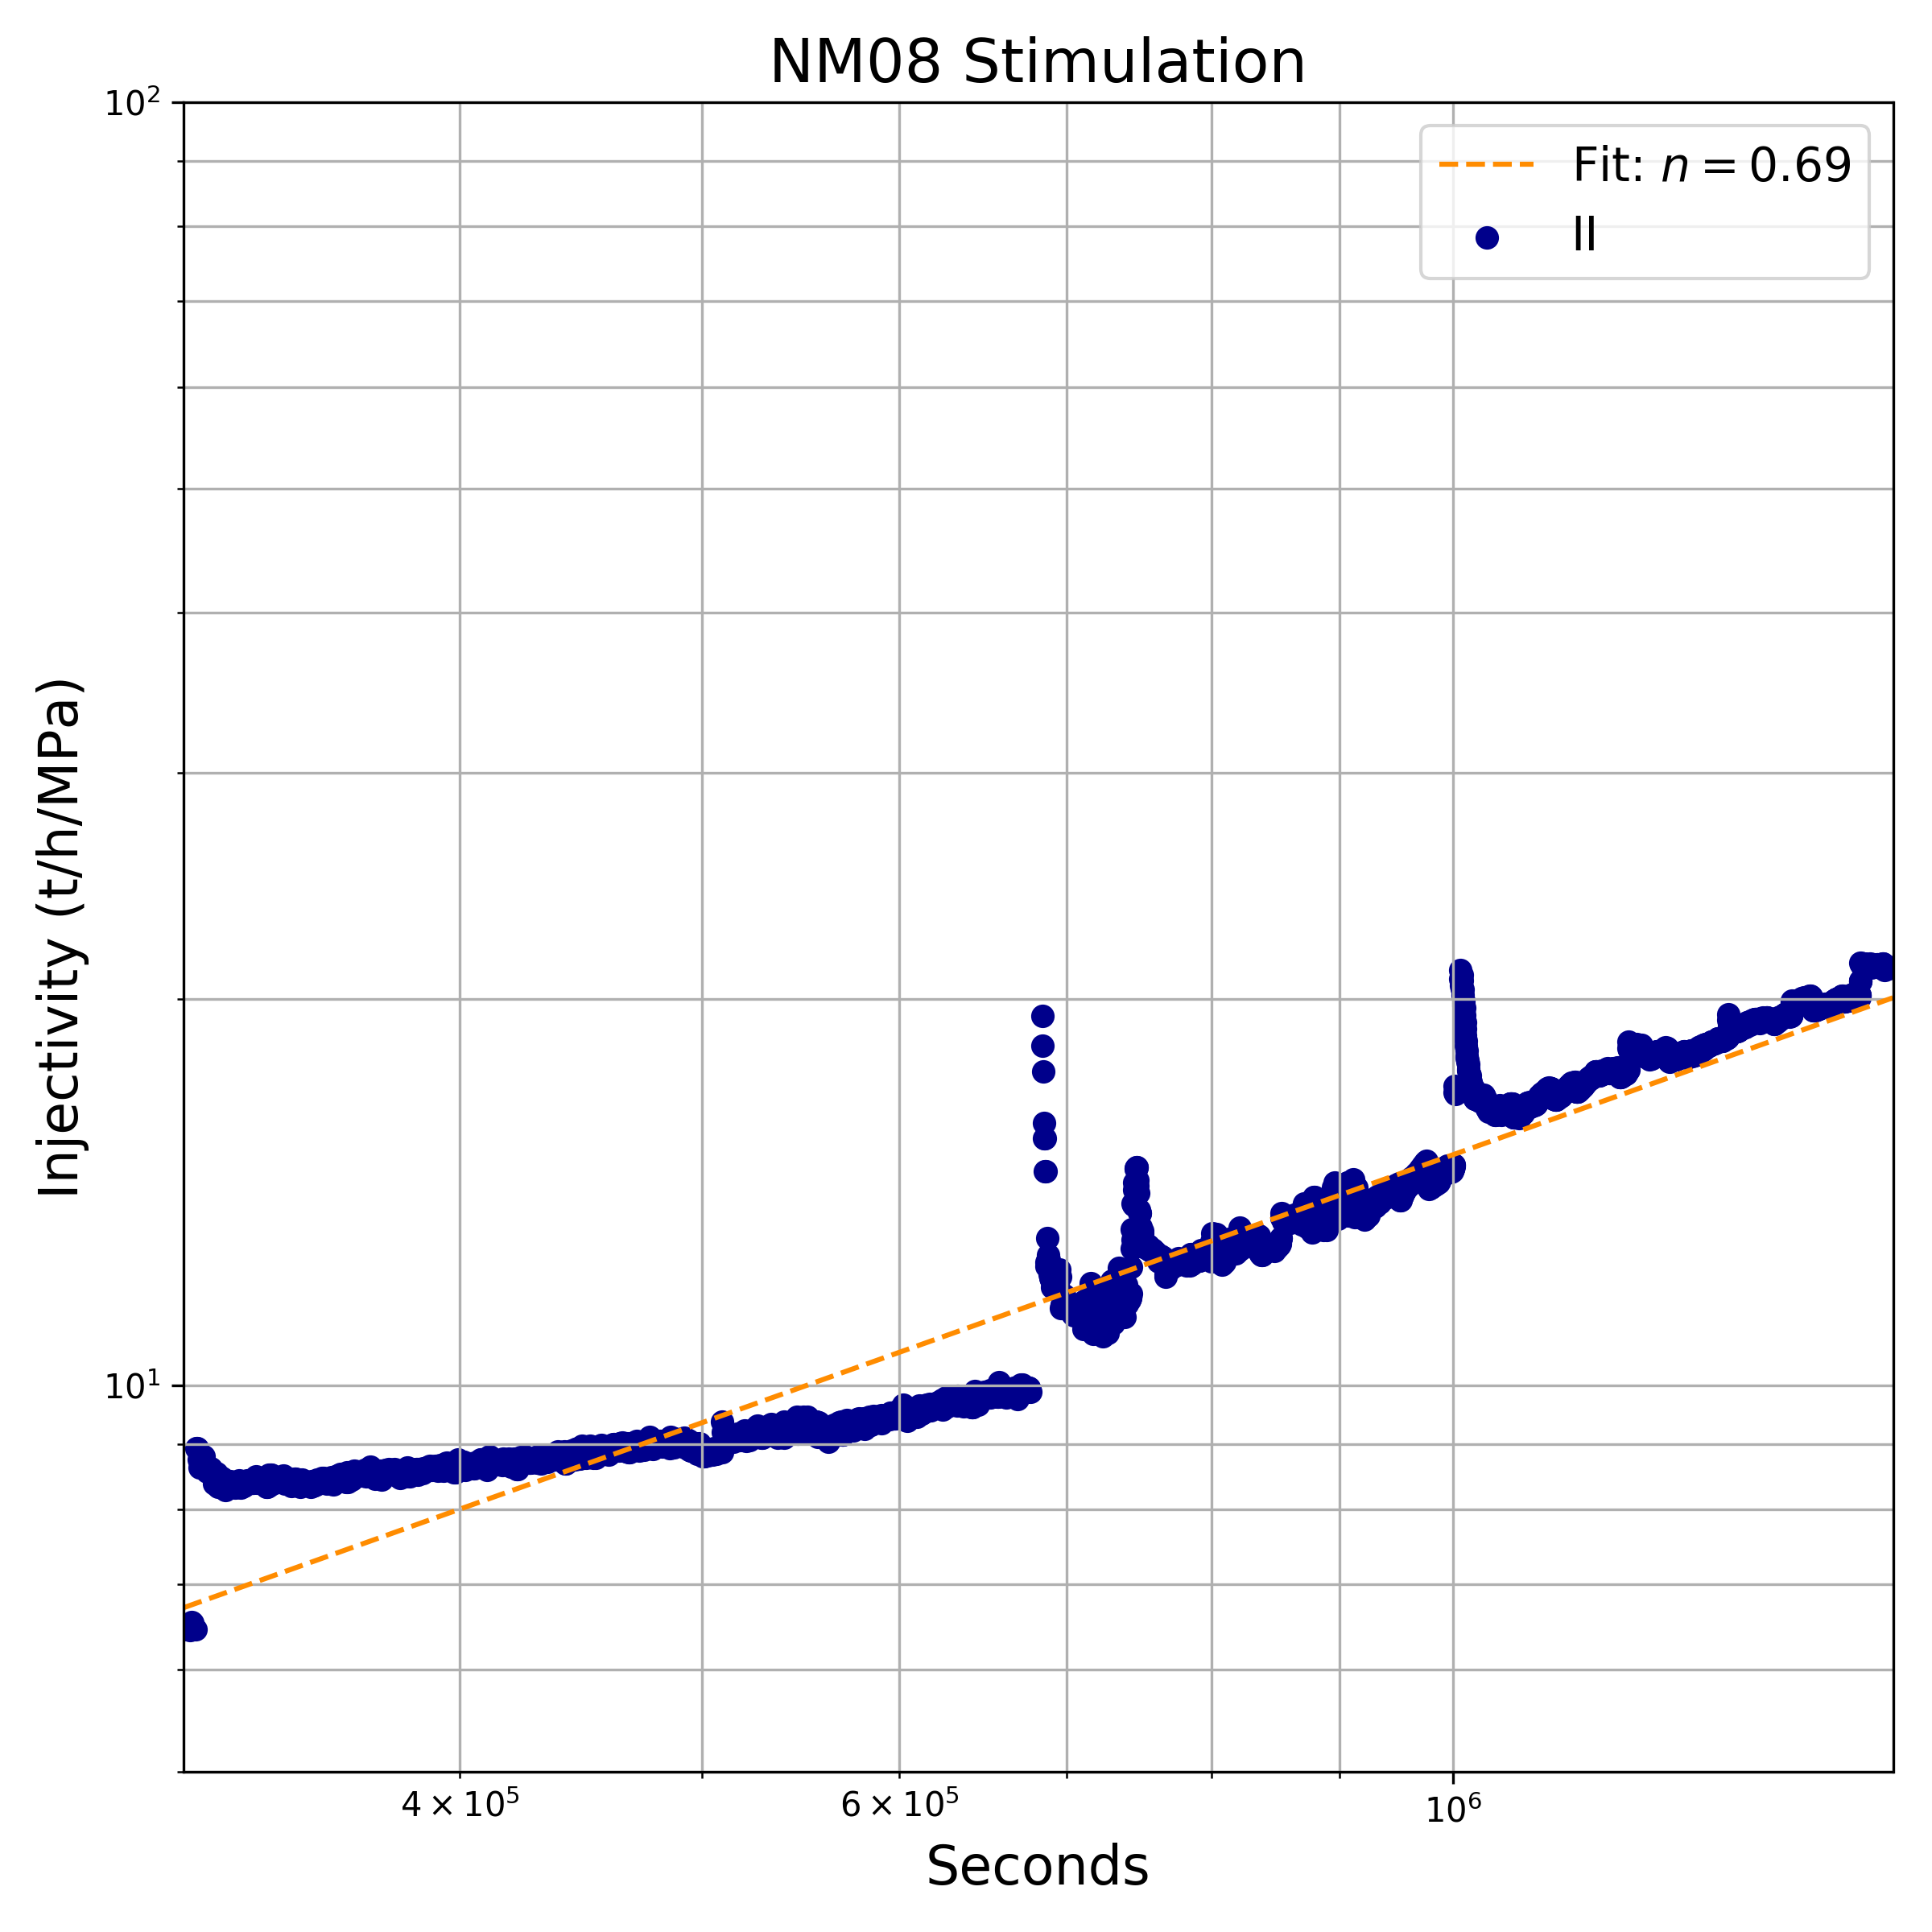
\includegraphics[width=0.70\columnwidth]{Chapter_1_Intro/figures/NM08_JC_ported_II_fitted/NM08_JC_ported_II_fitted_original}
\caption{{Injectivity of NM08 during a portion of the June 2012
stimulation\slash{completion} test. The rate of stimulation agrees with an
\(n\approx0.7\) relationship, which is higher than what is typically
observed at geothermal wells.
{\label{415417}}%
}}
\end{center}
\end{figure}

\Gls{permeability} is perhaps the most important property of a geothermal reservoir. It describes the ease with which fluid flows through a medium, and is the primary control on how much fluid can be taken out of, and put back into the reservoir, ultimately determining how much power can be generated \citep{Grant_2011}. As defined by Darcy's Law, \gls{permeability} is \citep{DiPippo_2016}:

\begin{equation}
k = \nu\frac{\mu{h}}{\Delta{P}}
\end{equation}

where $k$ is the reservoir permeability (m$^2$), $\nu$ is the fluid flow velocity through the reservoir (m/s), $\mu$ is the dynamic viscosity of the fluid (Pa$\cdot$s), $h$ is the thickness of the reservoir (m) and $\Delta{P}$ is the applied pressure difference (Pa).

\Gls{transmissivity} is the permeability-thickness product:

\begin{equation}
T = kh
\end{equation}

It describes the capacity of fluid to flow through a reservoir of thickness, $h$, but is often more convenient to work with than permeability. This is because $kh$ is easily estimated during standard well testing operations, and because the dimensions of the reservoir (i.e. $h$) are generally unknown.

Hydraulic \gls{diffusivity} is related to the permeability by:

\begin{equation}
D = \frac{k}{\mu{s}}
\end{equation}

where $D$ is \gls{diffusivity}, $\mu$ is fluid viscosity and $s$ is the storativity of the reservoir. The diffusion of a pore fluid pressure perturbation from a well has been shown to correspond to the volume within which induced seismicity is likely to occur \citep[e.g.][]{Shapiro_2002,Parotidis_2004,Shapiro_2009,Shapiro_1997,Jeanne_2014}. This use of earthquake hypocenters to infer reservoir properties is known as seismicity-based reservoir characteriztion (SBRC) \citep{Shapiro_2002} and will be detailed in Section \ref{IS}.

\section{Geology, Development and Conceptual Models}
\subsection{Taup\={o} Volcanic Zone}
With the exception of one (Ngawha), every producing geothermal field in New Zealand is located in the central North Island. This concentration of high heat flow is known as the Taup\={o} Volcanic Zone (TVZ) \ref{764580}, an area of backarc extension and volcanism at the margin of the active Hikurangi Subduction Zone where the Pacific Plate subducts obliquely westward beneath the Australian Plate at a rate of $\sim$45 mm/yr \citep{Cole_1981,Wilson_1995,DeMets_1994}. In the overriding plate, the rate of extension occurring along the axis of the TVZ ranges from 15 mm/yr at the Bay of Plenty to \textless 5 mm/yr in the south \cite{Wallace_2004}, most of which is accommodated within the Taup\={o} Fault Belt (TFB) \cite{Villamor_2011}. Although there is currently some debate as to the extent of the TVZ and how it developed \citep[e.g.][]{Stern_2011,Wilson_1995}, here we will adopt the interpretation of \citet{Wilson_2016} where the TVZ is is divided into three temporal zones: the old, young and modern as well as three geographic zones: the northern, central and southern \citep{Wilson_1995,Wilson_2016}.

The evolution of the TVZ began with the advent of volcanic activity at roughly 2 Ma that continues to the present day. The old TVZ encompasses all identified vents and eruptive centers active during the period from the advent of volcanic activity until the emplacement of the Whakamaru Group ignimbrites (0.35 Ma), associated with the creation of the Whakamaru caldera (WH: white lines, Figure \ref{764580}) \citep{Wilson_1995}. The young TVZ then includes all vents active during the period from 0.35 Ma until the Rotoiti eruption of the Okataina caldera (65ka; Figure \ref{764580}), and the modern TVZ encompasses the most recent 65 ky of volcanism, with a broadly similar geometry to that of the young TVZ \citep{Wilson_1995,Wilson_2016}. With the exception of the Mangakino geothermal system, the boundary of the young TVZ encompasses all of the active geothermal systems in the TVZ (black dotted line; Figure \ref{764580}).

The three geographic zones of the TVZ are delineated based on eruption rates, manifestation and composition. The central TVZ (CTVZ) is characterized by heat flows of 700 mW/m$^2$ \citep{Bibby_1995} and \textgreater6000 km$^2$ of caldera-forming, rhyolitic volcanism \citep{Wilson_1995} (calderas, Figure \ref{764580}). The northern and southern zones (northeast of Kawerau and southwest of Tokaanu, outside the bounds of Figure \ref{764580}) are characterized by andesite-dacite composite cones (larger in the south) and very little rhyolitic or basaltic products. The eruptive rates in the south are less than one third and heat flow one fifth of those in the central TVZ \citep{Wilson_2016}. These values are poorly constrained in the north, mostly due to its subaqueous nature, but the output is likely even less than that in the south \citep{Wilson_2016}.

The CTVZ, where all of the active geothermal systems are located, is made up of at least eight separate, rhyolite calderas, of which the two most recently active are Taup\={o} in the southwest and Okataina in the northeast \citep{Wilson_1995}. The Ngatamariki and Rotokawa systems both lie at the eastern edge of the 0.35 Ma Whakamaru caldera and within the Taup\={o}-Reporoa Basin (TRB) \citep{Wilson_2016,Downs_2014} (Figure \ref{764580}). Heat flow within the TRB is the highest in the TVZ, as evidenced by the concentration of geothermal systems \citep{Wilson_2016}. However, the TRB is sparsely faulted relative to the Taup\={o} Fault Belt to the west, where most of the active extension is accommodated (indicated by the high concentration of faults in Figure \ref{764580}). The reasons for this discrepancy are poorly understood and the interactions between modern tectonics, inherited structures (i.e. caldera rims and basement faults), magmatism and heatflow will need to be unraveled before sense can be made of the locations of CTVZ geothermal systems.\selectlanguage{english}

\begin{figure}[h!]
\begin{center}
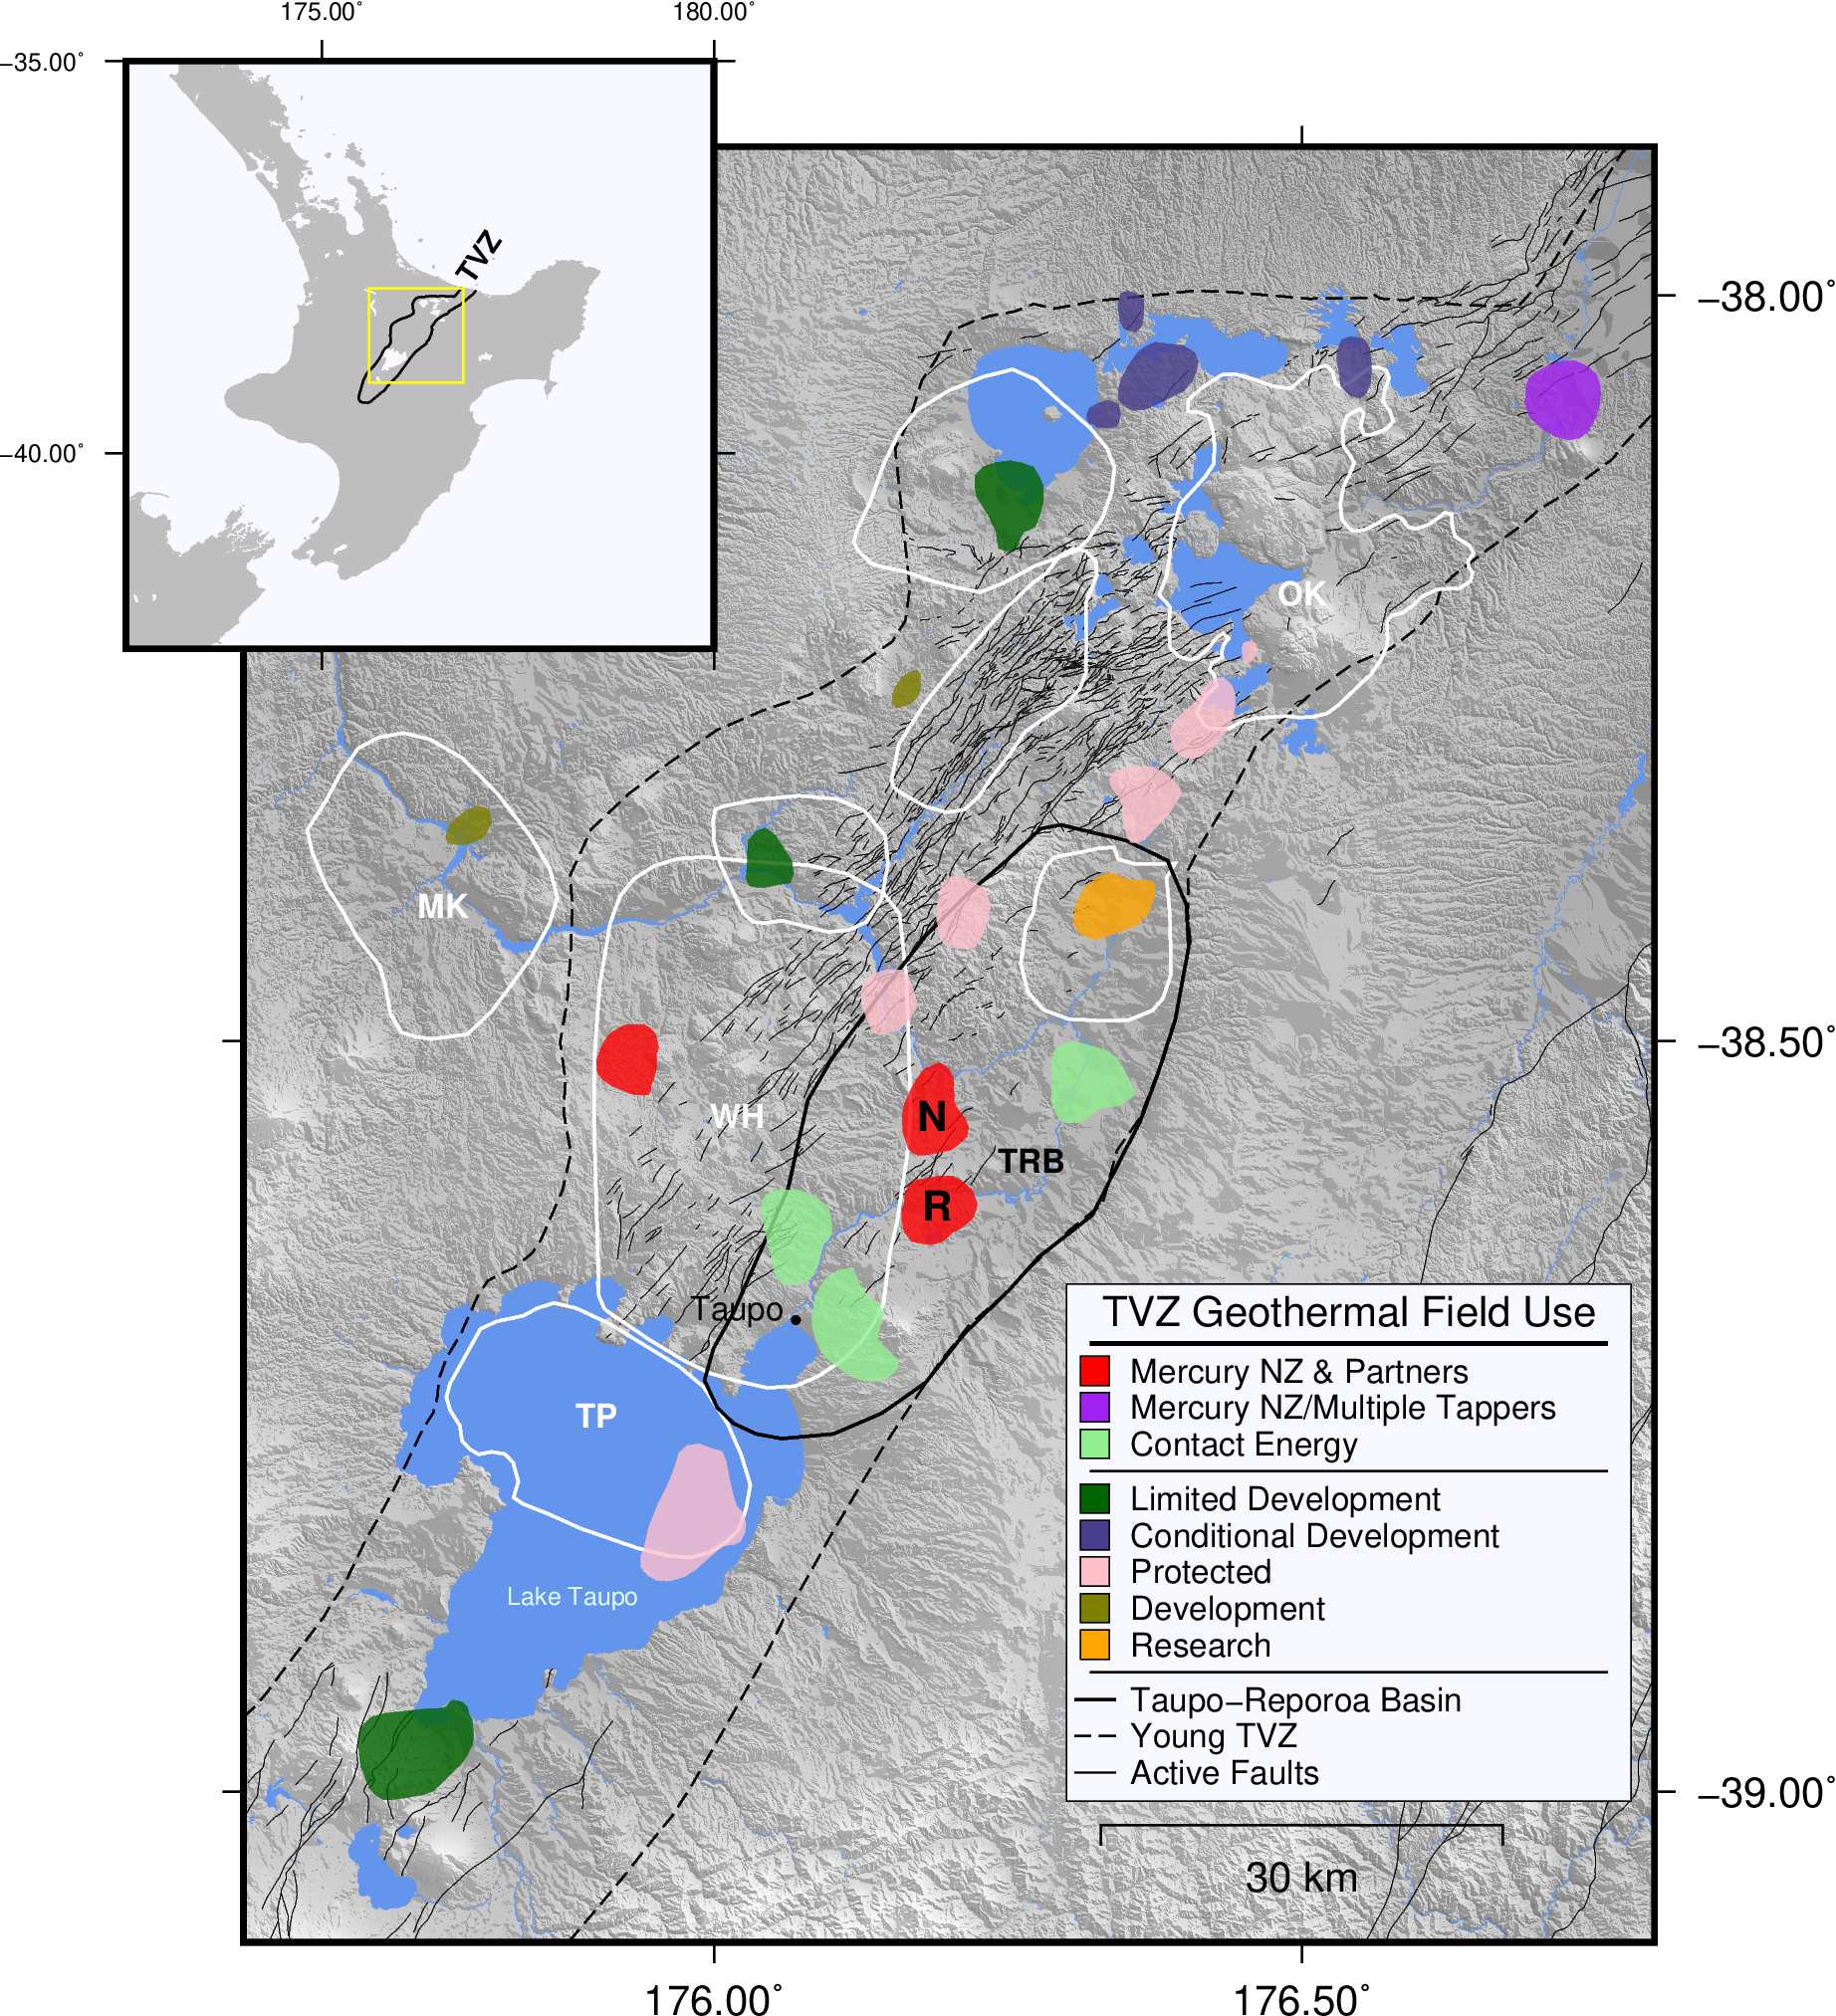
\includegraphics[width=1.00\columnwidth]{Chapter_1_Intro/figures/Geothermal_fields_TVZ_w_usage/TVZ_geothermal_overview_large}
\caption{{The resistivity boundaries of the 23 geothermal fields in the Central
Taup\={o} Volcanic Zone (CTVZ) (after \protect\citet{Bibby_1995}) colored by degree
of development or geothermal operator. Rotokawa and Ngatamariki are
labeled `R' and `N', respectively. The boundary of the young TVZ, as
defined by~\protect\citet{Wilson_1995} ,~ is shown as a dotted line and their
eight identified rhyolitic calderas are outlined in white (Whakamaru
Caldera: `WH', Taup\={o} Caldera: `TP', Okataina: 'OK', Mangakino: 'MK'). The Taup\={o}-Reporoa
Basin (TRB) is outlined in thick black after~\protect\citet{Downs_2014}.~~
{\label{764580}}%
}}
\end{center}
\end{figure}

\subsection{Ngatamariki}
\subsubsection{Geology}
The Ngatamariki geothermal field is located approximately 17 km north of the town of Taup\={o} (Figure \ref{425195}). Ngatamariki is a high-temperature, liquid-dominated and naturally-fractured system (up to 280\textdegree{}C at depths exceeding 1000 m) that measures roughly 5.5 km from north to south and 3 km east to west \citep{Bignall_2009, Chambefort_2014}. The reservoir is hosted in volcanic rocks of pre-Whakamaru age, known as the Reporoa Group (old TVZ, \textgreater0.35 Ma)\citep{Chambefort_2014}. In the southern portion of the field, the earliest unit in the Repora Group is the Rotokawa Andesite, which overlies the Torlesse Greywacke basement and, therefore, represents the onset of volcanism in the TVZ \citep{Chambefort_2014,Wilson_2016} (Figure \ref{673646}). The overlying units are referred to as the Tahorakuri Formation and consist of older andesitic lava flows and younger volcaniclastic units of varying composition, accounting for $\sim$1 Ma of volcanism \citep{Chambefort_2014}. In the northern part of the field, the upper Tahorakuri volcanic sequence is overlain by a sedimentary succession that is interpreted to represent a period of relative volcanic quiescence and active tectonism \citep{Chambefort_2014}. At that time, the Ngatamariki intrusive complex was emplaced in the northern part of the field, the only such plutonic body yet sampled in the TVZ \citep{Chambefort_2014}. This $\sim$0.7 Ma tonalite-diorite body defines the deeper portion (\textgreater2000 m bsl) of the northern reservoir, where in the south the Rotokawa Andesite is found \citep{Chambefort_2014} (Figure \ref{673646}). Overlying the Tahorakuri across most of the field is the Whakamaru Group ignimbrite, associated with the creation of the Whakamaru Caldera (WH, Figure \ref{764580}) and start of young TVZ volcanism \citep{Chambefort_2014,Wilson_1995}. The younger overlying units represent various periods volcanism and sedimentation through to the deposition of the modern surface deposits \citep{Chambefort_2014} (Figure \ref{673646}).

There are a number of mapped (Figure \ref{425195}) and buried (Figure \ref{673646}) normal faults within the Ngatamariki reservoir, defining small horst and grabben structures at depth \citep{Bignall_2009}. In the south, the larger of these structures are related to the active NE-SW Aratiatia Fault Zone (Figure \ref{425195}), while in the northern reservoir faulting is less extensive at the surface \citep{AFDB}. The primary structural trend in the field is NE-SW, related to the current extensional tectonic regime, with a subordinate NNW-SSE trend that has been attributed to the fabric of the Whakamaru caldera margin \citep{Bignall_2009}. This trend extends from the scale of mapped faults down to centimeter-scale fractures as interpreted from well image logs in both the northern and southern parts of the field \citep{nm09_report,nm10_report,massiot_2012}.\selectlanguage{english}

\begin{figure}[h!]
\begin{center}
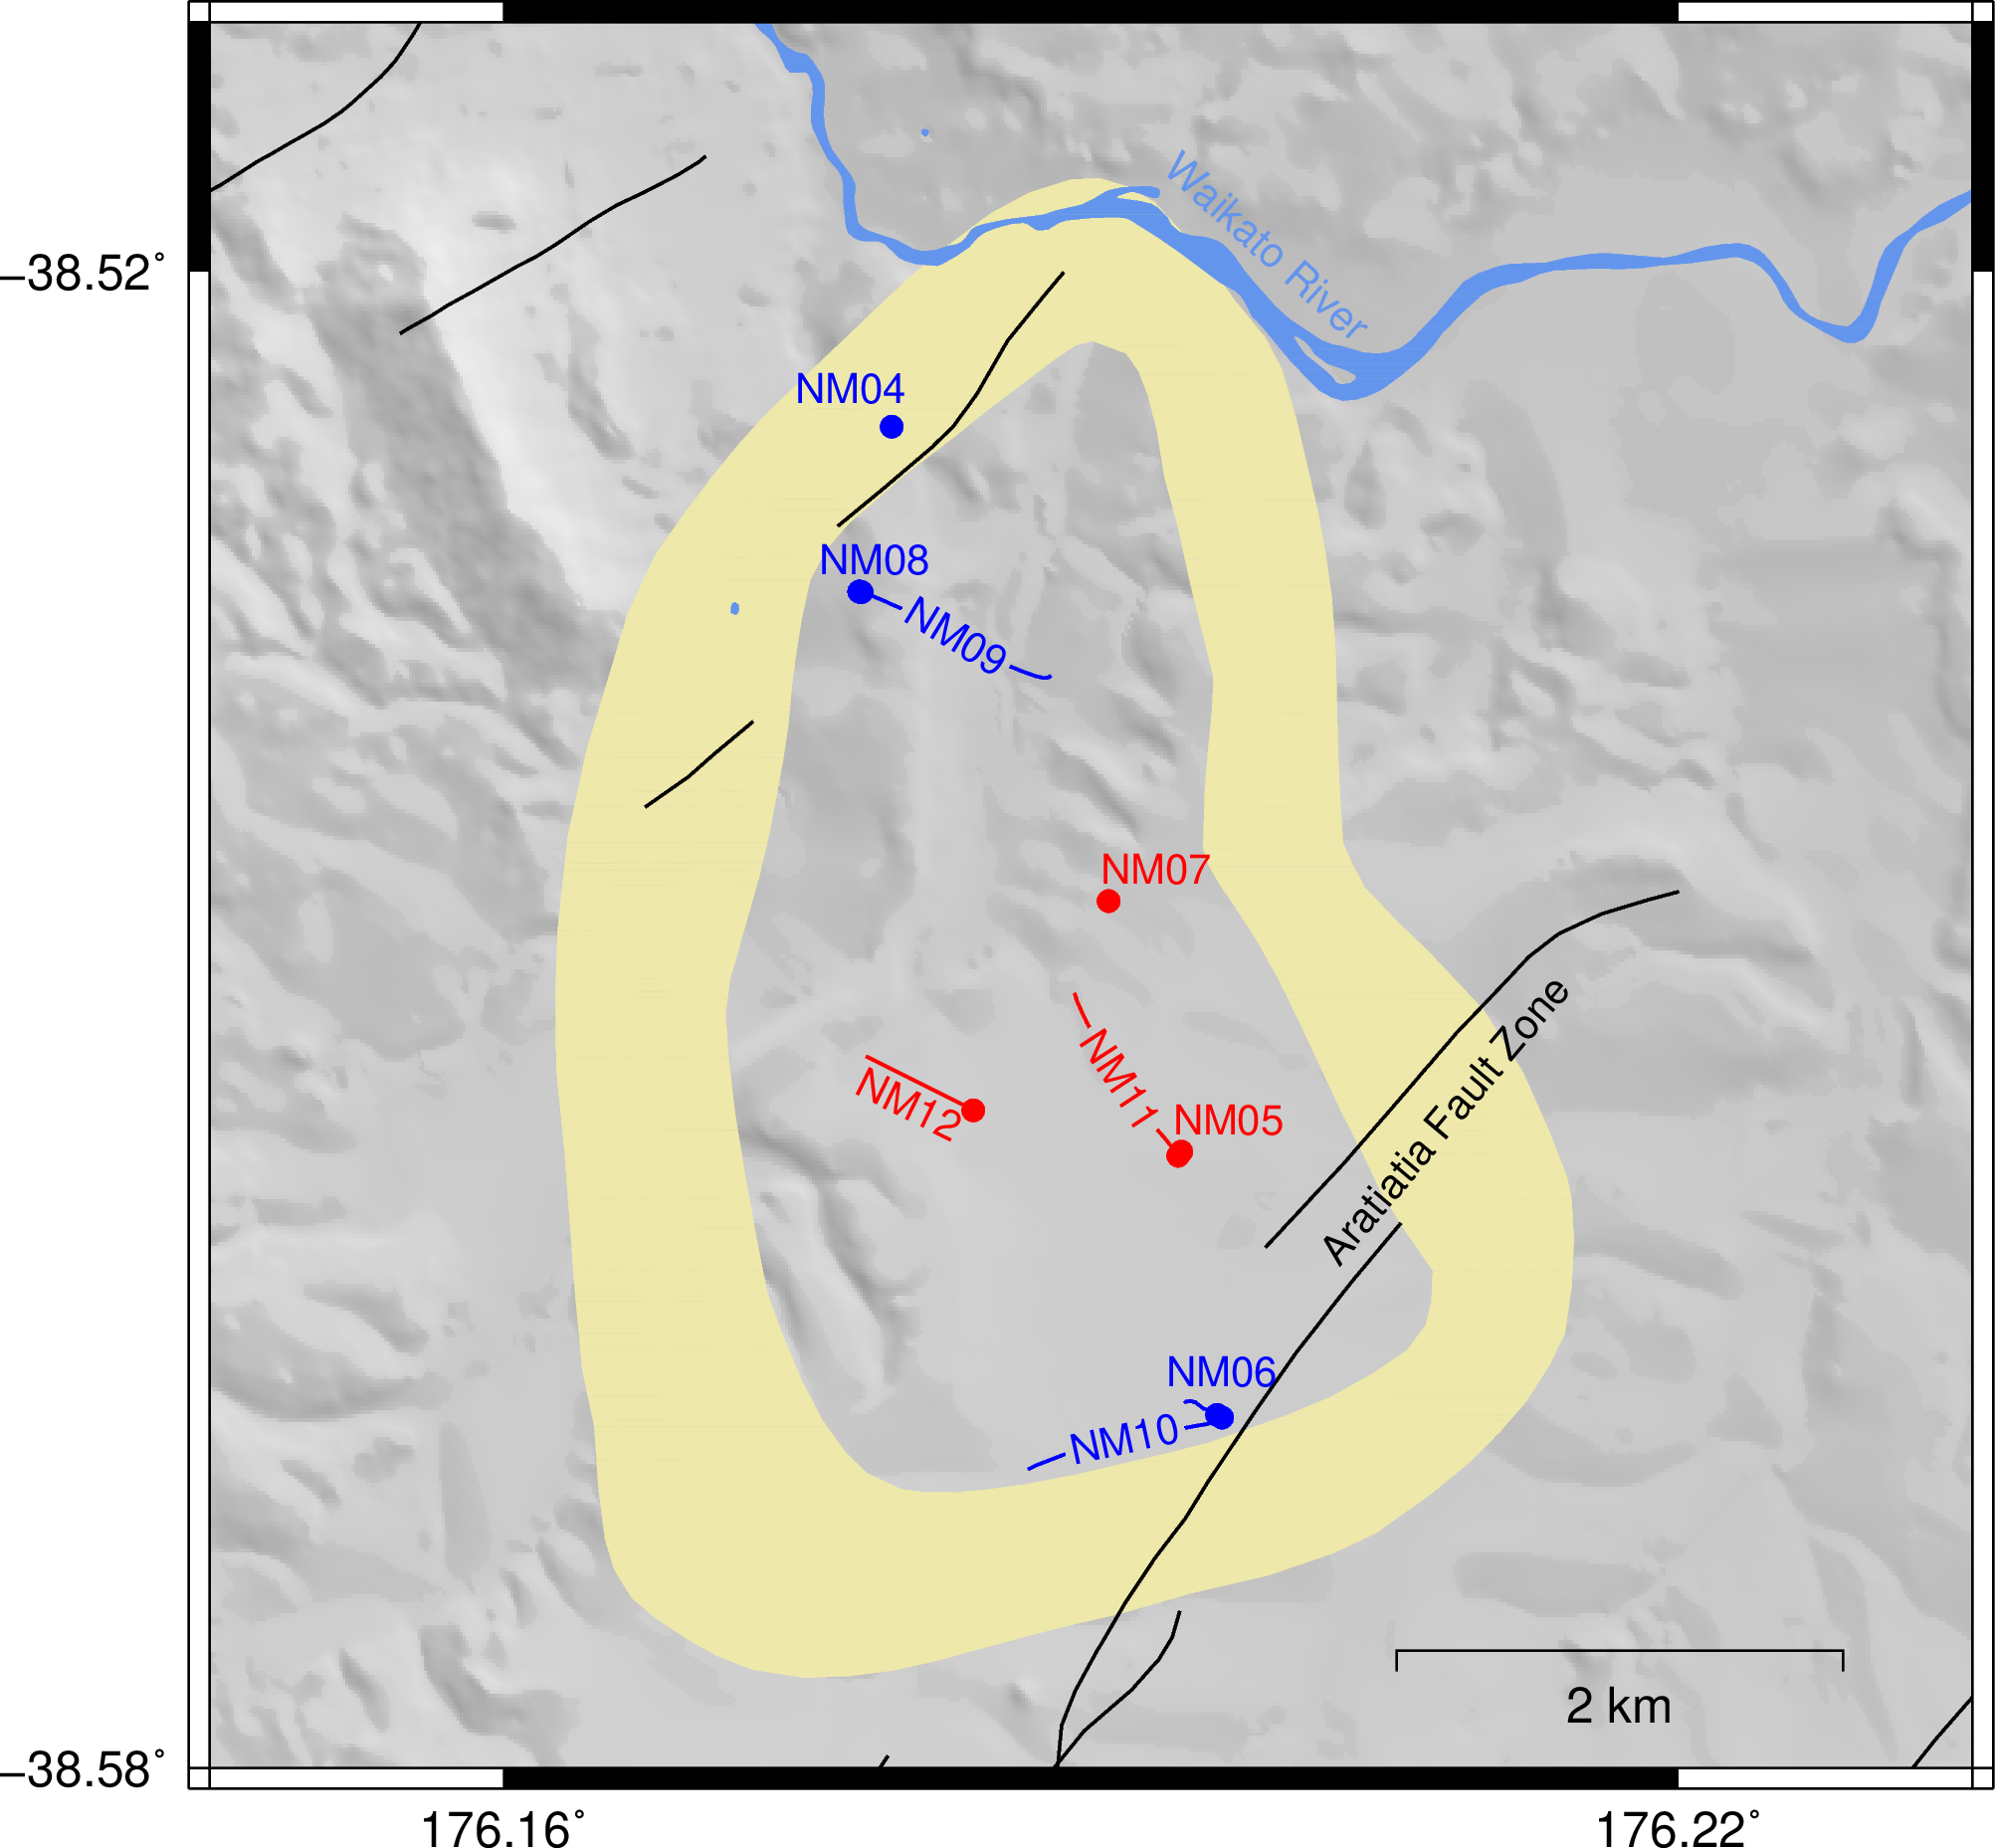
\includegraphics[width=0.70\columnwidth]{Chapter_1_Intro/figures/merc_Nga_overview_temps-wells_12-15_no_inset/merc_Nga_overview_temps-wells_12-15_no_inset_original}
\caption{{Overview of the Ngatamariki geothermal field. Injection wells are shown
in blue, production wells in red with dots representing the wellhead and
lines showing the surface projection of the well at depth. Wells NM04,
NM08, NM05 and NM07 are near vertical and, therefore, appear only as
dots in the figure.~ Active faults from the GNS Active Faults
Database~\protect\citet{AFDB} are shown in black. The most likely boundary
of the deep resource as published by~\protect\citet{Boseley_2010} based on
magnetotelluric surveys, is shown in yellow.
{\label{425195}}%
}}
\end{center}
\end{figure}\selectlanguage{english}

\begin{sidewaysfigure}[p]
\begin{center}
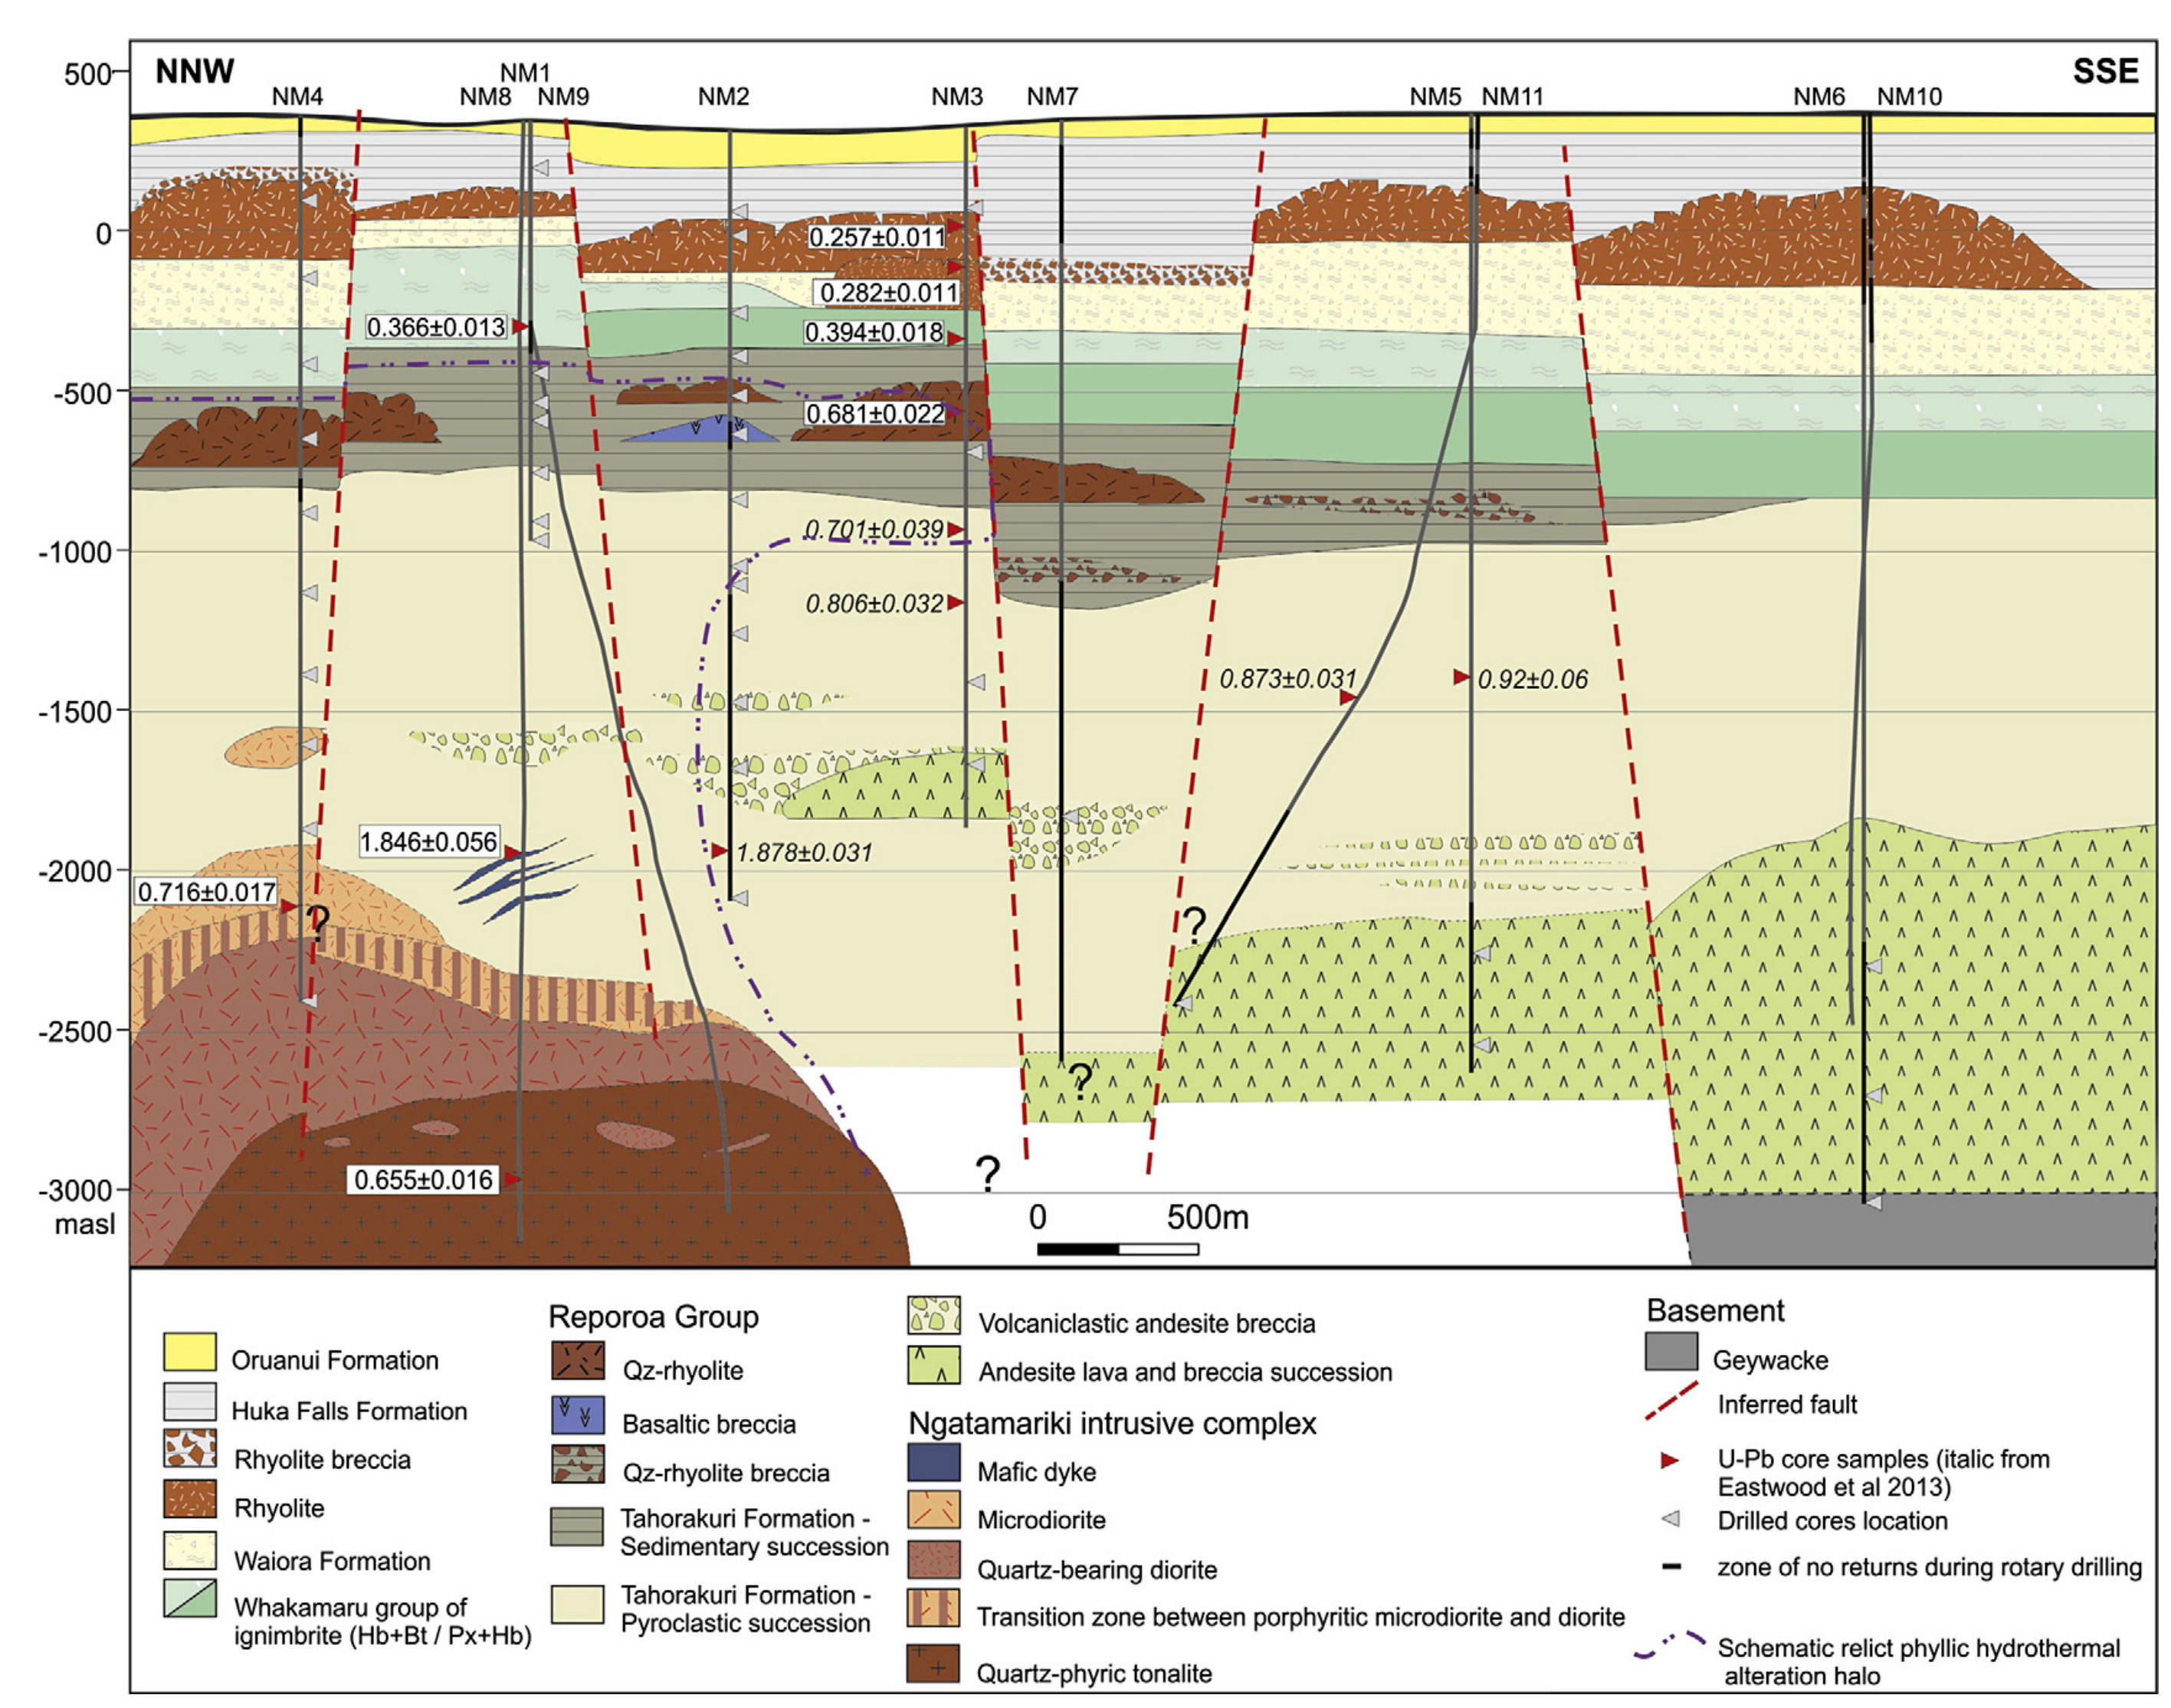
\includegraphics[width=0.7\textwidth,height=0.7\textheight,keepaspectratio]{Chapter_1_Intro/figures/Chamberfort_2014_fig3/Chamberfort_2014_fig3_original}
\caption{{Detailed geologic and structural context for the Ngatamariki geothermal
field from~\protect\citet{Chambefort_2014} including U-Pb dates (red triangles and
black text) and locations of core from each well. Question marks
correspond to contacts or faults which are consistent with the data from
the wells but which are not confirmed.
{\label{673646}}%
}}
\end{center}
\end{sidewaysfigure}

\subsubsection{Development}
Development at Ngatamariki began with the drilling of four deep exploration wells by the New Zealand government in 1984 \citep{Clearwater_2015}. Although these demonstrated the existence of a potentially viable resource, full-scale development for geothermal power was not undertaken until 2004 when Mercury (then known as Mighty River Power) partnered with the Tauhara No. 2 Trust, representing the local Maori landowners, to drill additional wells and eventually build the current, 82MWe power station \citep{Clearwater_2015}. Between June 2012 and February 2013 wells NM08, NM09 and NM10 were drilled as injection wells at the periphery of the deep reservoir. For each, a completion\slash{stimulation} test was conducted \citep{Clearwater_2015}. The Ngatamariki power plant was then brought online starting in April 2013 with gradually increasing flow rates until the reservoir reached a roughly stable state at around the start of 2015 (Figure \ref{953396}).

Mercury have identified three periods between 2012 and 2015 during which the relationship between injection and production parameters and seismicity is of particular interest. We have added an additional period which has been previously analyzed by MSc student Gabe Matson:
\begin{itemize}
  \item{NM08 Stimulation}
  
  From June 7 until July 10, 2012 (Figure \ref{953396}), northern injection well NM08 (Figure \ref{425195}) underwent a completion and stimulation test. Although low permeability was encountered during drilling, NM08 responded well to stimulation \citep{Clearwater_2015}. MSc student Gabe Matson analyzed this particular injection using similar techniques to what will be detailed in this work. Here we also analyze this period and compare our results to those obtained independently by Matson to check on our methodology.
  \item{NM09 Stimulation}
  
  From December 2012 until late January 2013 (Figure \ref{953396}) northern injection well NM09 (Figure \ref{425195}) also underwent completion and stimulation testing. NM09 responded positively to stimulation, although not as positively as NM08 and very little seismicity was initially detected \citep{Clearwater_2015}.
  \item{NM10 Drilling Losses and Stimulation}
  
  In July 2012 (Figure \ref{953396}), total fluid losses were encountered during drilling of southern injection well NM10 (Figure \ref{425195}). This was followed a month later by a completion and stimulation test, as at NM08 and NM09.
  \item{NM12 Drilling Losses}
  
  Similar to what occurred at NM10 in 2012, total fluid losses were incurred during the drilling of production well NM12 from June to September 2014 (Figure \ref{953396}).
\end{itemize}

In addition to these periods of interest, we will also investigate the seismic response to the plant startup at Ngatamariki (Figure \ref{953396}), which involved flow rates up to five-times greater than during the periods outlined above, and WHP of up to 2.0 MPa.\selectlanguage{english}

\begin{figure}[h!]
\begin{center}
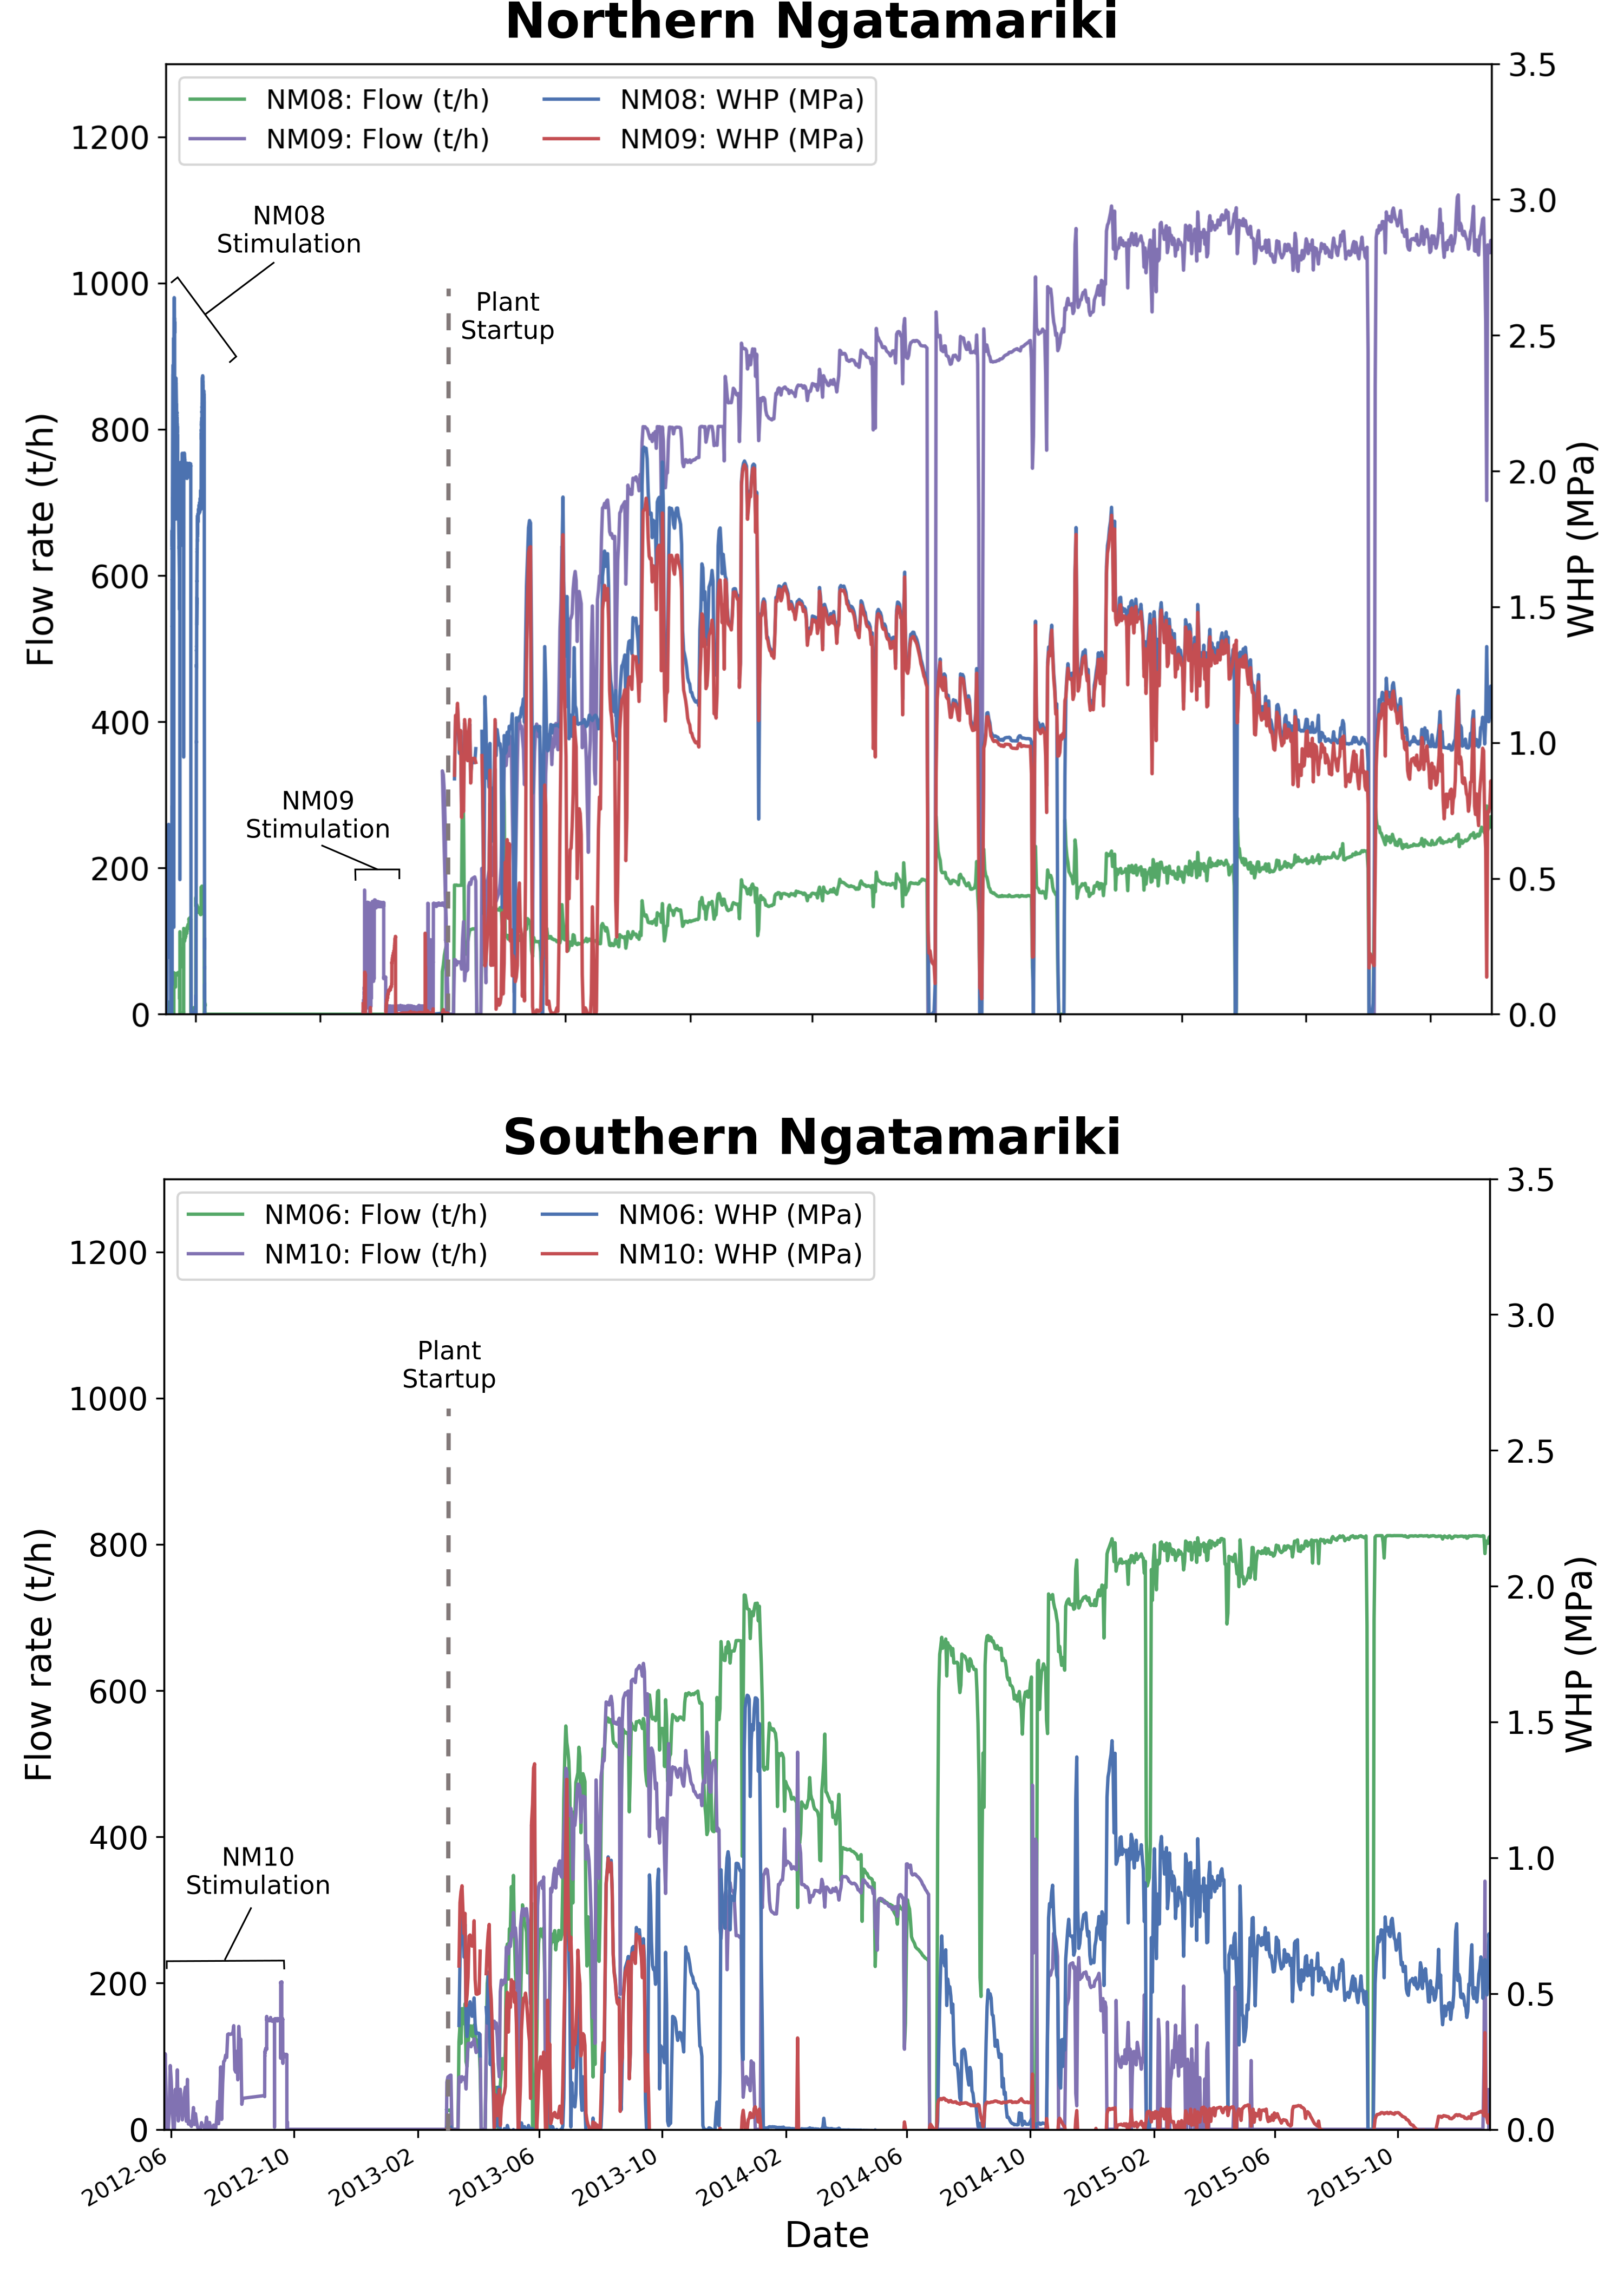
\includegraphics[width=0.84\columnwidth]{Chapter_1_Intro/figures/NgaN_ALL_flows_WHP/Ngatamariki_overview_Intro_original}
\caption{{Summary figure including the flow rates and wellhead pressures at each
of the four injection wells at Ngatamariki for 2012-2015 (separated into
northern and southern injection zones). The main periods of interest,
including the three completion\slash{stimulation} tests and the plant startup
are annotated. Drilling of NM12 occurred between June and September 2014, but is not annotated here as we have no flow data for that operation.
{\label{953396}}%
}}
\end{center}
\end{figure}

\subsubsection{Conceptual Model}
The hydrology at Ngatamariki consists of three semi-isolated aquifers at differing depths: the shallow aquifer at the surface, an intermediate aquifer above $\sim$500 m bsl, and the deep geothermal reservoir below that \citep{Boseley_2010,Chambefort_2016} (Figure \ref{813462}). Each of these aquifers is separated by an impermeable layer that, in the case of silicic volcanic rocks in the presence of weakly acidic fluids, is typically created by alteration to illite-smectite clay \citep{Boseley_2010}. These layers are normally diagnostic of geothermal reservoirs and are generally inferred from areas of low resistivity \citep[e.g.][]{Bibby_1995} and conductive portions of well temperature profiles \citep{Grant_2011}. The deep reservoir at Ngatamariki is isolated from the intermediate aquifer by a clay cap that ranges in thickness from \textgreater1000 m at the northern periphery to practically nonexistent between monitoring\slash{exploration} wells NM2 and NM3, where \citet{Boseley_2010} have inferred a hydrologic connection to the intermediate aquifer called `the leak' (Figure \ref{813462}). This point also marks the center of the `upflow', which refers to the area of upward convection within a geothermal system and is commonly a target for production wells \citep{Grant_2011}. Reservoir permeability in the TVZ is dominated by existing faults and fractures, as the matrix permeability of the typical volcanic rocks is low \citep{Grant_2011,Cant_2018}. This is certainly the case at Ngatamariki, where the Tahorakuri and Rotokawa Andesite that host the reservoir have been shown to be highly fractured in image logs \citep{nm09_report,nm10_report,massiot_2012} and fracture-dominated flow is assumed when modeling the reservoir \citep[e.g.][]{Quinao_2018}.\selectlanguage{english}

\begin{sidewaysfigure}[p]
\begin{center}
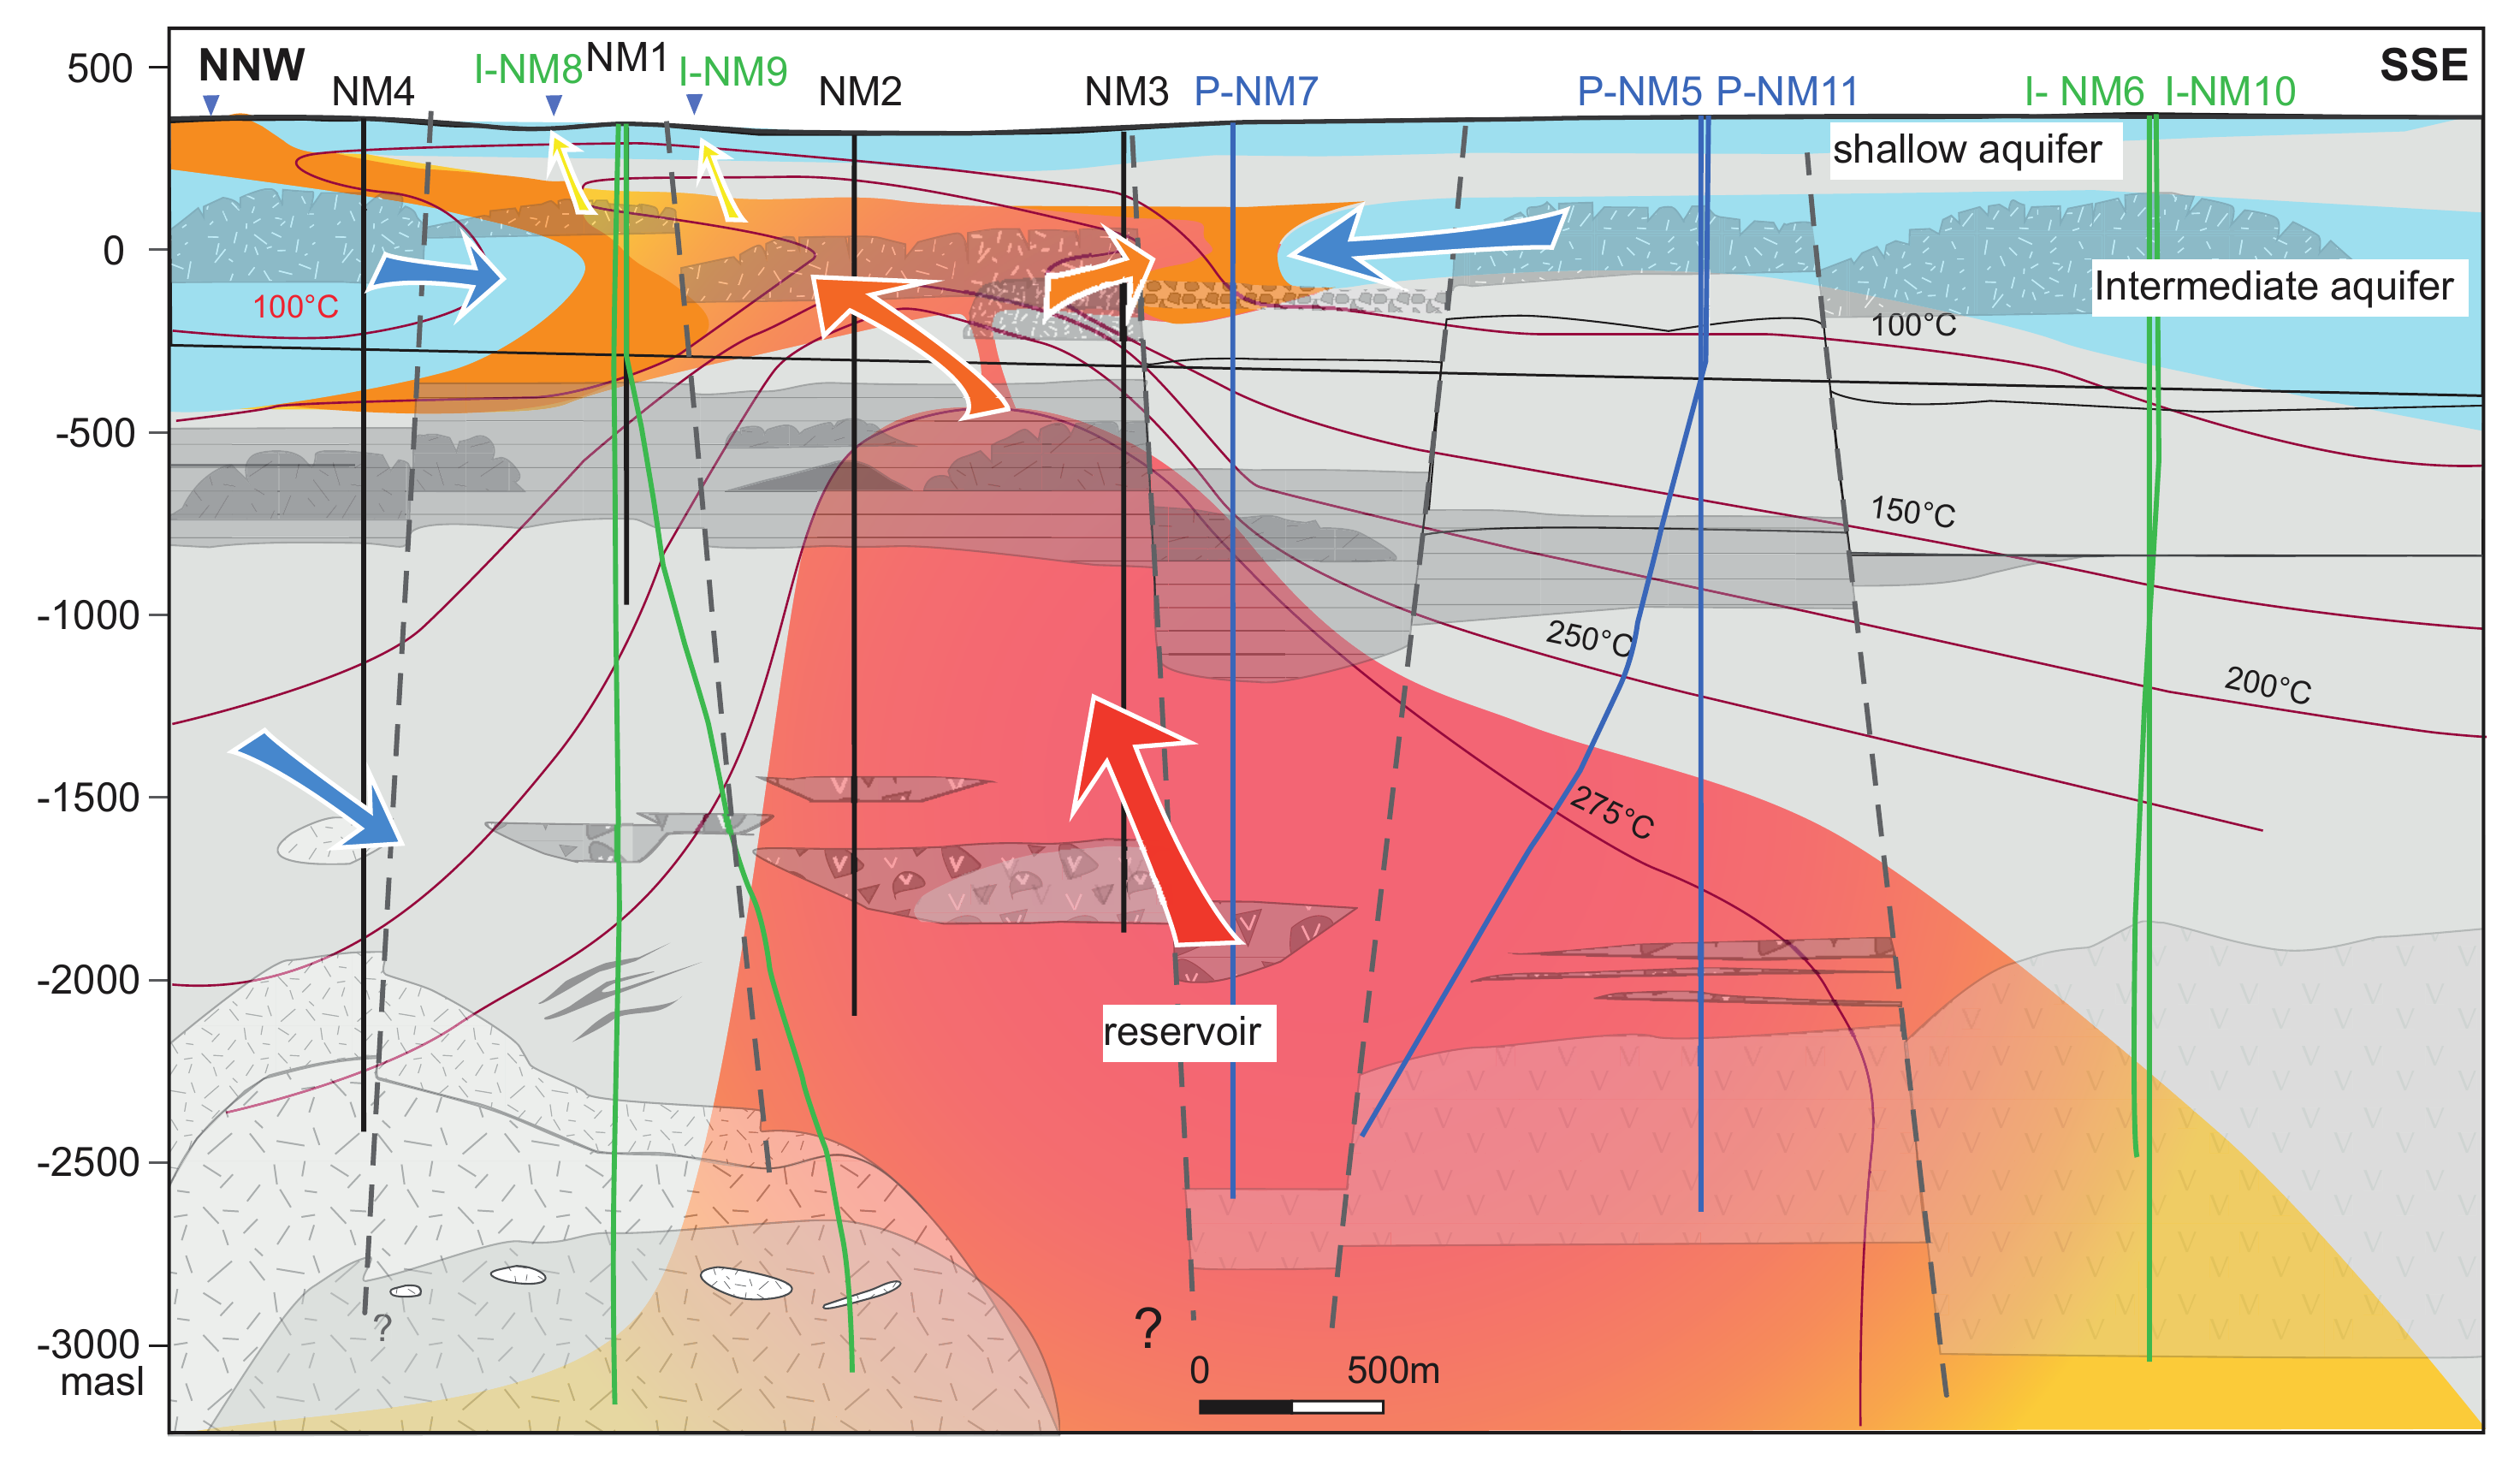
\includegraphics[width=0.7\textwidth,height=0.7\textheight,keepaspectratio]{Chapter_1_Intro/figures/Chamerfort_2015_fig9_model/Chamberfort_2015_fig9_model_original}
\caption{{Ngatamariki conceptual model proposed by~\protect\citet{Boseley_2010} overlain on
the geologic cross section in Figure~{\ref{673646}}
by~\protect\citet{Chambefort_2016}. In this figure, green wells are injection wells
and blue are production. Note that, for most figures in this work, blue
wells will signify injection and red production. The main upflow at
Ngatamariki is located between wells NM2 and NM3, in the northern part
of the reservoir. Arrows indicate flow direction with the color
signifying the relative temperature of the fluid (red=hot, blue=cold).
Maroon lines are isotherms modeled from well temperature profiles.
{\label{813462}}%
}}
\end{center}
\end{sidewaysfigure}

Nearly all of the produced fluid at Ngatamariki is reinjected into the reservoir. In order to maintain flexibility with regard to reservoir management, there are two reinjection fields (green wells, Figures \ref{425195},\ref{813462}, blue lines in all other figures) to the north and south of the central production field (blue lines, Figure \ref{813462}, red lines in all other figures). The distribution of injection between the two fields varies with time in response to changes in the reservoir and degradation of wells. Generally, more fluid is injected into the northern injection zone than the southern. Well NM09, in the north, is the dominant injection well for the entire field (currently \textgreater1000 t/h). However, the heterogeneity of the permeability structure is considerable. Well NM08 is far less permeable than NM09, although they are separated by only hundreds of meters at reservoir depth \citep{Clearwater_2015}. Permeability also varies substantially with depth, particularly in the northern injection zone where the wells intersect the diorite\slash{tonalite} intrusive body, which has a very low matrix permeability \citep{Cant_2018}. While all of the wells drilled at Ngatamariki can be considered to be highly-fractured \citep{nm09_report,nm10_report,massiot_2012}, only a portion of these fractures are open and able to accept fluid upon injection or production (we refer to these high-permeability areas as feedzones). Therefore, the most permeable wells in the field are those that intersect active fracture zones that have a high likelihood of being open and not filled with minerals. Such high-permeability fracture zones are intersected at NM09, NM06 and NM10, but not at NM08 \citep{nm09_report,nm10_report,massiot_2012} and is reflected in the wellhead pressures measured at each well.

In the southern injection zone, radioactive tracer tests have revealed well NM10 to be well-connected, hydrologically, to the southern production well NM5 \citep{buscarlet_2015}. As such a connection produces a loss in entropy (cooler water is extracted), and therefore a loss in power generation capacity at the plant, NM10 was phased out as an injection well by early 2015 (Figure \ref{953396}). The excess injection in the southern part of the field was then accomodated by well NM06 (Figure \ref{425195}).

\subsection{Rotokawa}
\subsubsection{Geology}
The Rotokawa geothermal field is located $\sim$7 km south of Ngatamariki. The resource, as defined by the resistivity boundaries shown in Figure \ref{838185} \citep{Risk_2000}, measures approximately 4 km in diameter. The surface projection of the resource sits astride the Waikato River and all of the development to-date has occurred south of the river. Rotokawa is also a naturally-fractured, liquid-dominated reservoir, but the maximum temperatures encountered at depth are the highest measured in the entire TVZ (337\textdegree C in well RK22). Given their close proximity, the geology at Rotokawa is very similar to that of Ngatamariki, although the heterogeneity of relatively young TVZ volcanic deposits and active faulting have led to certain differences. Most importantly, while the Ngatamariki reservoir is hosted in Rotokawa Andesite and Tahorakuri Formation rocks, the shallower depth to the basement at Rotokawa (up to 1700 m bsl) means that much of the reservoir is hosted in Torlesse Greywacke (Figure \ref{599670}) \citep{wallis2013,McNamara_2016}. The rest of the Rotokawa reservoir is mostly hosted in Rotokawa Andesite which reaches thicknesses of 1500 m and is laterally coherent across the field, although the shallower parts of the production field (red wells, Figure \ref{838185}) are hosted in variable thicknesses of Tahorakuri Formation and Wairakei Ignimbrite (part of the Whakamaru Group; \textless0.35 Ma age) \citep{McNamara_2016}. At Rotokawa, there is no analog to the intrusive complex intersected in wells NM04, NM08 and NM09 at Ngatamariki.

The regional NE-SW structural grain still describes the first-order structure at Rotokawa, with the Aratiatia Fault Zone cutting across northwest corner of the field (Figure \ref{838185}) and three NE-SW-striking faults dividing the reservoir at depth: the \acrfull{PFF}, \acrfull{CFF} and \acrfull{IFF} (Figure \ref{599670}) \citep{wallis2013}. Each of these faults is inferred from vertical offsets in the basement greywacke and Rotokawa Andesite observed from well cuttings, microseismic locations and radioactive tracer returns between wells \citep{Sewell_2015,Addison_2017stanford,wallis2013}, but they are not observed to offset the overlying units \citep{wallis2013}.\selectlanguage{english}

\begin{figure}[h!]
\begin{center}
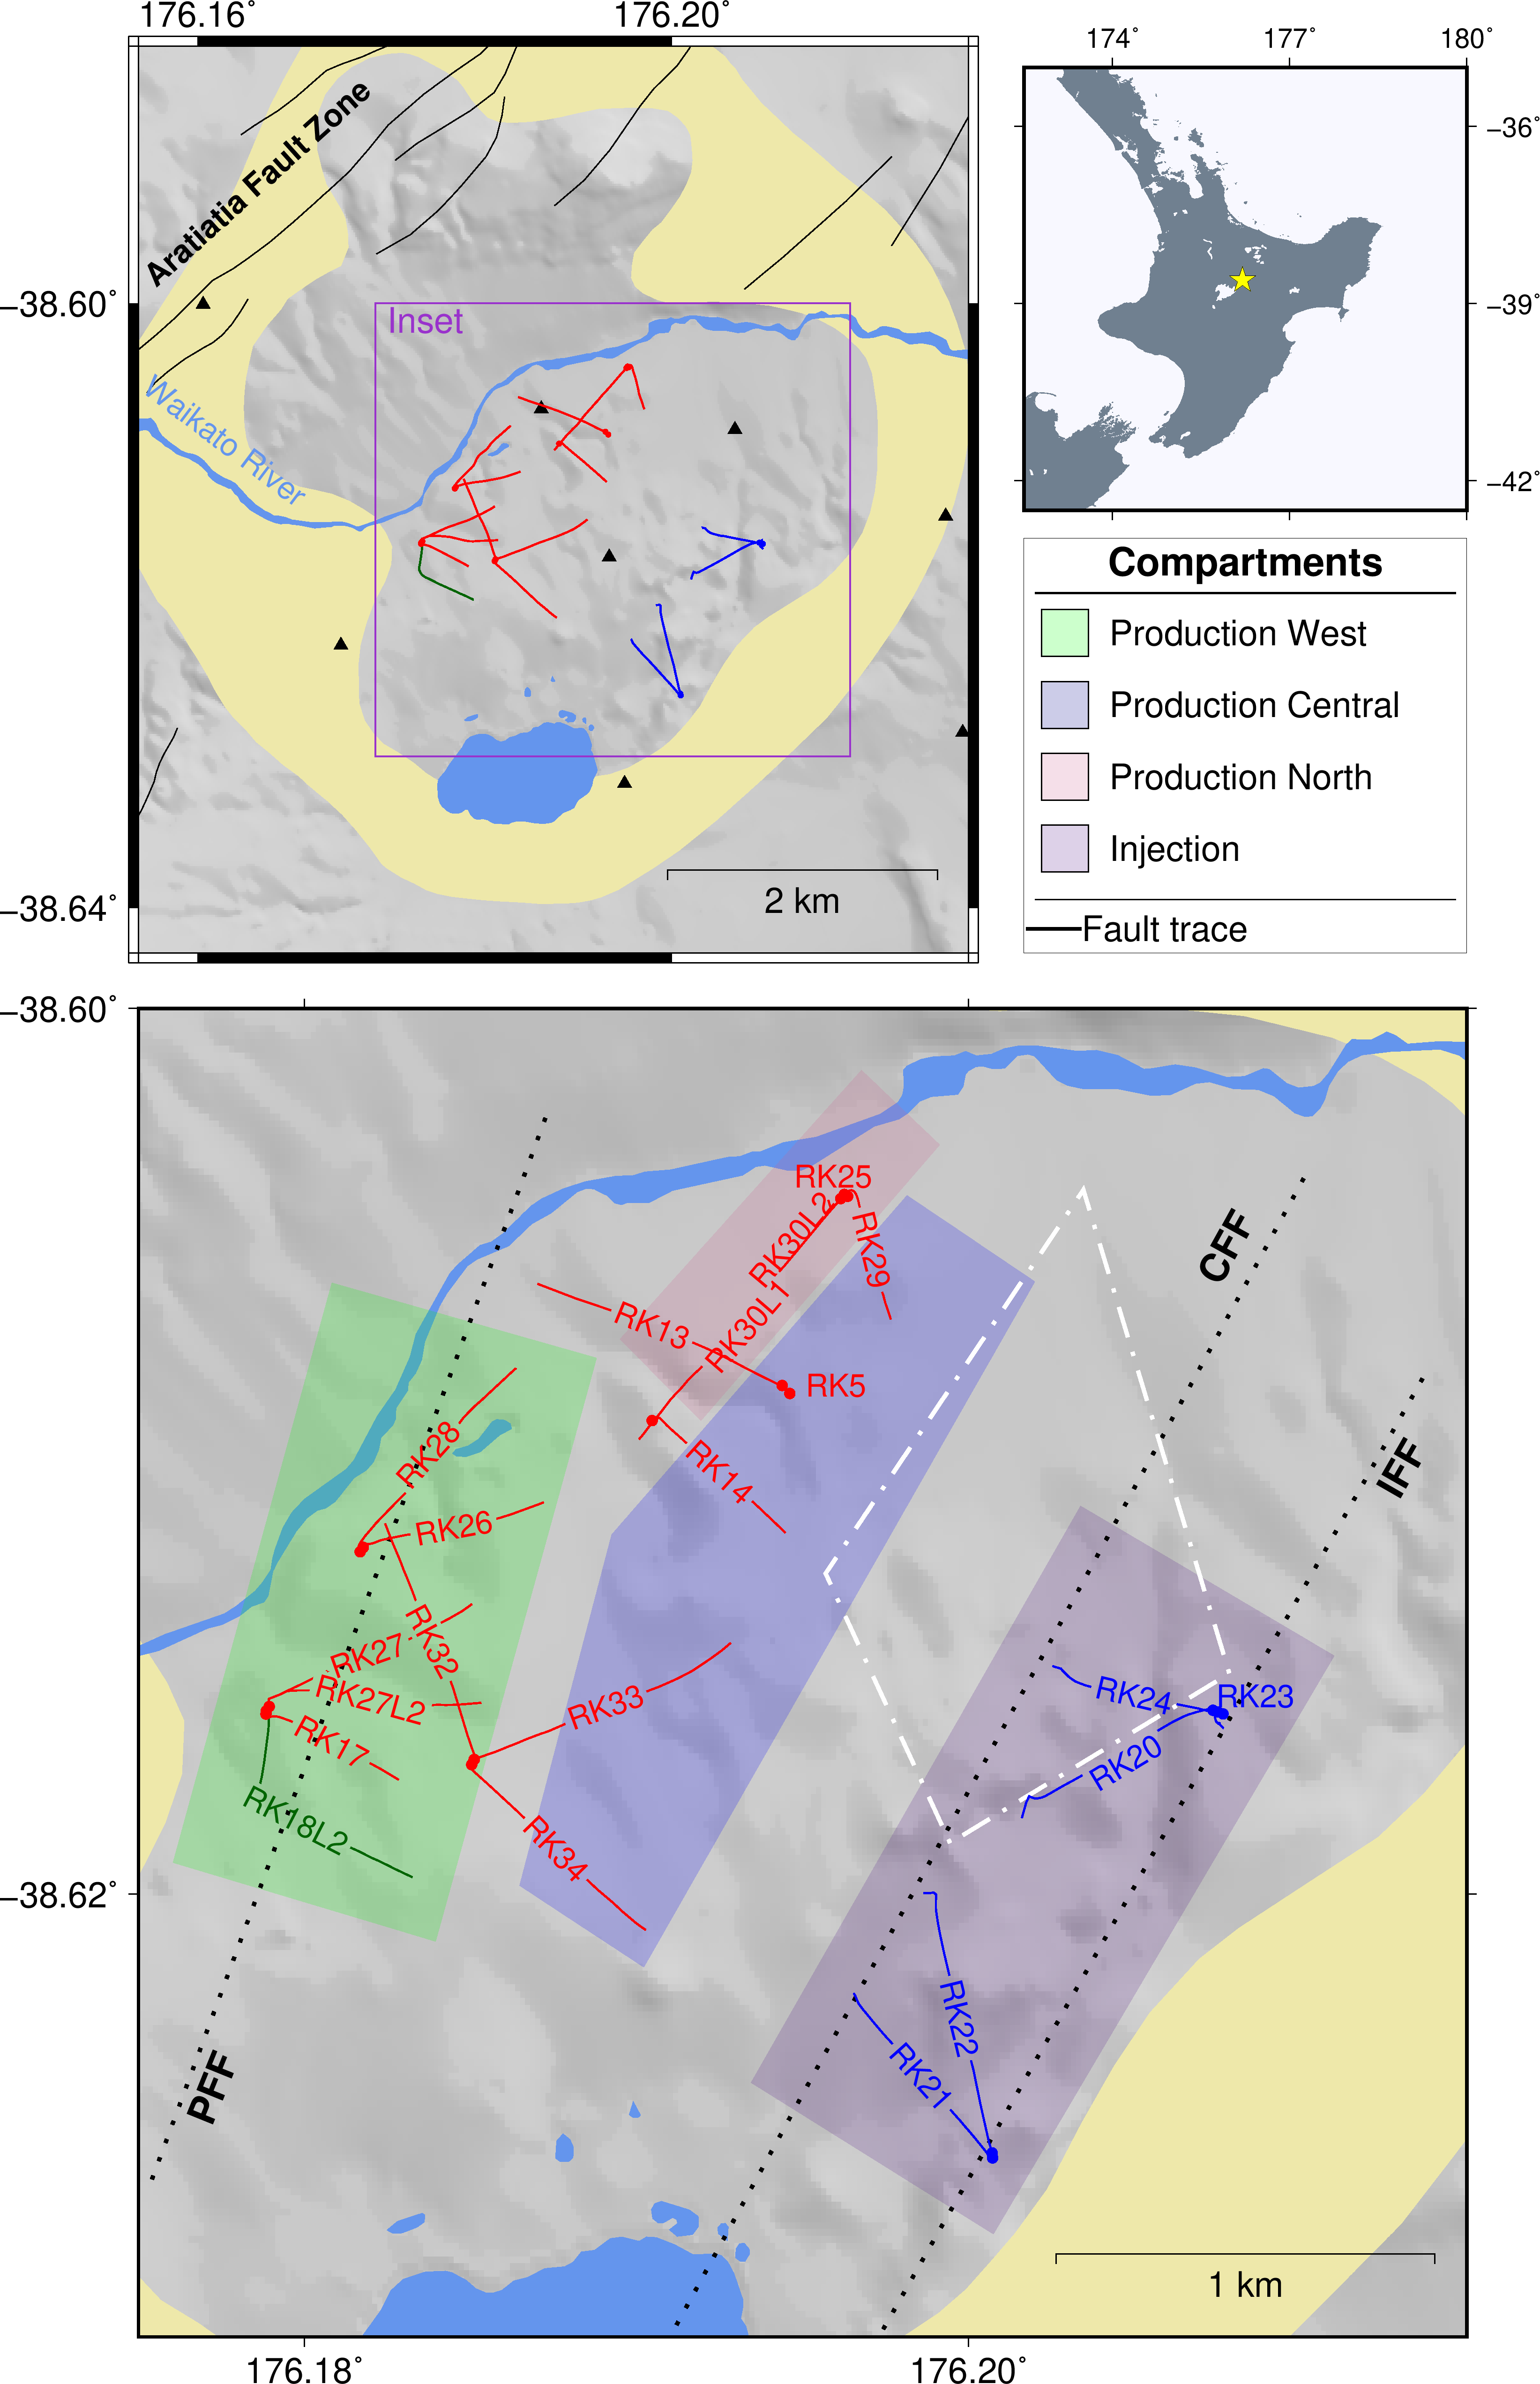
\includegraphics[width=1.00\columnwidth]{Chapter_1_Intro/figures/Rotokawa_overview_Intro/merc_Rot_overview_struct_inset_NI_compartments_original}
\caption{{Overview of the Rotokawa geothermal field. The top right panel shows the
location of the field on the North Island of New Zealand (yellow star).
The top left panel shows the resistivity boundary of the field in yellow
and injection and production wells in blue and red, respectively. Solid
black lines are active faults. The lower panel shows a closeup of the
field, with the well names labeled and the three known faults (PFF, CFF,
IFF) shown as black dotted lines. The white dot-dashed line shows the
extent of significant seismicity from 2008-2012, as reported
by~\protect\citet{Sherburn_2015}. There are four known compartments in the Rotokawa
reservoir shown as colored polygons. Each is semi-isolated from the
others by either a permeability contrast or impermeable barrier (i.e. a
fault). The production field comprises three compartments, the west,
central and north (green, blue and red, respectively). The injection
field is shaded in purple and is a separate compartment.
{\label{838185}}%
}}
\end{center}
\end{figure}\selectlanguage{english}

\begin{sidewaysfigure}[p]
\begin{center}
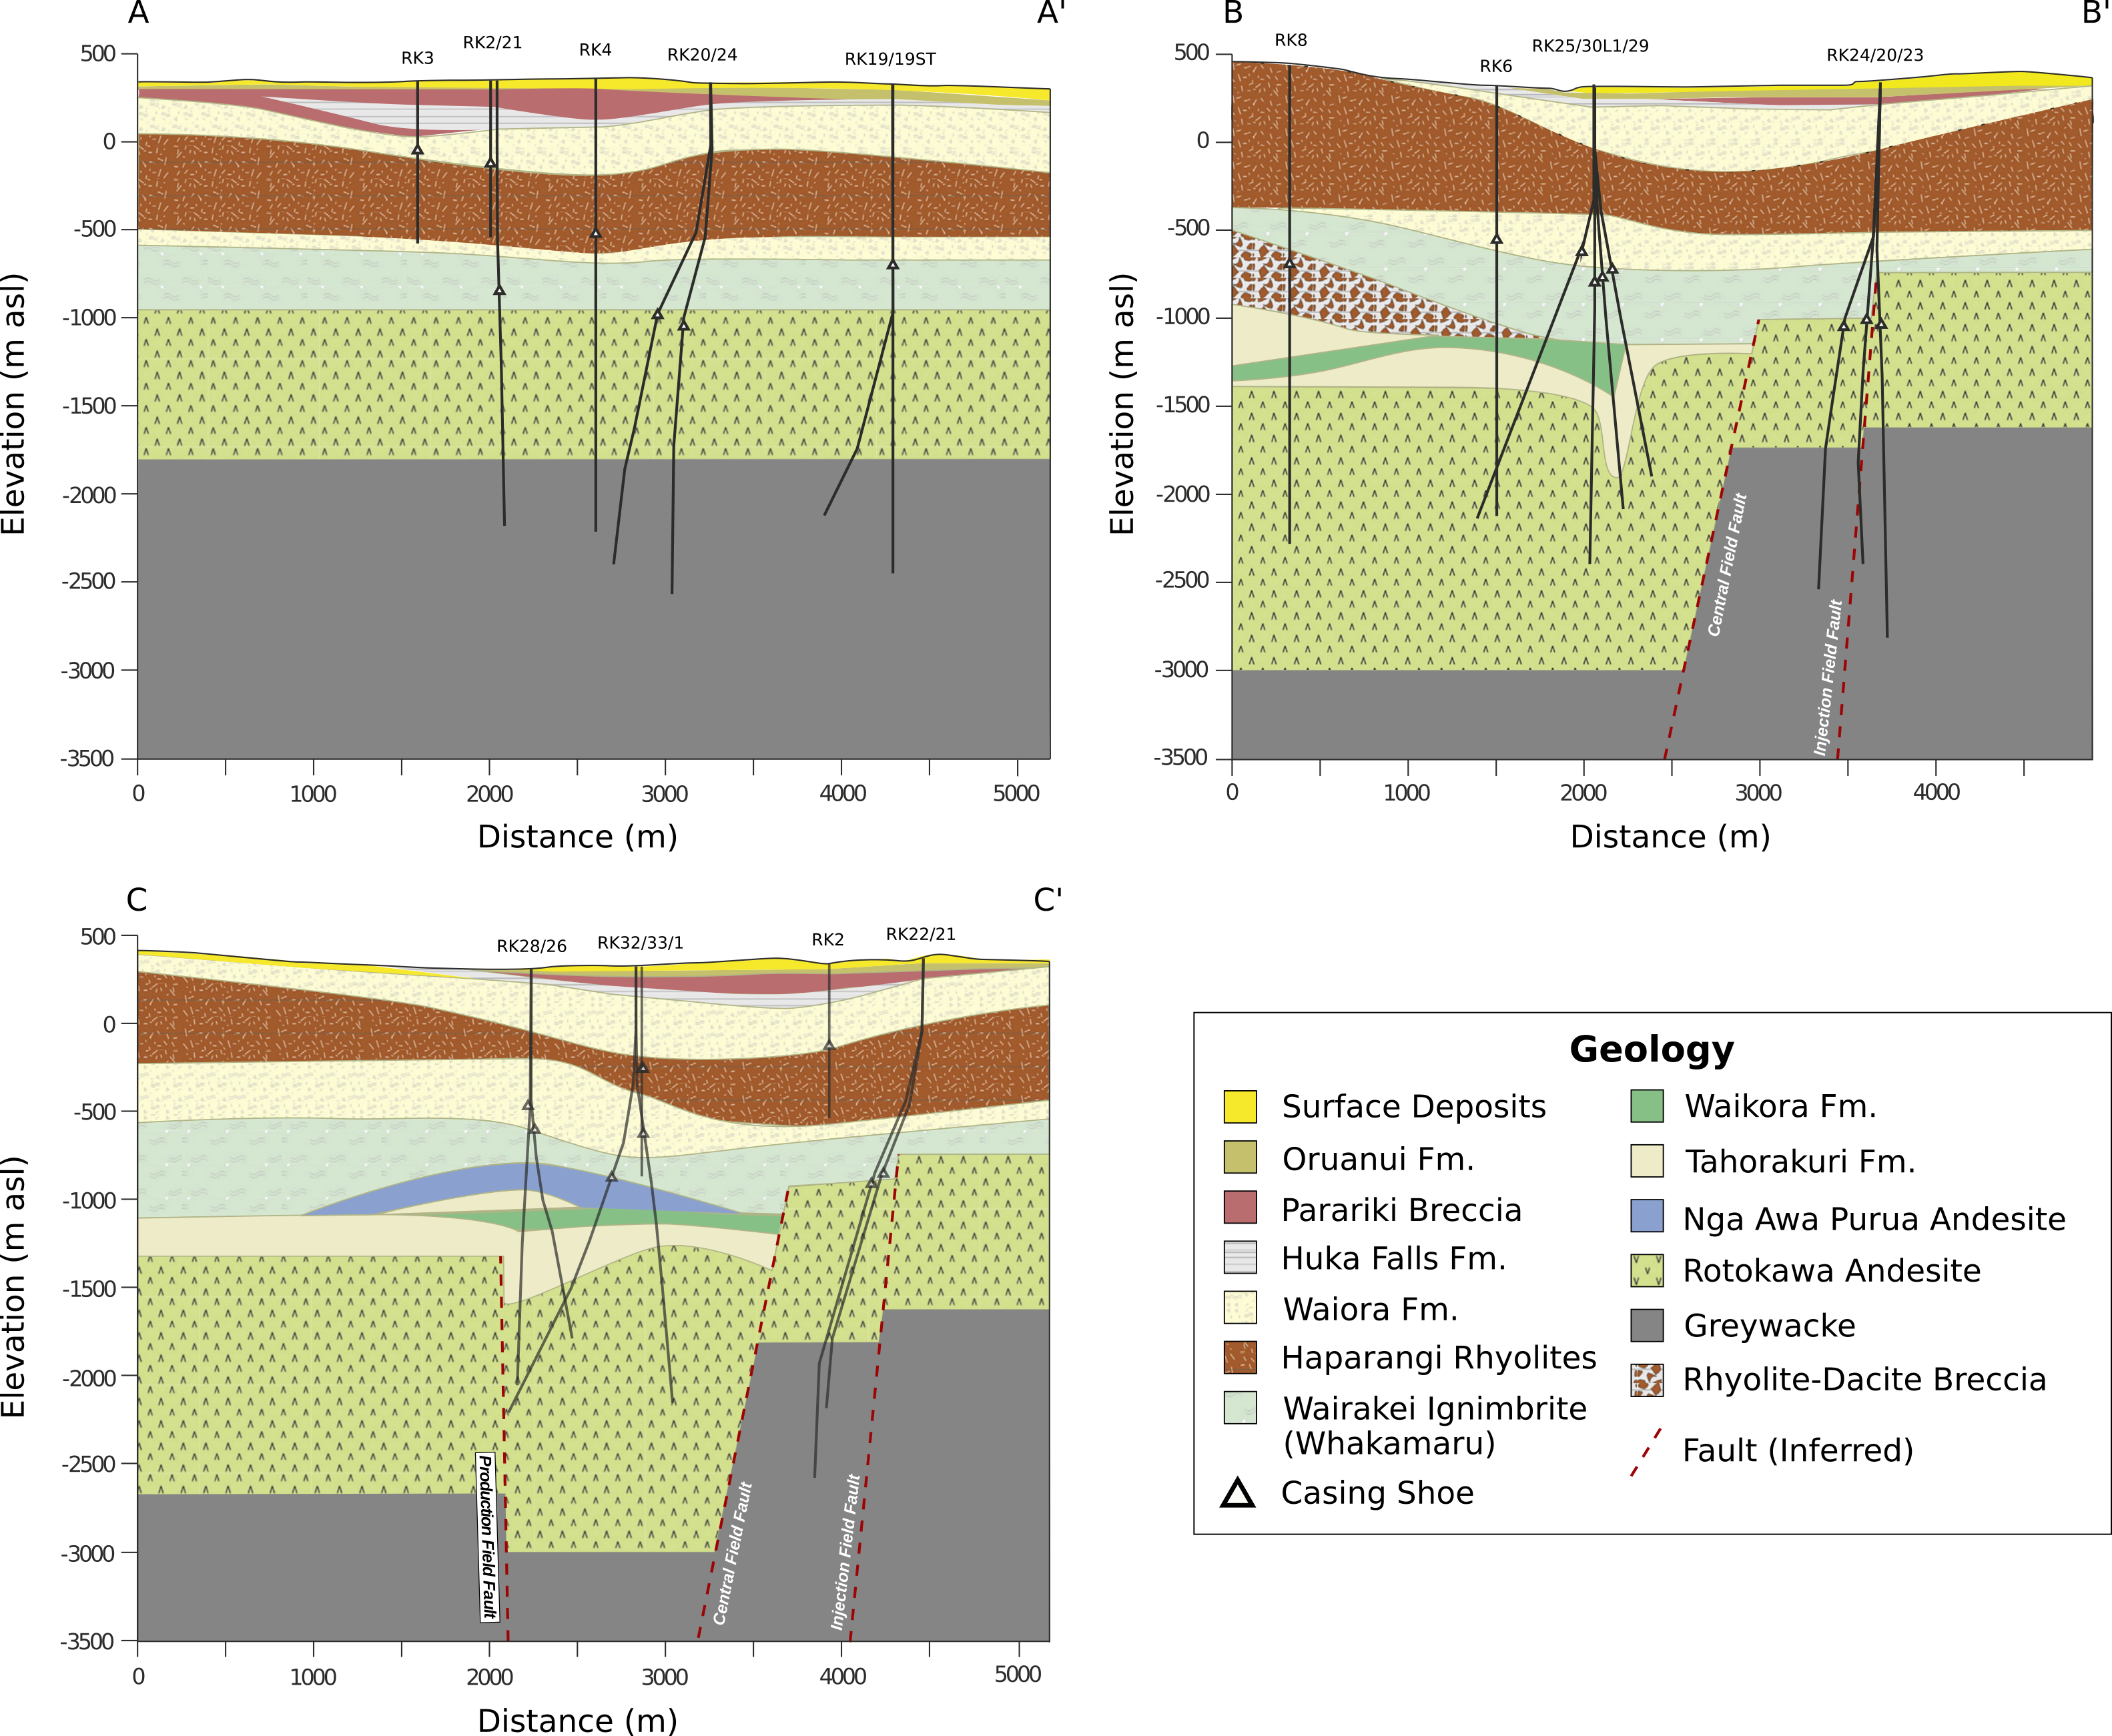
\includegraphics[width=0.7\textwidth,height=0.7\textheight,keepaspectratio]{Chapter_1_Intro/figures/Rotokawa_geology_11-20/Rotokawa_geology_11-20_original}
\caption{{Three selected cross-sections showing the geology of the Rotokawa
geothermal field (modified from~\protect\citet{Sewell_2015} to correspond to
Figure {\ref{673646}})
{\label{599670}}%
}}
\end{center}
\end{sidewaysfigure}

\subsubsection{Development}
As at Ngatamariki, resource characterization at Rotokawa began with exploratory drilling by the New Zealand government, which confirmed the existence of the \textgreater300\textdegree C resource \citep{Sewell_2015,McNamara_2016}. The Rotokawa binary plant (RKA) was installed in 1997 with a capacity of 24 MWe. During this phase of development, production and injection both occurred within the modern production field, with injection taking place between 500 and 1000 m depth \citep{Sewell_2015}. In 2000, production was increased to 34 MWe and the shallow injection was moved to deeper wells on the southwest periphery of the production field (RK16, RK18) (Figure \ref{838185}). In 2007, the Rotokawa Joint Venture (Tauhara No. 2 Trust and Mercury) were granted consents to increase development at Rotokawa with the addition of the 138 MWe Nga Awa Purua (NAP) triple-flash plant, which was comissioned in 2010 \citep{Sewell_2015}. With the drilling of wells RK19-RK30, the management strategy was shifted so that deep injection occurred to the southeast at wells RK20-RK24 and production came from the wells in the already-developed portions of the field (Figure \ref{838185}) \citep{Sewell_2015,McNamara_2016}. Requirements for further production prompted the drilling of wells RK32-RK34 following the startup of NAP (Figure \ref{838185}).

During the 2012-2015 dataset presented in this work, there were four main periods of interest identified by Mercury from a reservoir management perspective. The periods were:
\begin{itemize}
  \item{RK24 Injectivity Decline}
  
  Following NAP startup, it was determined from radioactive tracer returns that the southern injection wells, specifically RK21, were producing rapid returns at the southern production wells \citep{addison2015rotokawa}. Injection was moved to northern injection well RK24 but within six months II had begun to decline in the well (Figure \ref{701773}). Mercury have identified this as a time period of interest where patterns of seismicity may be able to inform the reason for this injectivity decline.
  \item{Switch of Injection: RK24-RK23}
  
  Given the II decline noted above, Mercury decided to shift some injection away from RK24 and into RK23 in June 2014. Mercury are interested in knowing if this produced an accompanying shift in seismicity as well (Figure \ref{701773}).
  \item{RK34 Drilling Losses}
  
  As with NM10 at Ngatamariki, total losses were incurred during the drilling of make-up production well RK34 from September to November 2014. It may be that such losses would trigger seismicity, which may be more easily identified in the less-seismically-active production field where RK34 was drilled.
  \item{Plant Shutdowns and Startups}
  
  For prior periods (i.e. before 2012), swarms of seismicity occurred in response to plant shutdowns and startups (typically related to maintenance). These swarms have been attributed to transient pressure changes in the reservoir \citep{Sherburn_2015}, and Mercury have identified future plant shutdowns as periods of seismic interest.
\end{itemize}\selectlanguage{english}

\begin{figure}[h!]
\begin{center}
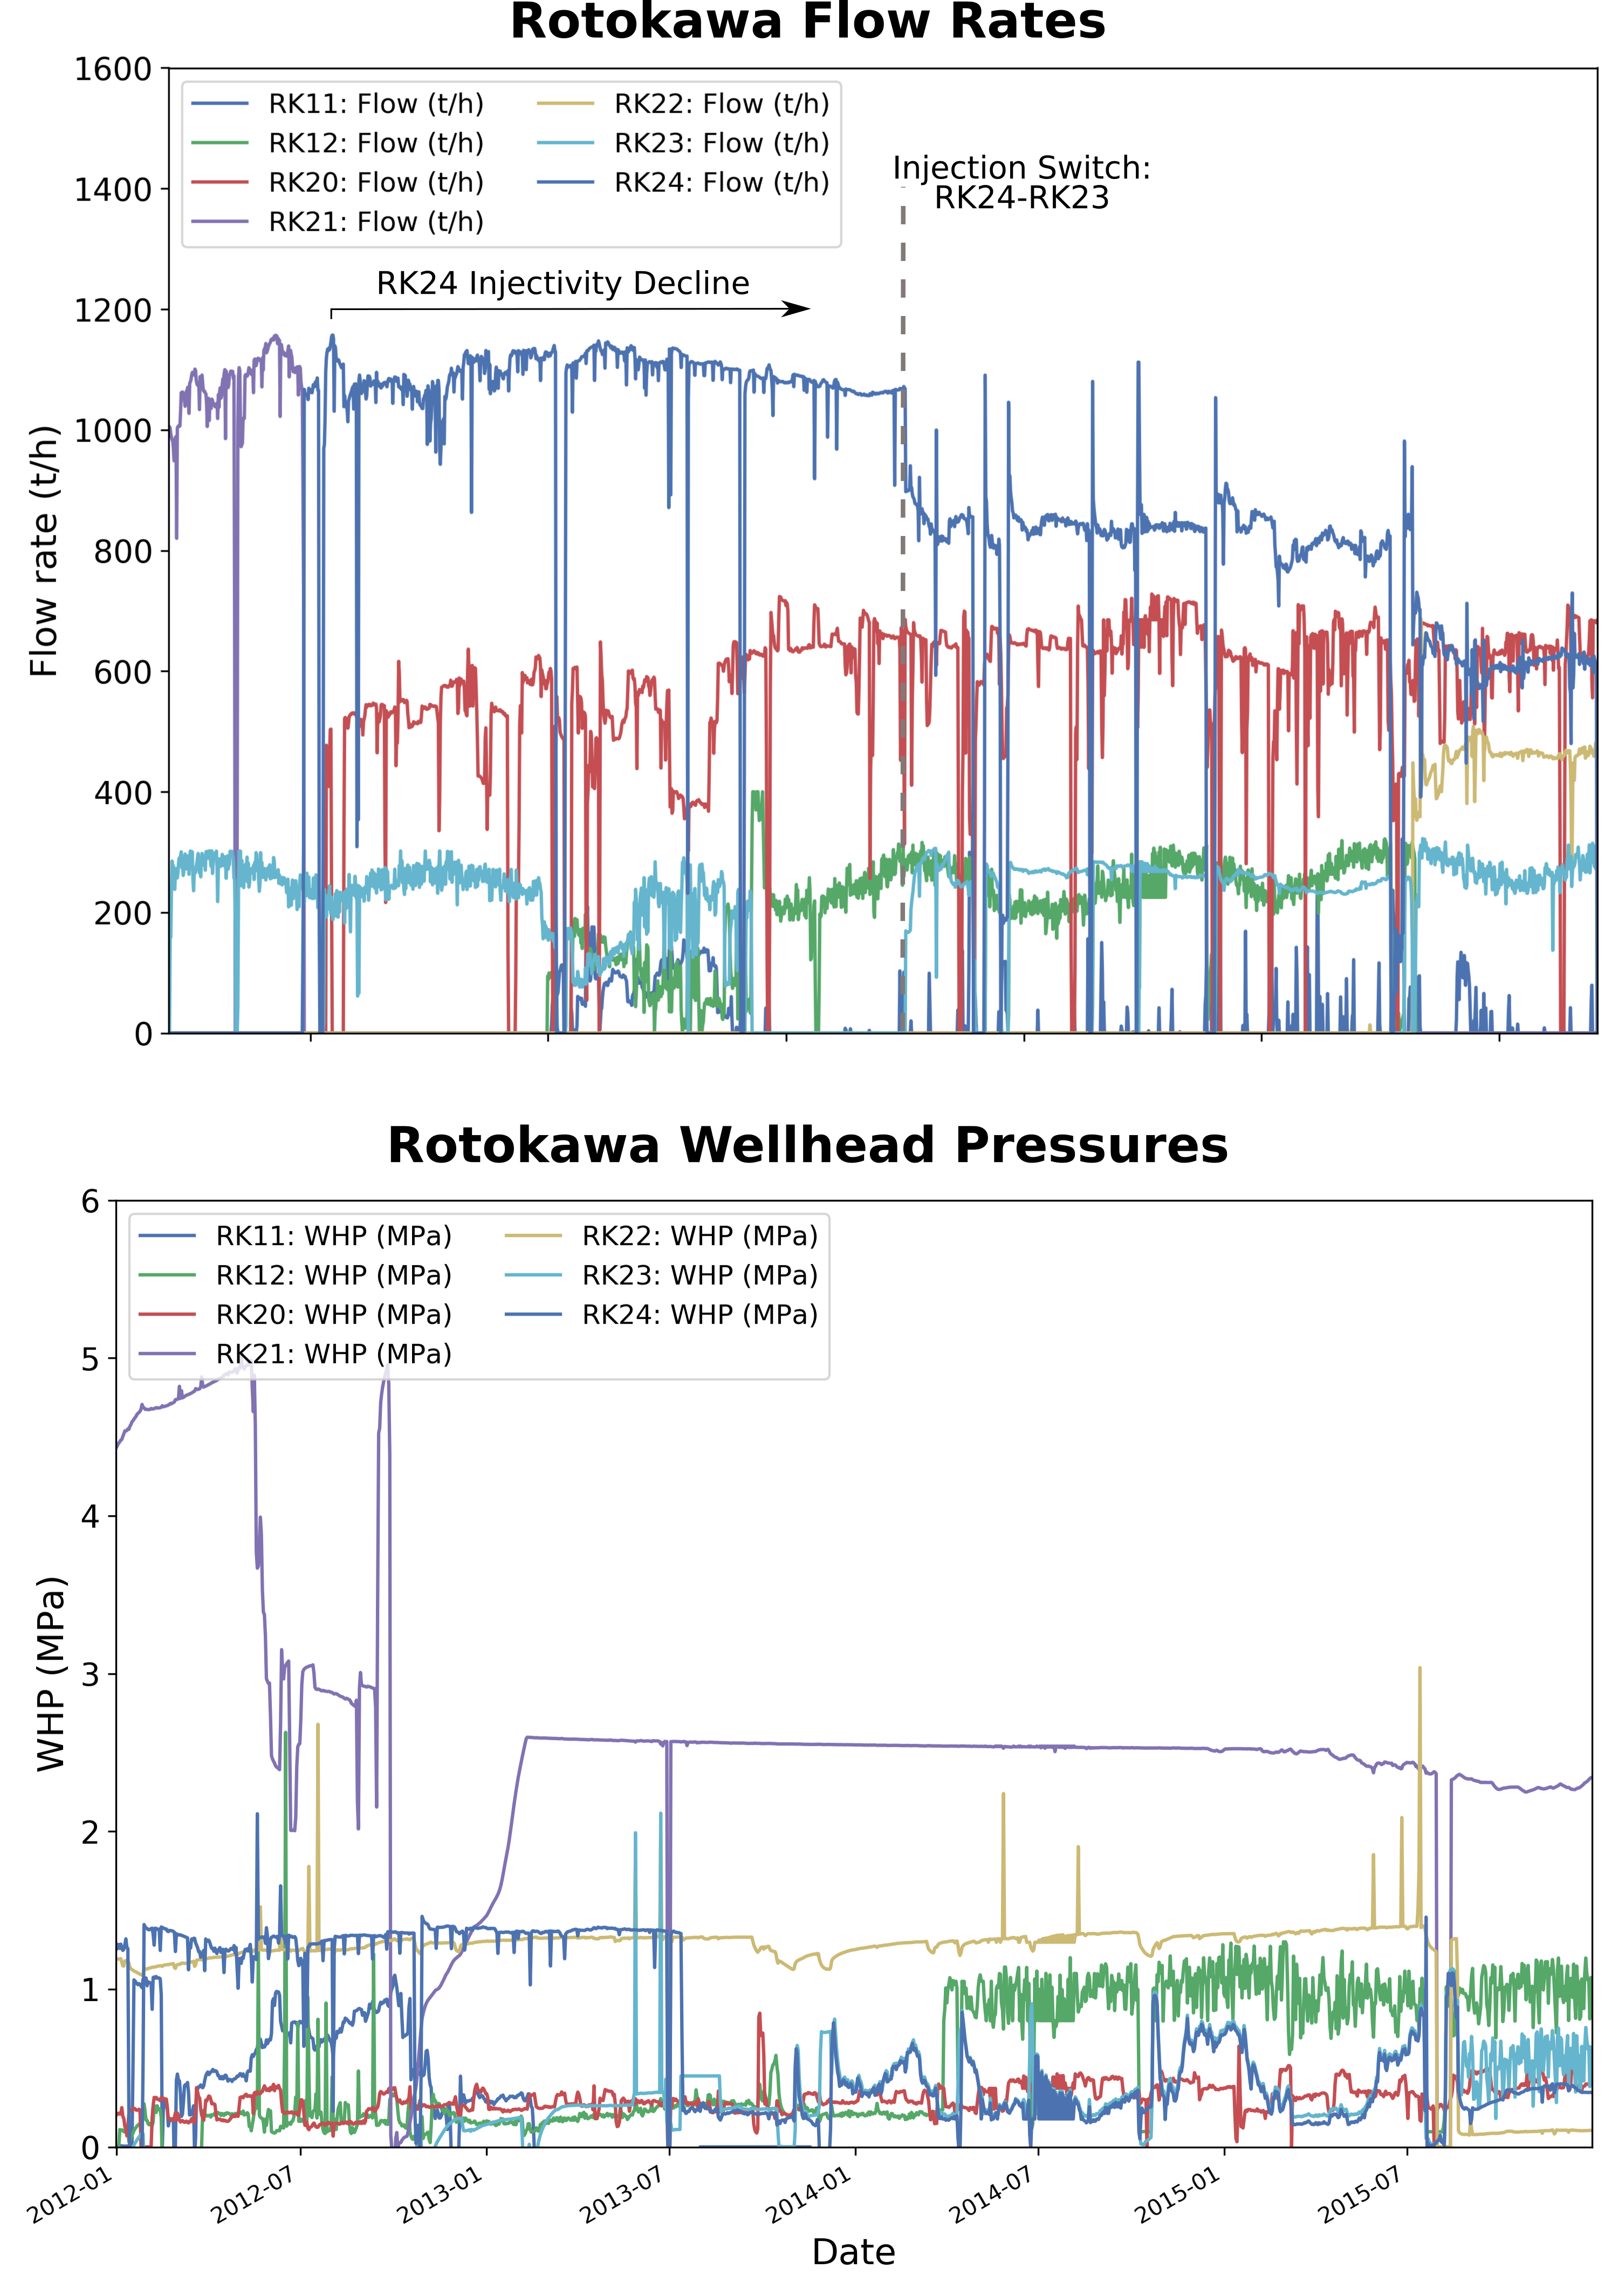
\includegraphics[width=0.84\columnwidth]{Chapter_1_Intro/figures/Rotokawa_overview_Intro/Rotokawa_overview_Intro_original}
\caption{{Overview of flow rates (top panel) and wellhead pressures (bottom panel)
from 2012 through 2015 for deep injection wells at Rotokawa. Selected
periods of interest as identified by Mercury are annotated on the flow
rate panel. RK34 was drilled from September to November 2014, but is not noted here due to a lack of flow data.
{\label{701773}}%
}}
\end{center}
\end{figure}\selectlanguage{english}

\begin{sidewaysfigure}[p]
\begin{center}
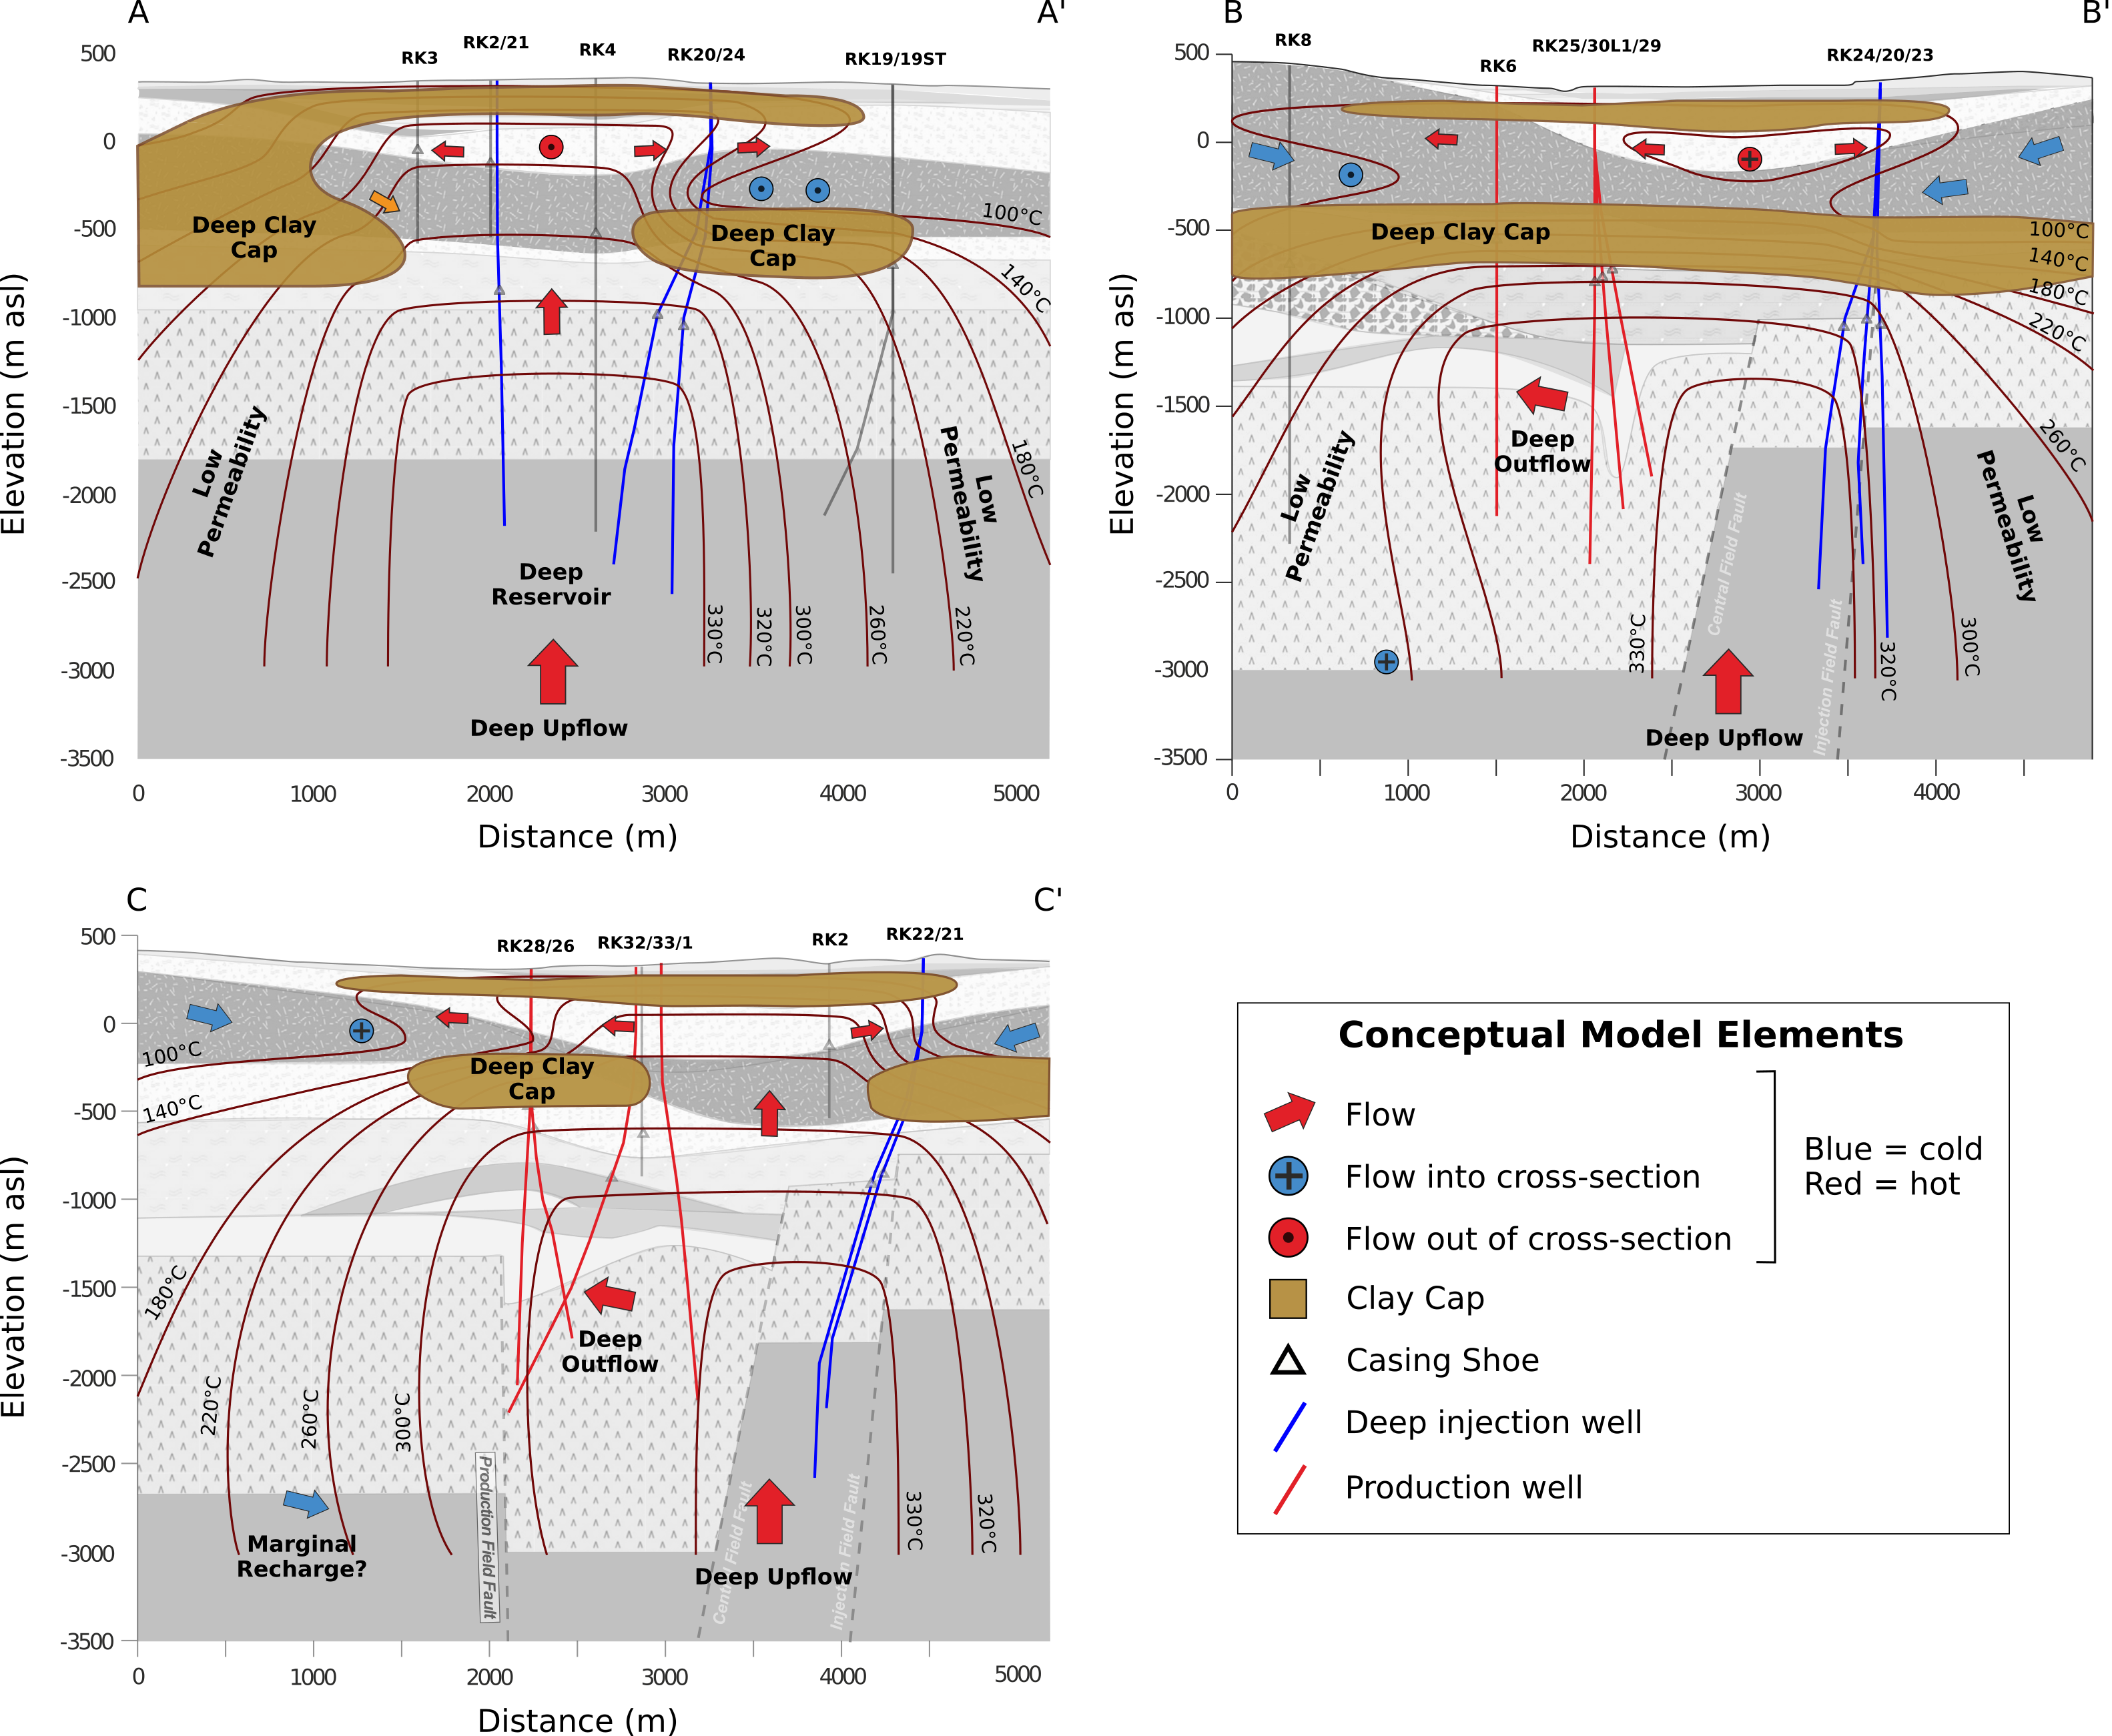
\includegraphics[width=0.7\textwidth,height=0.7\textheight,keepaspectratio]{Chapter_1_Intro/figures/Rotokawa_conceptual_11-22/Rotokawa_conceptual_2-20}
\caption{{Elements of the current Rotokawa conceptual model
from~\protect\citet{Sewell_2015} overlain on the geologic cross sections shown in
Figure~{\ref{599670}}. Maroon lines are isotherms
modeled from well temperature profiles. Arrows show the directions and
temperature of flow in the current reservoir conceptual model
(blue=cold, red=hot).
{\label{889233}}%
}}
\end{center}
\end{sidewaysfigure}

\subsubsection{Conceptual Model}
The understanding of the Rotokawa reservoir has benefited from over 20 years of detailed study and characterization spanning two phases of development. As a result, the understanding of the reservoir and the nature of fluid flow within it is well developed \citep{Sewell_2015,Addison_2017stanford,wallis2013}. The hottest temperatures in the field are found in the southern injection zone, with a maximum temperature of 338\textdegree C measured in well RK22 (Figure \ref{838185}), but there are strong lateral gradients in the natural-state temperatures to the northeast and northwest \citep{Sewell_2015,wallis2013} (Figure \ref{889233}). The main upflow of \textgreater330\textdegree C fluid is located near wells RK21\slash{RK22}, although the southwest boundary of the reservoir and upflow has not been verified by drilling \citep{Sewell_2015,winick2011natural}. Similar to Ngatamariki, Rotokawa is overlain by separate intermediate and shallow aquifers, although the hydraulic connection between the deep reservoir and intermediate aquifer is more pronounced than the `leak' at Ngatamariki \citep{winick2011natural} (Figure \ref{889233}).

At Ngatamariki, the path of fluid flowing from injection to production is oriented N-S, oblique to the regional NE-SW structure. At Rotokawa, the injection-production flow path is oriented NW-SE, perpendicular to the structural trend. This geometry has implications for fluid flow through the reservoir, as faults (in this case) act as along-strike flow pathways and cross-strike flow barriers \citep{Addison_2017stanford,McNamara_2015,Sewell_2015}. The effects of these structural barriers can be seen across the field. The Central Field Fault effectively isolates the injection and production zones, allowing only $\sim$12\% of the tracer injected in the injection wells to return to the production field within 60 days \citep{Sewell_2015,addison2015rotokawa}. Similar tracer tests have shown the Production Field Fault to be a conduit for rapid along-strike returns within the production field, which prompted the shift of deep injection from the southwest production field to the current injection zone \citep{Sewell_2015,Addison_2017stanford}. The \acrfull{CFF} is also inferred to be the structure that controls the connection between the deep and intermediate aquifers, and its surface trace appears to control the locations of a number of surface features at the field \citep{winick2011natural}.

Patterns in pressure drawdown in the production field are elongate along-strike, also suggesting that fluid flow is restricted across the structural grain \citep{hernandez2015rotokawa,Sewell_2015,Quinao_2013stanford}. The magnitude of these pressure differentials suggests a high degree of compartmentalization in the reservoir (Figure \ref{838185}). For instance, the pressure drawdown at RK29 since commissioning of NAP was $\sim$0.4 \acrshort{MPa} as of 2015. However, at RK25\slash{RK30}, which are only $\sim$200 m from RK29 and drilled from the same wellpad, the pressure drawdown is roughly an order of magnitude greater, despite the fact that RK29 is the most productive well in the field \citep{Sewell_2015}. Similar NW-SE pressure differentials exist in the southwestern production field and the variations in pressure responses across the entire production field suggest at least three separate compartments \citep{hernandez2015rotokawa}. The currently accepted boundaries of the three production field compartments, as well as the injection field, which comprises a separate compartment, are shown in Figure \ref{838185}.

\subsubsection{Seismicity}
Workers at GNS Science and Mercury (Mighty River Power) examine the seismicity at Rotokawa on a yearly basis in an effort to monitor changes in the reservoir. However, the last detailed characterization was only conducted through 2012 \citep{Sewell_2015WGC,Sherburn_2015}. As expected, seismicity migrated in conjunction with evolving injection strategy. At the end of 2012, with injection occurring predominantly into the southeastern compartment of the reservoir, \citet{Sewell_2015WGC,Sherburn_2015} observed that seismicity occurred inside the white dotted diamond shown in Figure \ref{838185}, migrating from the southern half of the diamond in 2008 to the northern half by 2012. The location of the northwest segment of this diamond has also been used to infer the location of the \acrshort{CFF}. In addition, \citet{Sewell_2015WGC,Sherburn_2015} concluded that most seismicity at Rotokawa was induced mostly by stress changes associated with reservoir cooling and contraction, instead of by pore-pressure increase, due to the relatively small pressure buildup measured at the wells (no greater than 1.5 \acrshort{MPa}). In the analysis that follows, specifically in Chapters 4 and 5, we look to update this understanding of Rotokawa seismicity.

\section{Induced Seismicity}\label{IS}
The revelation that human activities can induce earthquakes occurred decades ago, but has received a large amount of attention recently due to a remarkable increase in the number of events in the central US and elsewhere \citep{Ellsworth_2013,Kim_2013,Keranen_2013,Kim_2013,Keranen_2013,Zoback_2012co2,Baisch_2006,Evans_2004,Deichmann_2009}. Human-triggered seismicity has in fact been observed for nearly a century in relation to the impoundment of large water reservoirs \citep[e.g.][]{carder1945seismic,Gupta_2018} and early oil and gas operations \citep{Hough_2016}. Following a high-profile case of IS at the Rocky Mountain Arsenal near Denver, CO in 1962 \citep{Healy_1968}, a controlled experiment at the Rangely oil field in Colorado demonstrated a convincing connection between fluid injection and seismicity \citep{Raleigh_1976}. Also starting in the 1960's, new hydraulic fracturing (i.e. `fracking') techniques were being used to rehabilitate old oil and gas reservoirs, but these operations garnered little attention as the volumes injected were relatively small and the targeted formations were relatively permeable, leading to little notable seismicity. In the 1990's, however, the combination of massive hydraulic fracturing and advances in horizontal drilling made possible fracking in tight, shale reservoirs and opened large parts of the aseismic interior US to large-volume fluid injection. The rapid deployment of these techniques in places such as Oklahoma, Ohio and Texas brought about noticeable increases in felt seismic events in these areas \citep{Ellsworth_2013} that have since been attributed to the injection of fracking wastewater and to fracking itself \citep[e.g.][]{Kim_2013,Keranen_2013,Kim_2013,Keranen_2013}.  These events heightened national attention for the topic of IS and spurred a continuing effort to understand what factors determine where and when injection operations will induce seismicity \citep[e.g.][]{Goebel_2018}.

\subsection{Settings of Injection IS}
Human-induced seismicity is related to a number of processes including mining or gas-related mass extraction and weapons testing \citep[e.g.][]{Chambers_2015,Kim_2007}. Here we focus on IS related to the injection of fluids into the subsurface, which generally occurs in three settings:
\begin{itemize}
  \item{\textbf{Oil and Gas Extraction}}
  
  As mentioned above, the bulk of the attention devoted to IS internationally is related to enhanced oil and gas recovery through massive hydraulic fracturing. Certain such cases have been directly attributed to the hydraulic fracturing treatments themselves \citep[e.g.][in Canada]{Atkinson_2016,Skoumal_2015}. However, the vast majority of cases, are induced by the deep disposal of fracking-related wastewater at or below the depths of the fracking wells \citep[e.g.][]{Kim_2013,Keranen_2013,Yeck_2017,McGarr_2017}. Many of these events are located at depths below that of the injection and occur on preexisting basement faults up to tens of km away from the injection well. The factors that determine whether seismicity will occur for a given scenario, and what the frequency and magnitude might be, are still a topic of active research.

  \item{\textbf{CO$_{2}$ Sequestration}}
  
  Over the past decade, the possibility of capturing CO$_2$ from industrial activities and reinjecting it into the subsurface has been raised as a potential strategy for mitigating human-induced climate change. As a result, a number of pilot projects exploring the efficacy of carbon capture and storage have been undertaken in various locations worldwide \citep{Evans_2012,Zoback_2012co2}. This process involves the injection of fluid (supercritical) CO$_2$ into the subsurface, and therefore may generate seismicity via the same processes involved with fracking-related seismicity \citep{2013}. Currently, the future risk of induced seismicity associated with these projects is difficult to determine. If this technology is to be adopted as a viable climate-change mitigation strategy, it will involve injected volumes many orders of magnitude larger than those related to the current pilot projects \citep{Zoback_2012co2}. However, even at these relatively small volumes, significant seismicity has been recorded in some locations \citep[e.g.][]{Goertz_Allmann_2017}.
  
  \item{\textbf{Geothermal Power Production}}
  
  As described above, power can be produced by `mining' heat from deep reservoirs in the earth's crust. These reservoirs can be divided into enhanced geothermal systems (EGS) and conventional reservoirs. In this thesis, we will deal with conventional reservoirs. However, the seismicity induced at EGS reservoirs is still relevant to the discussion of injection-induced seismicity, especially in medium to high-temperature reservoirs.
  
  The aim of EGS is to mine heat from hot, yet relatively impermeable, rock at drilling-accessible depths. Usually this is accomplished through injection of fluids at pressures sufficient to fracture the rock at depth (similar to oil and gas fracking) and/or shear preexisting faults and fractures in the reservoir (sometimes called `hydroshearing`), thereby creating a permeable reservoir between an injection and production well or wells. Enhanced geothermal systems were invented at a part of the Hot Dry Rock experiment in the 1970's by the Los Alamos National Laboratory \citep{2013} in New Mexico. Subsequent projects were undertaken in England, France, Germany and Japan, with varying degrees of success and in the last 15 years other projects have been undertaken in Australia, Sewden and Switzerland. In each of these cases, some amount of seismicity was induced \citep{2013,Baria_1989,Baisch_2006,Evans_2004,Deichmann_2009}.
  
  Conventional geothermal reservoirs are those which already have sufficient heat and permeability for a convective hydrothermal system to have developed \citep{Grant_2011}. In these cases, extraction of fluid for power production is relatively easy, as no permeability need be created. However, extraction of fluid can also deplete the resource and cause surface subsidence due to pressure drawdown \citep{Grant_2011}. Fluid is therefore injected into the reservoir as a means of pressure support and as a mitigation strategy to resource depletion. These types of reservoirs are mostly located in areas of active tectonics such as New Zealand, Iceland, Italy, the Phillipenes, Indonesia, California and Central America and have been associated with seismicity for decades \citep[e.g.][]{Batini_1985,Allis_1982}. Rotokawa and Ngatamariki are both high-temperature, fluid-dominated versions of the conventional geothermal reservoir and so are most directly comparable to these types of fields elsewhere.
\end{itemize}

\subsection{Mechanisms of IS}\label{mechanisms}
Slip occurs on a fracture or fault when the shear force acting upon it exceeds its frictional strength \citep{stein_2000}. This condition can be met through an increase in the shear stress or a decrease in the frictional strength. The conventionally accepted mechanism by which seismic slip is induced during fluid injection operations is the increase in pore fluid pressure (Figure \ref{469299}), which decreases the normal stress on the fracture, thereby reducing its frictional strength and allowing a rupture to nucleate \cite[e.g.][]{Majer_2007}. However, as has become more clear with the growing number of case studies, there are other process that play important roles in IS and interact in ways that are complex and poorly understood. The key mechanisms that induce seismicity during fluid injection include:
\begin{itemize}
  \item{\textbf{Pore-fluid Pressure Perturbation}}
  
  The simplest explanation for the occurrence of IS is pore-fluid pressure increase within a fracture network that is hydraulically connected to the injection well. In such a scenario, any pressure perturbation at the well diffuses through the fracture network at a rate that depends on hydraulic properties of the reservoir, specifically hydraulic diffusivity, $D$ (Section \ref{terms}). \citet{Shapiro_2002} developed a technique called seismicity-based reservoir characterization (SBRC) by which the hypocentral locations of induced events could be used to infer the hydraulic diffusivity of a reservoir. This technique is based on the assumption that IS is induced purely as a result of the pore-fluid pressure increase, originating at an injection well and diffusing outwards. This is sometimes refered to as the slow `Biot wave' \citep{Biot_1956}. The outward diffusion of fluid molecules defines an envelope of $r = \sqrt{4\pi{D}t}$ for homogenous, istropic media, within which elevated pore pressure decreases the effective normal stress acting on a fracture network. As a result, the entire network is brought closer to failure and seismicity is most likely to occur, especially on structures that were already critically-stressed. This technique has been shown to be effective at describing the spatio-temporal occurrence of seismicity for numerous injections \citep[e.g.][]{Shapiro_1997,Shapiro_2009,Parotidis_2004,Jeanne_2014} (Figure \ref{182804}). However, it must be noted that this approach ignores the possibility of triggering by poroelastic stress transfer or thermal stress changes.
\end{itemize}\selectlanguage{english}
\begin{figure}[h!]
\begin{center}
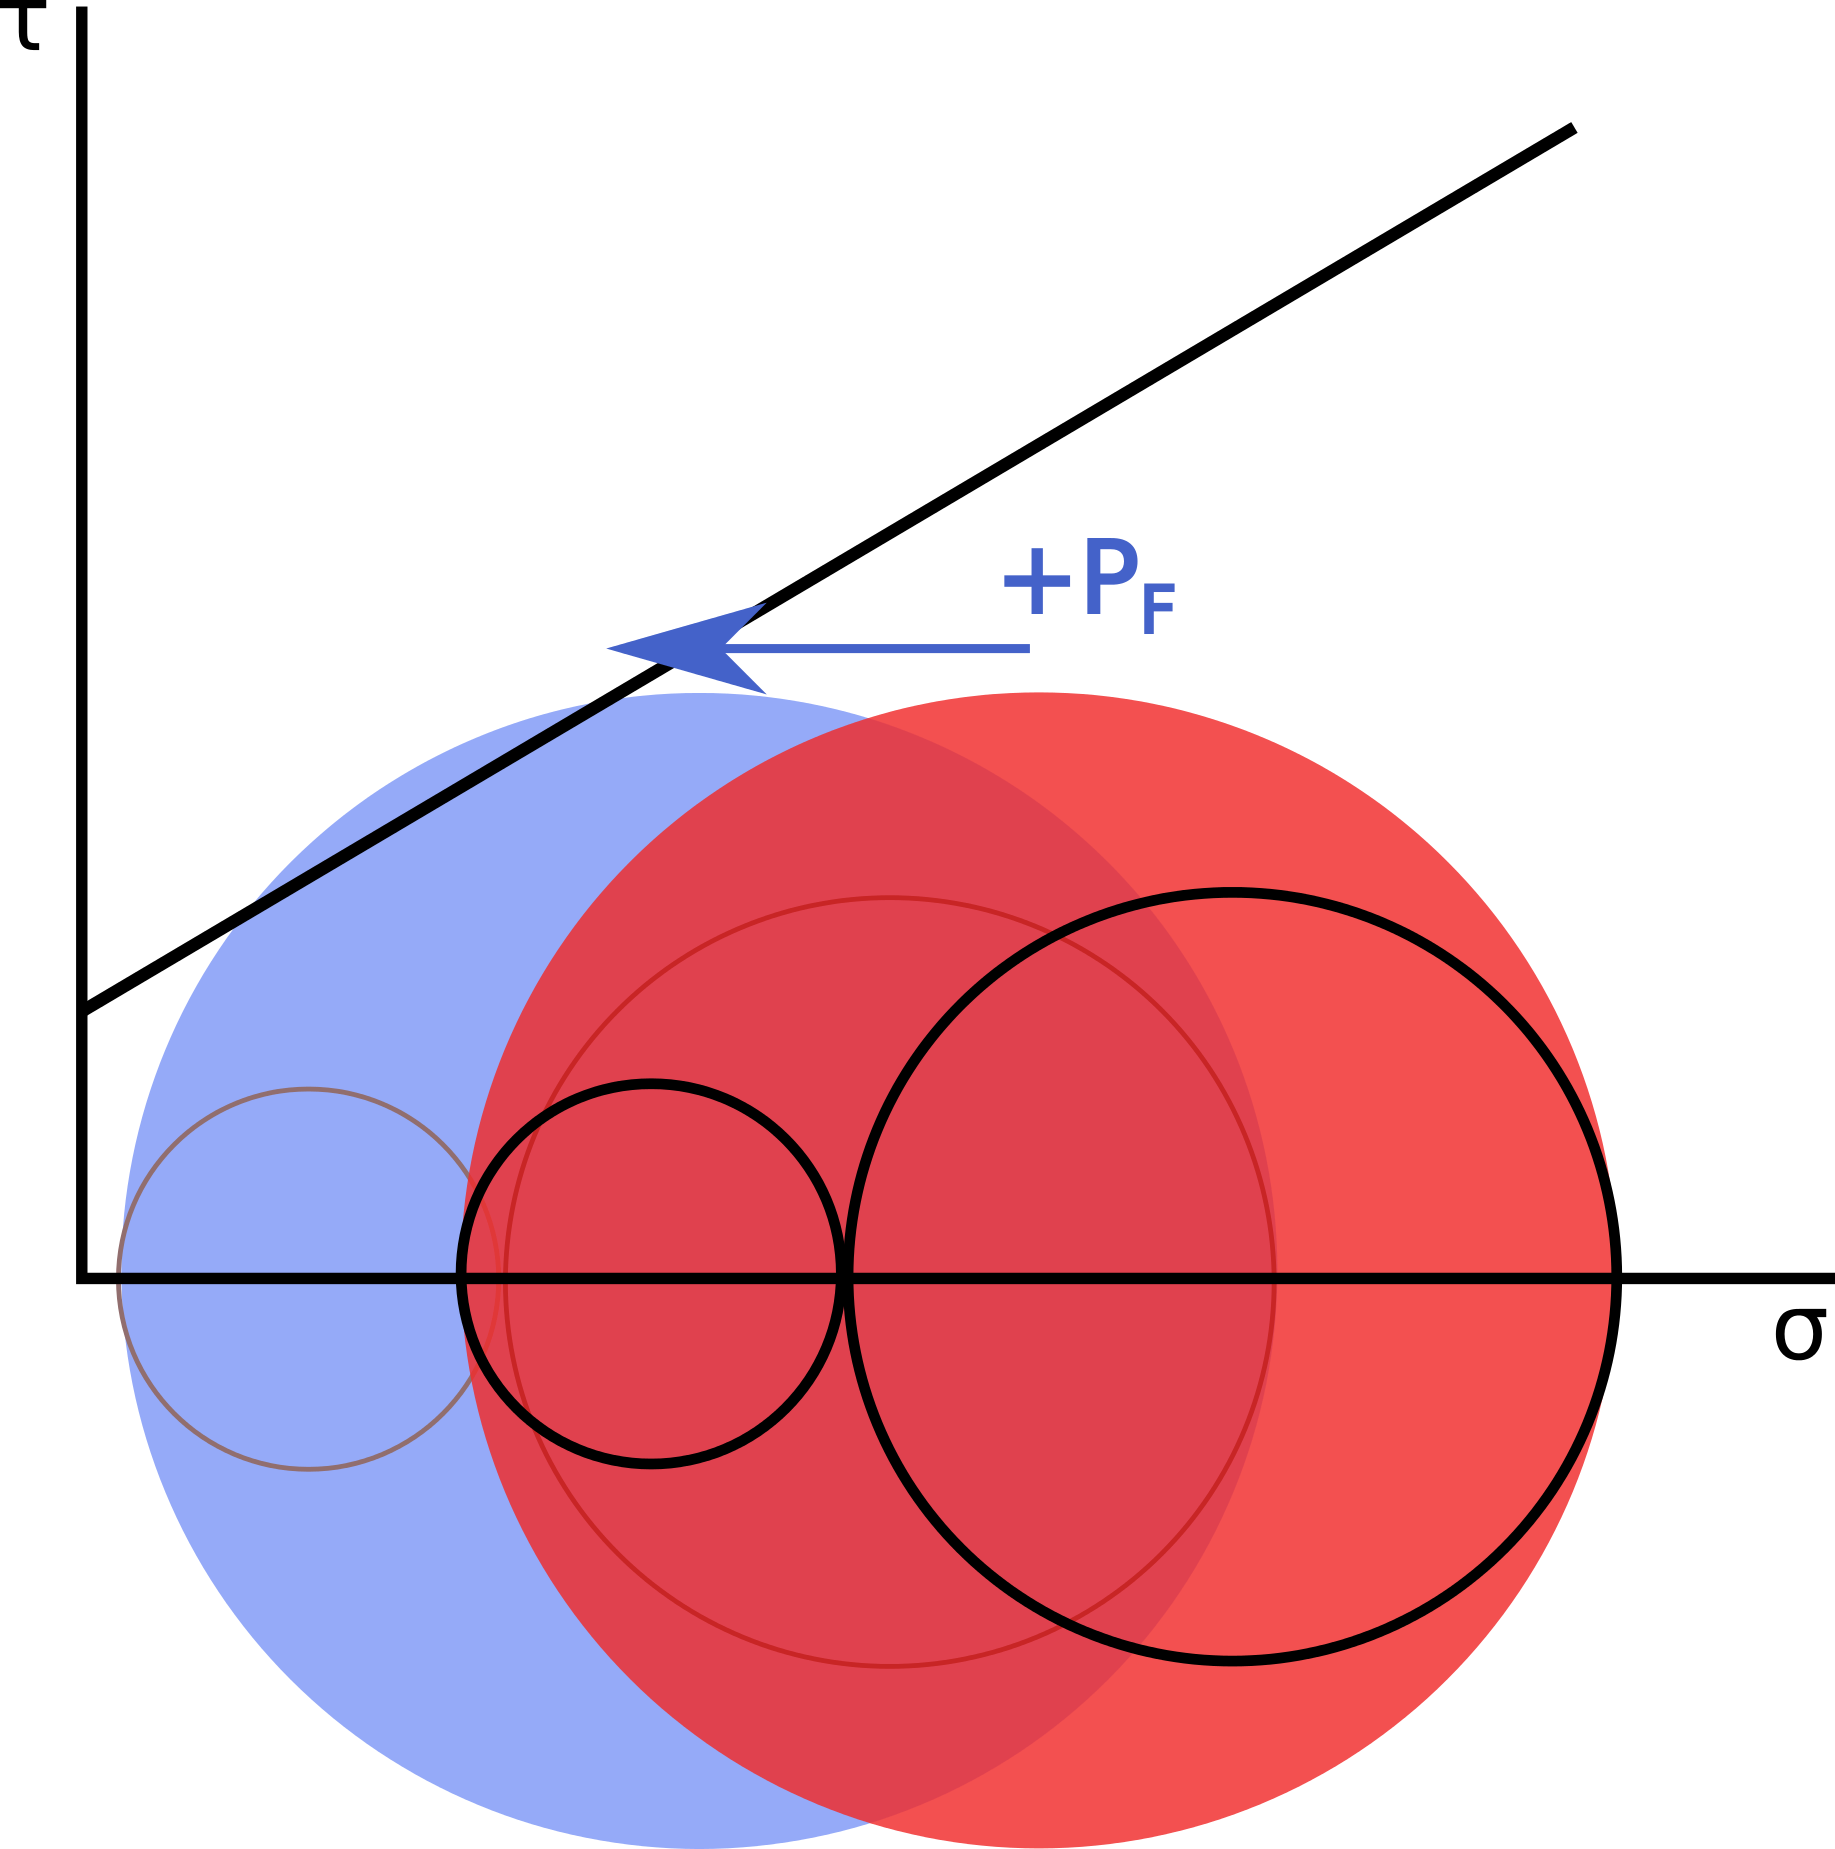
\includegraphics[width=0.42\columnwidth]{Chapter_1_Intro/figures/Pf_increase_mohr/Pf_increase_mohr_original}
\caption{{Schematic showing the shift in the hydrostatic Mohr circle (red) induced
by an increase in pore fluid pressure acting on a system of
fractures.~\(\tau\) signifies shear stress,~\(\sigma\)
normal stress and P\textsubscript{F} the pore-fluid pressure.
{\label{469299}}%
}}
\end{center}
\end{figure}\selectlanguage{english}
\begin{figure}[h!]
\begin{center}
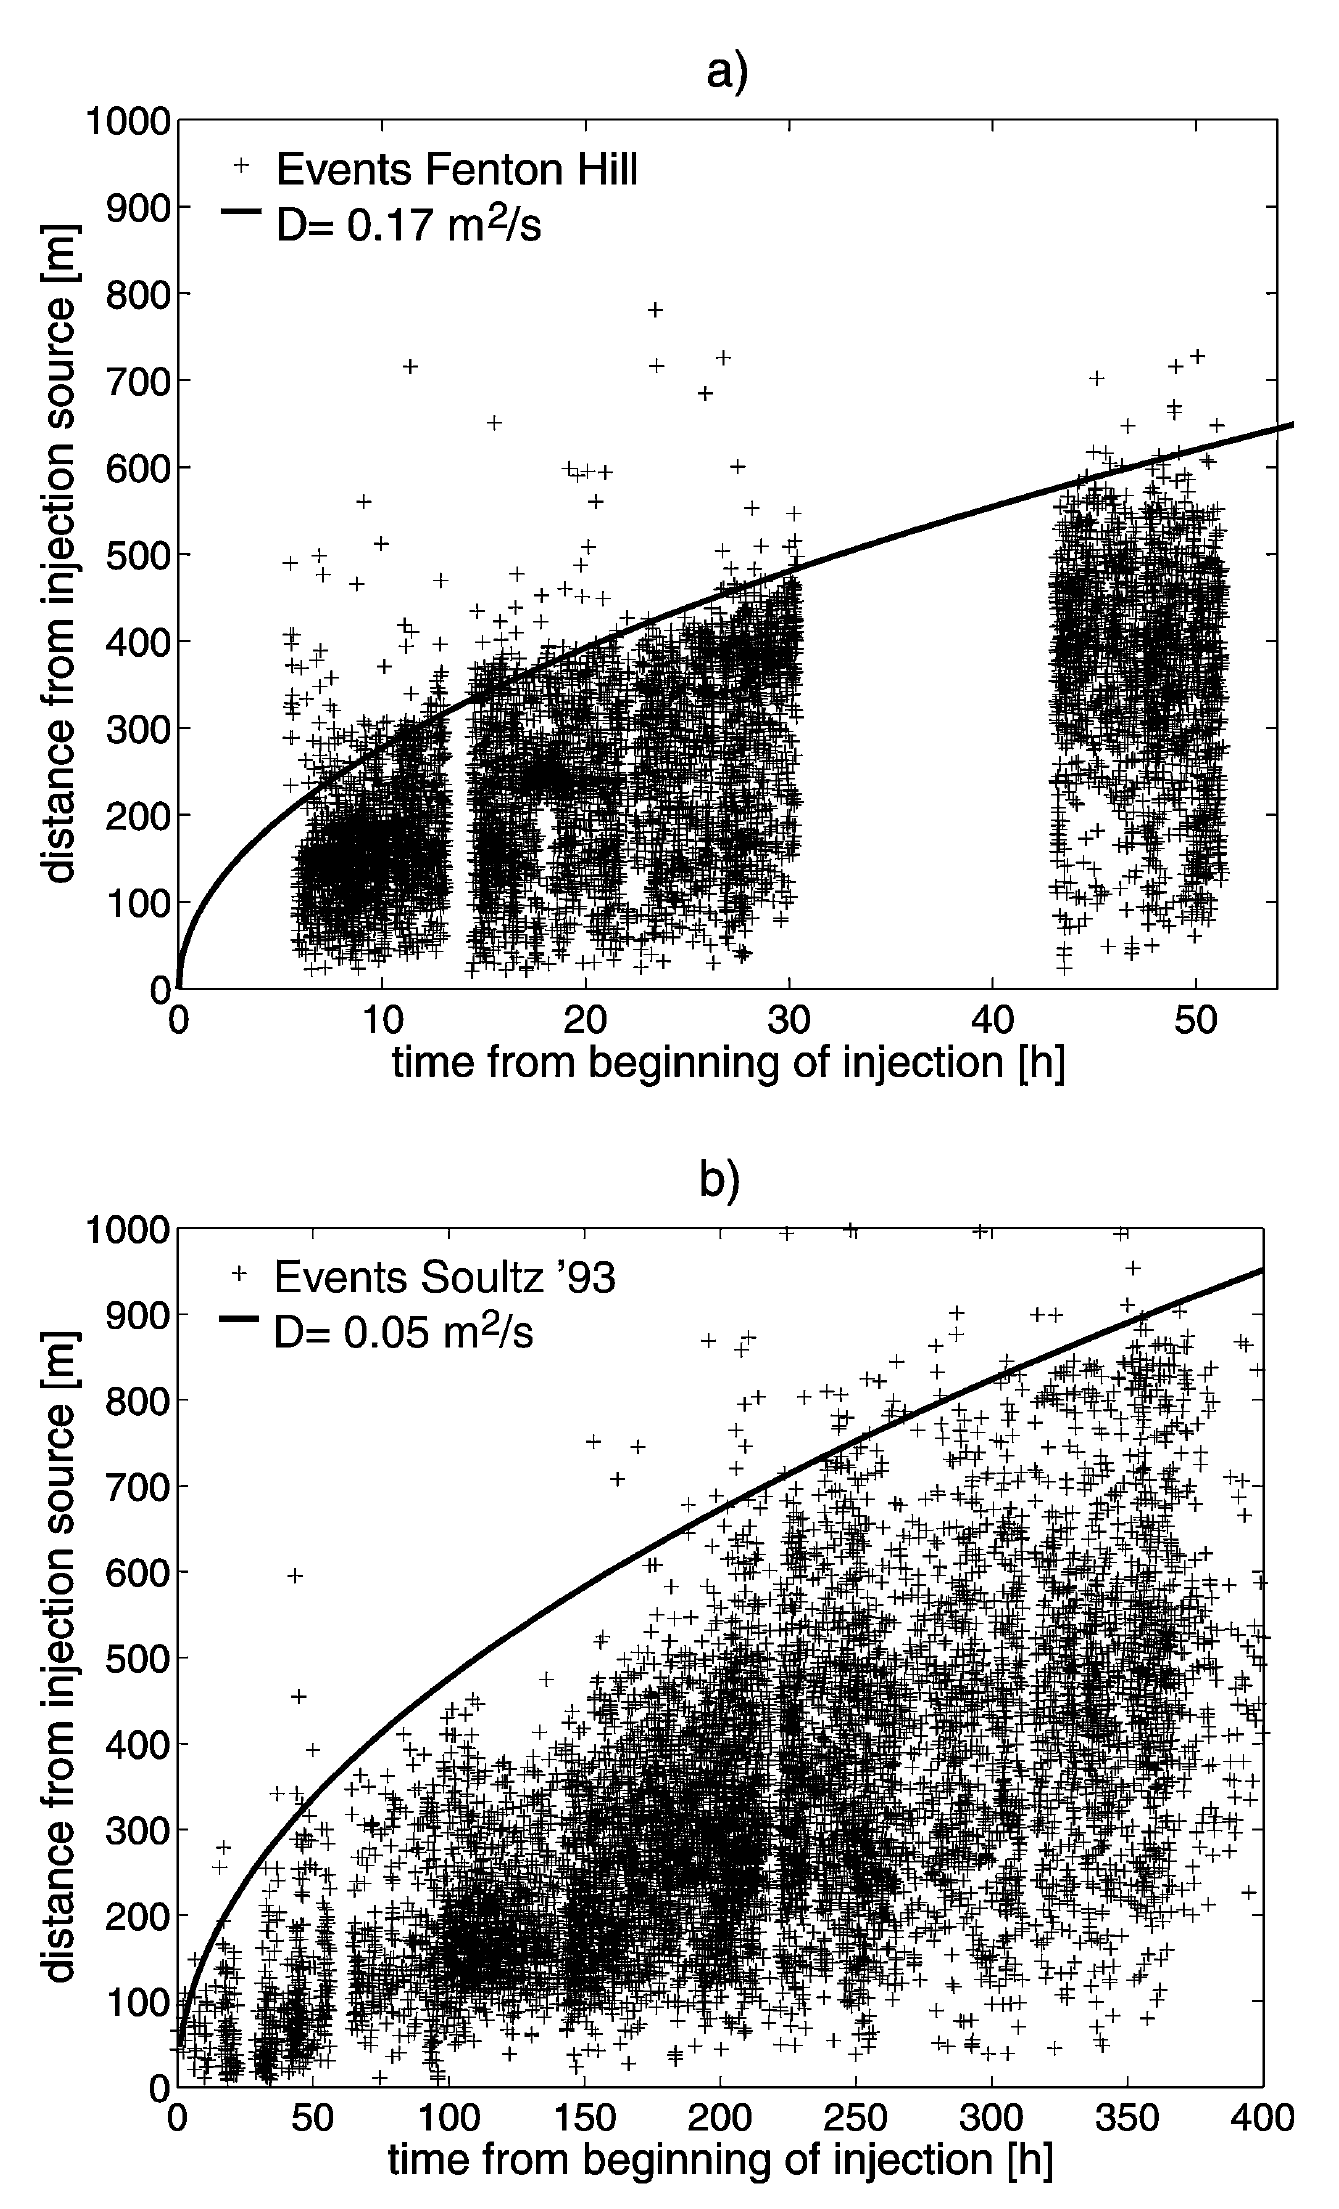
\includegraphics[width=0.70\columnwidth]{Chapter_1_Intro/figures/Shapiro_2002_SBRC_fig2/Shapiro_2002_SBRC_fig2_original}
\caption{{Typical `r-t' plots from~\protect\citet{Shapiro_2002} showing the triggering front
of seismicity as defined by SBRC for two injection operations: a) the
Fenton Hill, New Mexico Hot Dry Rock experiment and b) the Soultz EGS
project in France. Both sequences are well described by homogenous,
isotropic triggering fronts.
{\label{182804}}%
}}
\end{center}
\end{figure}

\begin{itemize}
  \item{\textbf{Poro-elastic Stress Transfer}}
  
  In addition to the perturbation of pore-fluid pressure, removal or injection of the large amounts of fluid from the subsurface induces related, and non-negligible, elastic stress changes due to the volume change of the reservoir \citep{2013}. In the case of depleted oil and gas reservoirs, or certain geothermal fields, this process can involve compaction of the reservoir and induce slip either within or outside the reservoir, depending on the prevailing tectonic regime \citep{Segall_1994,Segall_1998}. Where fluid is being injected into the reservoir, the corresponding increase in volume also induces a stress change. In the near-field (100s of m), the pore-fluid pressure increase experienced by fractures that are hydraulically connected to the injection well dominates the stress induced by volume change \citep{2013}. However, poroelastic stress transfer has been shown to dominate at greater distances and therefore, should not be ignored in assessing the effect of injection on IS \citep{Goebel_2017}. Recently, \citet{Goebel_2018} suggested that the degree to which either pore-pressure changes or poroelastic response dominate the seismic sequence is determined by the depth of injection with respect to basement. In their study, sub-basement injections were dominated by pore pressure increases and the associated seismicity terminated abruptly away from the well, whereas above basement injections were dominated by poro-elastic stress transfer and therefore had much wider spatial footprints and triggered larger magnitude events for a given injected volume \citep{Goebel_2018}. However, \citet{Hincks_2018} modeled the correlations between IS and a large number of operational and geological parameters for induced seismic sequences in Oklahoma and found a significant negative correlation between above-basement depths and seismic moment release. 
  
  An additional consideration for any seismic sequence, whether natural or induced, is the static (Coulomb) stress transfer associated with slip \citep{okada1992internal}. Coulomb stress change is known to explain the migration of aftershock sequences \citep[e.g.][]{Toda_2003}. It has also been shown to affect sequences of induced seismicity during EGS projects \citep{Catalli_2016,Schoenball_2012}. Though minor when compared to the other means of stress transfer considered in this section, it cannot be ignored.

  \item{\textbf{Thermo-elastic Stress Transfer}}
  
  Finally, particularly when considering IS in geothermal reservoirs, thermoelastic effects are of paramount importance. A number of researchers, working at the Geysers geothermal field in northern California, have shown that injection-related cooling of the reservoir can induce large changes in the stress state, which affect the style and location of induced faulting \citep{Mart_nez_Garz_n_2014,Mart_nez_Garz_n_2013,Mart_nez_Garz_n_2017,Jeanne_2014,Jeanne_2015tensor}. This effect is less pronounced, or negligible for injection scenarios where the temperature contrast between the reservoir and injected fluid is small, but in the case of high-temperature geothermal fields (including Rotokawa and Ngatamariki), the contrast can be 200--300\textdegree C \citep[e.g.][]{Mart_nez_Garz_n_2014,Jeanne_2015tensor}. Figure \ref{621452} illustrates the affect of thermoelastic stress reduction on the stress state in a reservoir from a Mohr-Coulomb perspective. The key point, as explained by \citet{Jeanne_2014,Jeanne_2015tensor}, is that the stress reduction is greatest parallel to the direction of the fluid flow, as this is the axis of maximum contraction of the reservoir. The effect this causes on the reservoir stress state depends on the relationship between the directions of the three principal stress components and the direction of flow. In the case of cold-water injection into a hot resource, the initial flow from the well will be gravity driven (due to the density of the cold fluid) and therefore will preferentially reduce $\sigma_{V}$. In the case of the Geysers, or most TVZ geothermal fields, $\sigma_{V} = \sigma_{1}$ and so cold water injection would have the effect of reducing $\sigma_{1}$, thereby reducing differential stress and stabilizing the reservoir fracture network (Figure \ref{621452}, green circle). \citet{Jeanne_2014} were able to show that this effect acted to suppress seismicity within $\sim$200 m of the wellbore during the EGS demonstration in the northwest Geysers in 2010. However, once the injected fluid begins to migrate laterally, the direction of which is dictated by the reservoir permeability distribution, the along-flow horizontal stress component is preferentially reduced. If this component happens to be $\sigma_{3}$, then the reservoir differential stress is increased and the fracture network brought closer to a critically stressed state (Figure \ref{621452}, blue circle).
\end{itemize}\selectlanguage{english}

\begin{figure}[h!]
\begin{center}
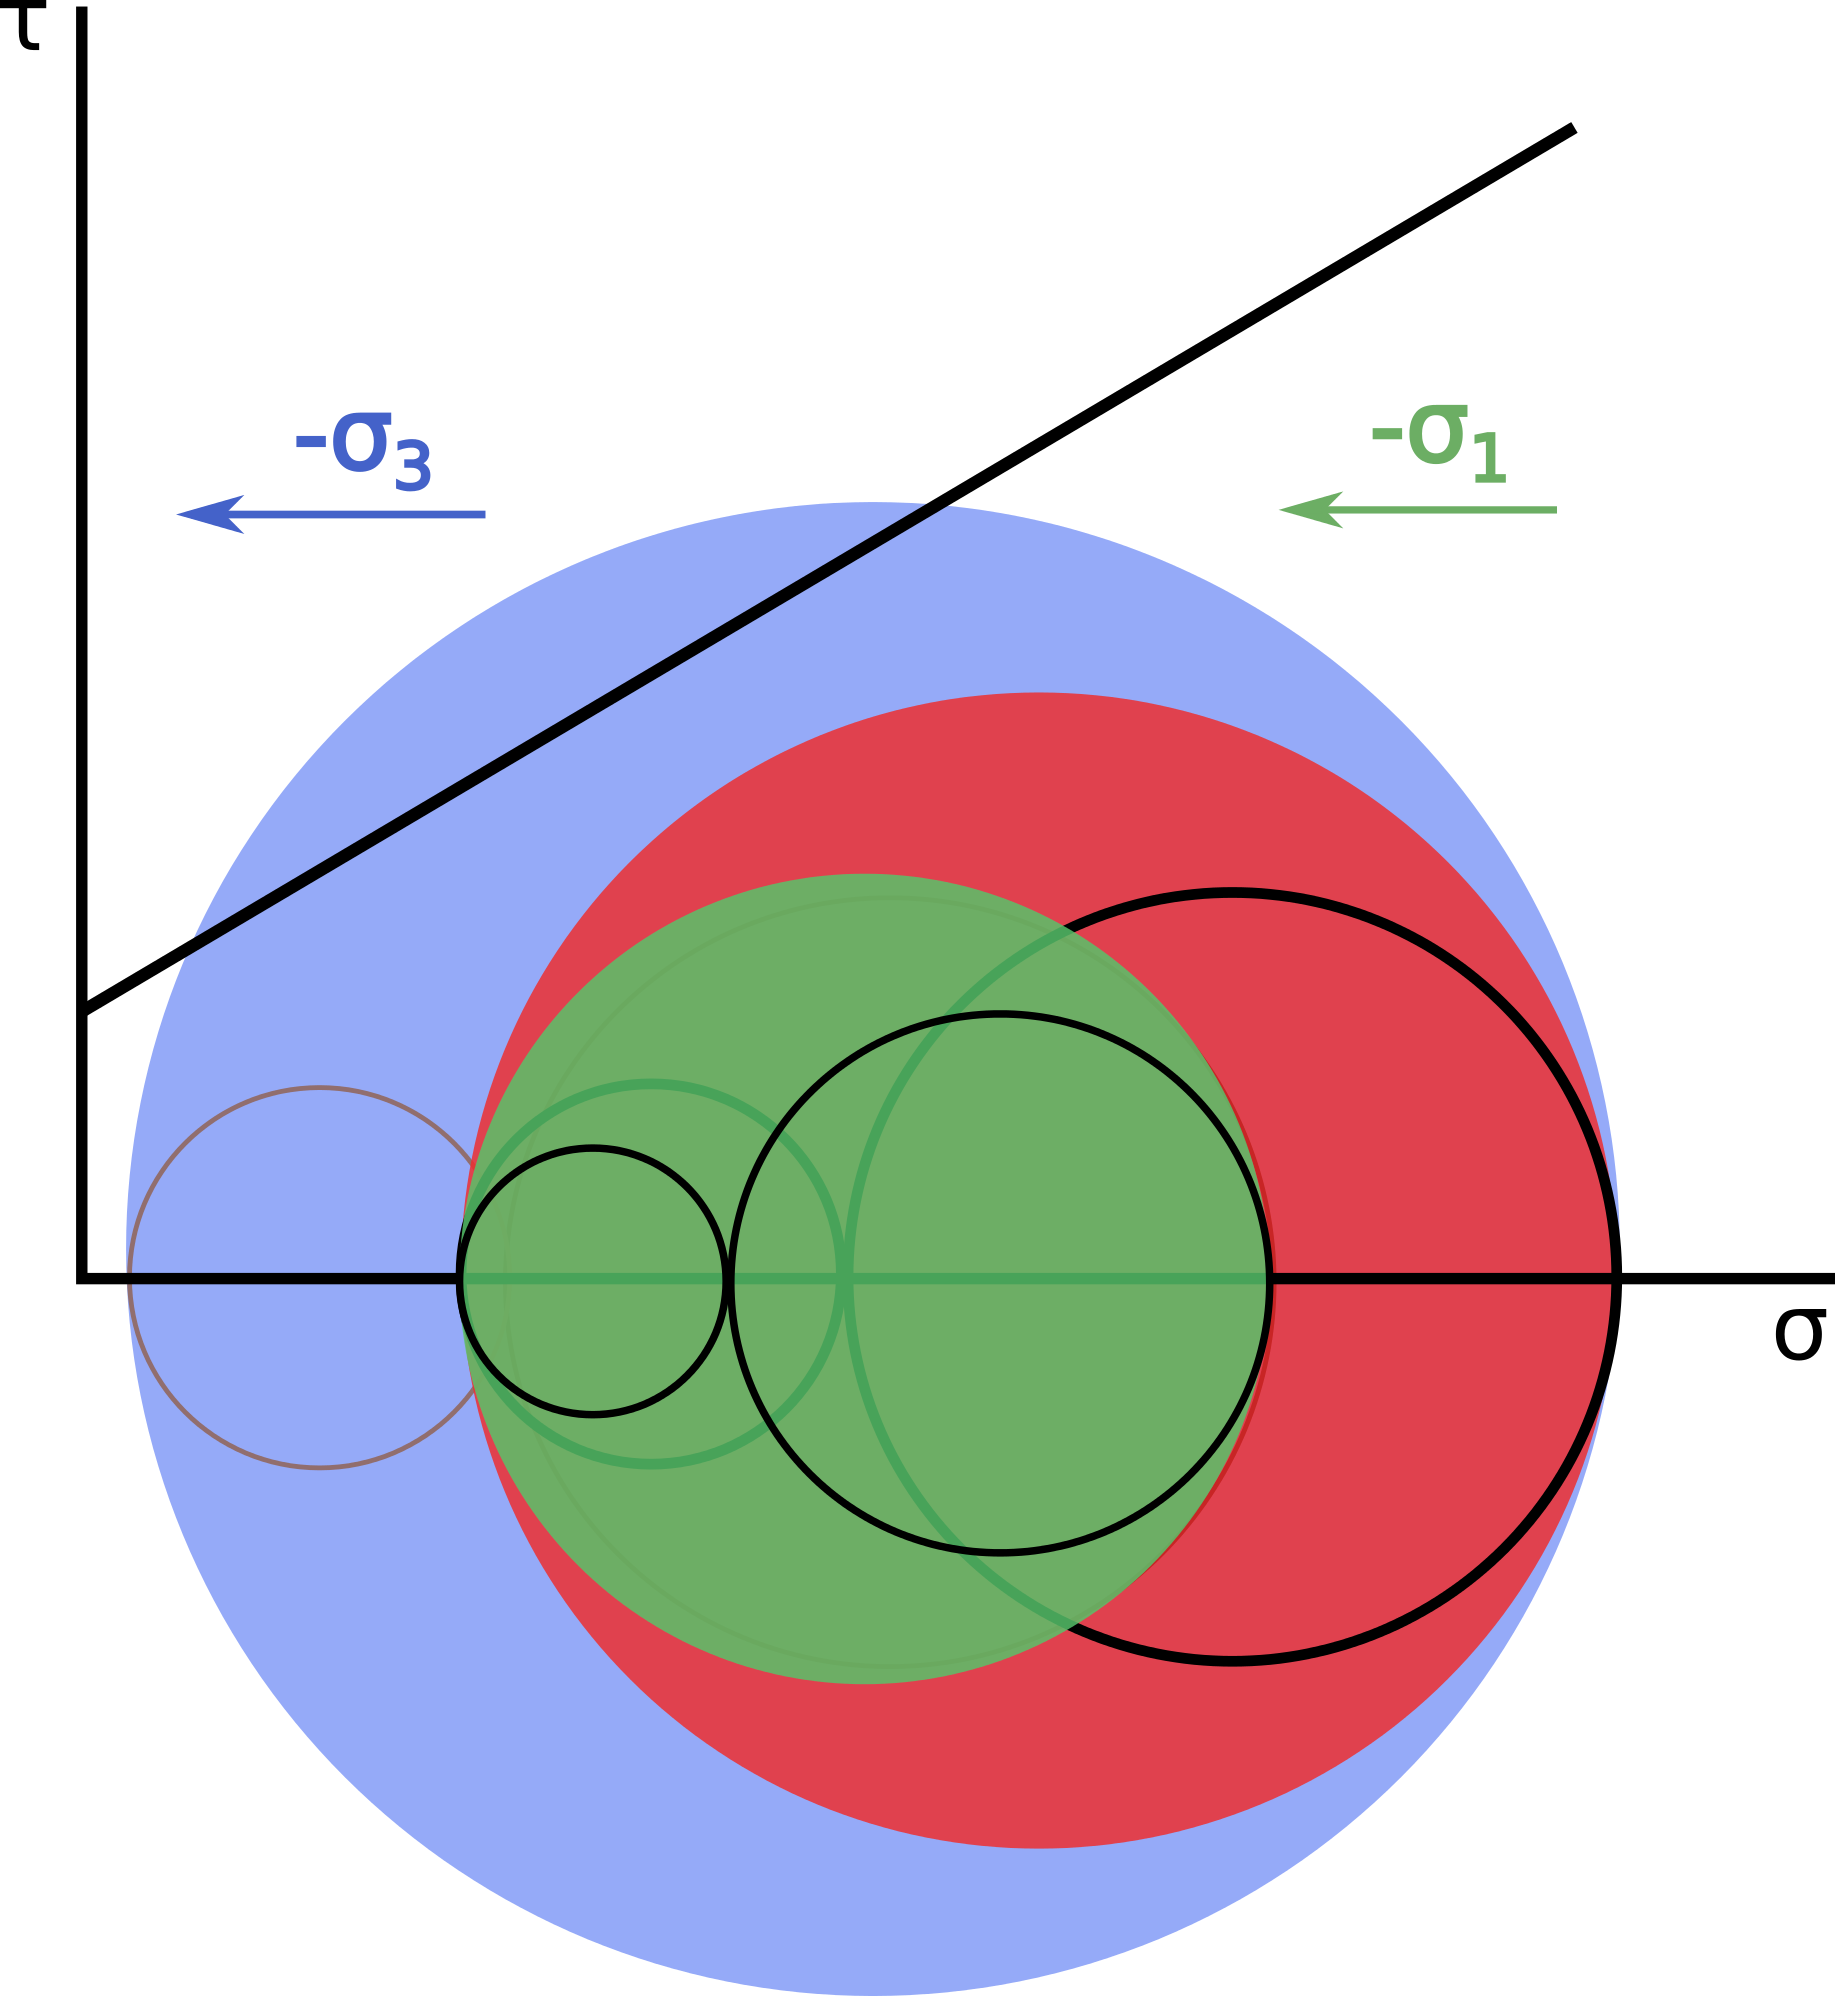
\includegraphics[width=0.42\columnwidth]{Chapter_1_Intro/figures/T_decrease_mohr/T_decrease_mohr_original}
\caption{{Schematic illustrating the changes in the Mohr circle induced by
thermoelastic stress changes in a reservoir due to the injection of cold
fluid, where the red circle represents the undisturbed state. The
induced change in the reservoir stress state is dependent upon the
direction of flow as it relates to the directions of the principal
stress axes. Cooling preferentially decreases the magnitude of stress
parallel to the direction of flow~\protect\citep{Jeanne_2014}. Therefore, the
blue circle illustrates the effect of fluid flow parallel
to~\(\sigma_{3}\), thereby increasing the differential stress and
bringing the fracture network closer to its critical stress state. If
fluid flow is parallel to~~~\(\sigma_{1} \), then differential stress
is decreased and the fracture network is made more stable. In the
normal-faulting stress state of the TVZ (\(\sigma_{1}\) is
vertical), the blue circle would correspond to a preferred NW-SE flow
direction, whereas NE-SW flow would reduce~\(\sigma_2\), a state
which would be represented by a Mohr circle equal in size to the red
circle, but with modified sizes of the subcircles. This would signify a
change in the orientation of fractures which would be able to fail.
{\label{621452}}%
}}
\end{center}
\end{figure}

\subsection{Permeability and Seismicity}
For most industrial applications of fluid injection, formation permeability is of paramount importance. Generally, fluid injection operations either seek to increase permeability (e.g. geothermal well stimulation, hydraulic fracturing) or require that sufficient permeability exists so that the formation will accept the fluid being injected (e.g. wastewater disposal, CO$_2$ sequestration, enhanced oil recovery) \citep{2013}. Induced seismicity, as it relates to any given injection, can be viewed in two lights: as a risk to be mitigated, or as a tool for tracking changes in the reservoir. When viewing IS as a potential risk, it must be weighed against the goals of the project, which often include increasing the formation permeability (e.g. fracking or geothermal stimulation). In these cases, operators must ask how much permeability gain is enough, and what level of seismicity is too much. At the same time, if IS is to be used as a monitoring tool (for instance, to map the stimulated volume of rock during an EGS project), operators need to know what information it provides. If the occurrence of seismicity implies a perturbation of pore-fluid pressure or reservoir stress change, does it also imply change in permeability? In order to satisfactorily answer these questions, the relationship between seismicity and reservoir permeability must be better understood.

The seismicity-permeability relationship has been widely studied in laboratory settings for a number of years \citep[e.g.][and citations therein]{Lee_2002}. Generally, when slip occurs on a preexisting fracture, the permeability of that fracture also increases through a process known as self-propping, where the misalignment of asperities on opposing fracture walls leads to an increase in fracture aperture, and thus permeability (Figure \ref{363218}). The degree to which fracture permeability is affected by slip depends on the length of the slip vector, rupture velocity, the roughness of the fracture surface and the material within the fracture (gouge) \citep{Fang_2017}. Fracture permeability can also increase as a result of displacement normal to the fracture plane through processes such as thermal contraction of the fracture walls or pore pressure increase (Figure \ref{363218}).

\citet{Guglielmi_2015} measured shear and normal displacement during injection into a decameter-scale fault and found that fault permeability was most sensitive to normal displacements early in the injection, with relatively little permeability gain related to shear displacements induced at later stages of the injection. This result questioned the commonly-held belief that the stimulation (i.e. permeability increase) of injection wells at sub-$\sigma_{3}$ pressures, was due to induced shear on hydraulically-connected fractures. Instead, the permeability increase could be largely due to normal displacements which were possibly aseismic. In turn, this called into question the use of seismicity as a way to map the extent of the stimulated reservoir \citep[e.g.][]{Fang_2018,Yoon_2014,Dempsey_2015}. This permeability-seismicity decoupling was recently illustrated through modeling of the Habanero and Paralana EGS project in Australia \citep{Riffault_2018}.

Aseismic motions are important contributors to permeability change in isothermal environments, such as shallow mines \citep{Guglielmi_2015}, or shale reservoirs \citep{Das_2011}. However, they may play an even more important role in high-temperature geothermal environments where thermoelastic contraction of fracture walls may serve to encourage fracture normal displacement. A model where well permeable zones expand and contract in response to thermal stresses is widely accepted at geothermal fields in New Zealand, where it has been used to describe oscillating injectivity behavior in response to injection-related cooling, and subsequent heating in the absence of injection \citep{grant2013thermal}.

A final, and more difficult to characterize, factor influencing reservoir permeability is fluid chemistry. As fluid moves through a formation, it may dissolve minerals out of, or precipitate minerals into, fractures, depending on the pressure and temperature and composition of the fluid. Though less well understood, this effect probably plays a large part in creating or destroying permeability through opening or sealing of fractures that would be likely to fail \citep{Clearwater_2015}. In this work, we will not address this issue, but it must be noted as a significant source of uncertainty with respect to reservoir permeability.\selectlanguage{english}

\begin{figure}[h!]
\begin{center}
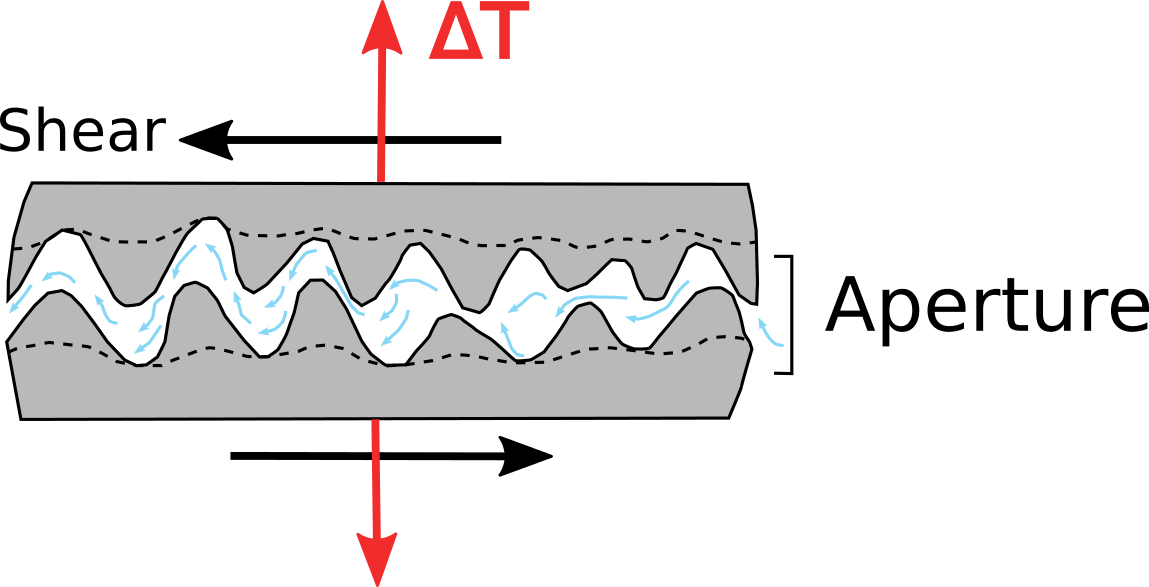
\includegraphics[width=0.70\columnwidth]{Chapter_1_Intro/figures/simple_stim_fig/simple_stim_fig_original}
\caption{{Simple schematic (adapted from \protect\citet{Fang_2017})~ illustrating the
possible fracture aperture increase associated with both slip on a fault
or fracture opening due to pressure increase, thermal contraction of the
fracture walls, or both.
{\label{363218}}%
}}
\end{center}
\end{figure}

\section{Thesis structure}
Chapter 2, following this introductory chapter, will discuss in detail the seismic data and network that provide the raw basis for all of this work. It will also touch on the supplemental data gathered by Mercury NZ, Ltd at the geothermal wells and will explain the basic methodologies used to detect and locate seismic events as well as the methods used to determine the magnitudes and focal mechanisms for well-recorded events.

Chapters 3, 4 and 5 contain distinct, standalone projects and have been written and formatted with the intent of publication.

Chapter 3 has been submitted to G-cubed as "Seismic Response to Injection Well Stimulation in a High-Temperature, High-Permeability Reservoir" and addresses the relationship between seismicity and injection during the stimulation and completion tests undertaken by Mercury prior to the startup phase of the Ngatamariki power plant.

Chapter 4 parallels Chapter 3, but at Rotokawa. It relates rates, locations and magnitudes of seismicity to changes in injection from 2012--2016. It also attempts to establish relationships between the frequency-magnitude distribution of Rotokawa seismicity and reservoir pressure distribution.

Chapter 5 details the spatial and temporal variations in source properties (i.e. focal mechanisms and magnitude) and stress at both Ngatamariki and Rotokawa between 2012 and 2015.

Finally, chapter 6 summarizes the findings of the preceding three chapters and suggests potential paths along which the research presented here could continue.

Chapters 3, 4 and 5 each contain detailed descriptions of the methodologies used. Therefore, chapter 2 will address only the methods used in creating the underlying earthquake catalog, which includes linear, grid-search and double difference earthquake locations, event magnitudes and event focal mechanisms. All further explanation of the more complex methods applied in the standalone chapters will therefore be addressed in the appropriate chapter.

The vast majority of the work presented in this thesis was conducted by me (Chet Hopp), however, I have chosen to write this thesis in the first-person plural, as is consistent with, and in acknowledgment of, the significant contributions of both my supervisors and colleagues, who have been included in chapter 3 as authors of the submitted manuscript. To this point, the initial, amplitude-based detection and linear location of the earthquake catalog from which this work began was conducted by a team of researchers at GNS Science in Wairakei and elsewhere, under contract with Mercury NZ, Ltd. This contribution was intrumental in directing the rest of this research and, because of this, deserves mentioning here.